\subsection{Node-level}

\subsubsection{Server (computation, HW accelerators)}\label{subsubsection: Server (computation, HW accelerators)}

\definition{Server}s are like ordinary PCs, usually more powerful, but with a \textbf{form factor that allows them to fit into the shelves} (such as rack, blade enclosure format, or tower; the differences are explained later). They are usually built in a tray or blade enclosure format, \textbf{housing the motherboard}, the \textbf{chipset}, and \textbf{additional plug-in components}.

\highspace
The \textbf{motherboard} acts as the central hub, \textbf{connecting all the crucial components of the server and enabling them to communicate and work together}.

It provides sockets and plug-in slots to install CPUs, memory modules (DIMMs), local storage (such as Flash SSDs or HDDs), and network interface cards (NICs) to satisfy the range of resource requirements.

\highspace
The \textbf{chipsets} and \textbf{additional components} are grouped in the following way:
\begin{itemize}
    \item Number and type of CPUs:
    \begin{itemize}
        \item From 1 to 8 CPU socket.
        \item Intel Xeon Family, AMD EPYC, etc.
    \end{itemize}

    \item Available RAM:
    \begin{itemize}
        \item From 2 to 192 DIMM Slots.
    \end{itemize}

    \item Locally attached disks:
    \begin{itemize}
        \item From 1 to 24 Drive Bays. 
        \item HDD or SSD.
        \item SAS (higher performance but more expensive) or SATA (for entry-level servers).
    \end{itemize}

    \item Other special purpose devices:
    \begin{itemize}
        \item From 1 to 20 GPUs per node, or TPUs.
        \item NVIDIA Pascal, Volta, etc.
    \end{itemize}
    
    \item Form factor:
    \begin{itemize}
        \item From 1 unit to 10 units.
        \item Tower.
    \end{itemize}
\end{itemize}

\newpage

\begin{center}
    \textcolor{Red2}{\textbf{Differences between Rack, Blade and Tower}}
\end{center}

\subsubsection*{Tower Server}

A \definition{Tower Server} looks and feels much like a \textbf{traditional} tower \textbf{PC}.

\begin{flushleft}
    \textcolor{Green3}{\faIcon{check} \textbf{Advantages}}
\end{flushleft}
\begin{itemize}[label=\ding{51}]
    \item \textbf{Scalability} and \textbf{ease of upgrade}. Customized and upgraded based on necessity.

    \item \textbf{Cost-effective}. Tower servers are probably the \emph{cheapest of all kinds of servers}.

    \item \textbf{Cools easily}. Since a tower server has a low overall component density, it cools down easily.
\end{itemize}

\begin{flushleft}
    \textcolor{Red2}{\faIcon{thumbs-down} \textbf{Disadvantages}}
\end{flushleft}
\begin{itemize}[label=\ding{55}]
    \item \textbf{Consumes a lot of space}. These servers are difficult to manage physically.

    \item \textbf{Provides a basic level of performance}. A tower server is \emph{ideal for small business that have a limited number of clients}.

    \item \textbf{Complicated cable management}. Devices aren't easily routed together.
\end{itemize}

\newpage

\paragraph{Rack Servers}

\definition{Rack Servers} are unique \textbf{shelves that accommodate all the IT equipment} and allow their interconnection. The racks are used to store these rack servers.

\highspace
Server racks are measured in \definition{Rack Units}, or "U". One U is approximately 44.45 millimeters. The \underline{main advantage} of these racks is that they \textbf{allow designers to stack up other electronic devices and servers}.

\highspace
A rack server is designed to be positioned in a bay by vertically stacking servers one over the other along with other devices (storage units, cooling systems, network peripherals, and batteries).

\begin{flushleft}
    \textcolor{Green3}{\faIcon{check} \textbf{Advantages}}
\end{flushleft}
\begin{itemize}[label=\ding{51}]
    \item \textbf{Failure containment}. Very little effort to identify, remove, and replace a malfunctioning server with another.

    \item \textbf{Simplified cable management}. Easy and efficient to organize cables.

    \item \textbf{Cost-effective}. Computing power and efficiency at relatively lower costs.
\end{itemize}

\begin{flushleft}
    \textcolor{Red2}{\faIcon{thumbs-down} \textbf{Disadvantages}}
\end{flushleft}
\begin{itemize}[label=\ding{55}]
    \item \textbf{Power usage}. Needs of additional cooling systems due to their high overall component density, thus consuming more power.

    \item \textbf{Maintenance}. Since multiple devices are placed in racks together, maintaining them gets considerably though with the increasing number of racks.
\end{itemize}

\newpage

\paragraph{Blade Servers}

\definition{Blade Servers} are the latest and the most advanced type of servers in the market. They can be termed hybrid rack servers, where servers are placed inside blade enclosures, forming a blade system.

\highspace
The \textbf{most significant advantage} of blade servers is that these servers are the \textbf{most minor types of servers available now} and are \textbf{great for conserving space}.

\highspace
Finally, a blade system also meets the IEEE standard for rack units, and each rack is measured in the units of "U".

\begin{flushleft}
    \textcolor{Green3}{\faIcon{check} \textbf{Advantages}}
\end{flushleft}
\begin{itemize}[label=\ding{51}]
    \item \textbf{Size and form factor}. They are smallest and the most compact servers, requiring minimal physical space. Blade servers offer \emph{higher space efficiency} compared to traditional rack-mounted servers.

    \item \textbf{Cabling}. Blade server don't involve the cumbersome tasks of setting up cabling. Although you still might have to deal with the cabling, it is near to negligible when compared to tower and rack servers.

    \item \textbf{Centralized management}. Blade enclosures typically come with centralized management tools that allow administrators to easily monitor, configure and update all blades from a single interface.

    \item \textbf{Load balancing, failover, scalability}. Uniform system, shared components (including network), simple addition/removal of servers.
\end{itemize}

\begin{flushleft}
    \textcolor{Red2}{\faIcon{thumbs-down} \textbf{Disadvantages}}
\end{flushleft}
\begin{itemize}[label=\ding{55}]
    \item \textbf{Expensive configuration and Higher initial cost}. Although upgrading the blade server is easy to handle and manage, the initial configuration or the setup requires more effort and higher initial investment.

    \item \textbf{Vendor Lock-In}. Blade servers typically require the use of the manufacturer's specific blades and enclosures, leading to vendor lock-in. This can limit flexibility and potentially increase costs in the long run.

    \item \textbf{Cooling}. Blade servers come with high component density. Therefore, special accommodations have to be arranged for these servers to ensure they don't get overheated. Heating, ventilation, and air conditioning systems (HVAC) must be carefully managed and designed.
\end{itemize}

\newpage

\paragraph{Machine Learning}

\begin{deepeningbox}[: Machine Learning (supervised learning)]
    \textbf{Machine learning} (ML) is a branch of artificial intelligence (AI) and computer science that focuses on the using data and algorithms to enable AI to imitate the way that humans learn, gradually improving its accuracy (\href{https://www.ibm.com/topics/machine-learning}{source}).

    \highspace
    \href{https://ischoolonline.berkeley.edu/blog/what-is-machine-learning/}{UC Berkeley} breaks out the learning system of a machine learning algorithm into three main parts:
    \begin{enumerate}
        \item A Decision Process: In general, machine learning algorithms are used to make a prediction or classification. Based on some input data, which can be labeled or unlabeled, your algorithm will produce an estimate about a pattern in the data.

        \item An Error Function: An error function evaluates the prediction of the model. If there are known examples, an error function can make a comparison to assess the accuracy of the model.

        \item A Model Optimization Process: If the model can fit better to the data points in the training set, then weights are adjusted to reduce the discrepancy between the known example and the model estimate. The algorithm will repeat this iterative \dquotes{evaluate and optimize} process, updating weights autonomously until a threshold of accuracy has been met.
    \end{enumerate}

    \highspace
    The main goal is to learn a target function that can be used for prediction. Given a training set of labeled examples $\left\{\left(x_{1}, y_{1}\right), \dots, \left(x_{n}, y_{n}\right)\right\}$, estimate the prediction function $f$ by minimizing the prediction error on the training set:
    \begin{equation*}
        y = f\left(x\right)
    \end{equation*}
    Where $y$ is the output, $f$ is the prediction function and the $x$ is an image feature.
\end{deepeningbox}

\begin{deepeningbox}[: Artificial Neural Network]
    The \textbf{Artificial Neural Network} is a computational model inspired by the human brain (perceptron). It consists of interconnected nodes (neurons) organized in layers to process and analyze data and used to learn data representation from data (learn features and the classifier/regressor).

    \highspace
    The learning process of a Neural Network is as follows: Neurons make decisions (activation functions). There are wights, so the connections between neurons are strengthened or weakened through training- randomly initialized.

    The (training data) Neural Networks learn from historical data and examples. Then, labeled data are provided.
\end{deepeningbox}

\begin{deepeningbox}[: effects of ML and ANN]
    Deep learning models began to appear and be widely adopted, enabling specialized hardware to power a broad spectrum of machine learning solutions.
    
    Since 2013, AI learning compute requirements have doubled every 3.5 months (vs. 18-24 months expected from \href{https://en.wikipedia.org/wiki/Moore's_law}{Moore's Law}).

    To satisfy the growing compute needs for deep learning, \textbf{WSCs deploy specialized accelerator hardware}:
    \begin{itemize}
        \item Graphical Processing Units (GPUs) are used for data-parallel computations (the same program is executed on many data elements in parallel). In order to use parallel programming, high-level languages such as CUDA, OpenCL, OPENACC, OpenMP, and SYCL exist. This technique allows up to 1000x faster than CPU.


        \item Tensor Processing Unit (TPU), where Tensor is a n-dimensional matrix, are used for training and inference.


        \item Field-Programmable Gate Array (FPGA) are programmable hardware devices. The device user can program an array of logic gates (\dquotes{configured}) in the field instead of the people who designed it. An array of carefully designed and interconnected digital subcircuits that efficiently implement common functions, offering very high levels of flexibility. The digital subcircuits are called configurable logic blocks (CLBs).

        FPGA Applications in Data Centers:
        \begin{itemize}
            \item Network acceleration: FPGAs can offload specific processing tasks from CPUs, improving overall network performance and reducing CPU workload.

            \item Security acceleration: Encryption, decryption, and other security-related tasks can be accelerated using FPGAs, enhancing data centre security while maintaining performance.

            \item Data analytics: FPGAs can accelerate specific algorithms in data analytics workloads, leading to faster data processing and analysis.

            \item Machine learning: FPGAs can be configured to efficiently implement specific machine learning algorithms, potentially offering performance advantages for specialized tasks.
        \end{itemize}
    \end{itemize}
\end{deepeningbox}

\newpage

\begin{table}[!htp]
    \centering
    \begin{tabular}{@{} c p{14em} p{14em} @{}}
        \toprule
        & \textbf{Advantages} & \textbf{Disadvantages} \\
        \midrule
        \textbf{CPU} & 
        \begin{itemize}
            \item Easy to be programmed and support any programming framework.
            \item Fast design space exploration and run your applications.
        \end{itemize}
        & \begin{itemize}
            \item Suited only for simple AI models that do not take long to train and for small models with small training set.
        \end{itemize} \\
        \cmidrule{1-3}
        %
        \textbf{GPU} & \begin{itemize}
            \item Ideal for applications in which data need to be processed in parallel like the pixels of images or videos.
        \end{itemize} & \begin{itemize}
            \item Programmed in languages like CUDA and OpenCL and therefore provide limited flexibility compared to CPUs.
        \end{itemize} \\
        \cmidrule{1-3}
        %
        \textbf{TPU} & \begin{itemize}
            \item Very fast at performing dense vector and matrix computations and are specialized on running very fast programming based on Tensorflow.
        \end{itemize} & \begin{itemize}
            \item For applications and models based on the TensorFlow.
            \item Lower flexibility compared to CPUs and GPUs.
        \end{itemize} \\
        \cmidrule{1-3}
        %
        \textbf{FPGA} & \begin{itemize}
            \item Higher performance, lower cost and lower power consumption compared to other options like CPUs and GPU.
        \end{itemize} & \begin{itemize}
            \item Programmed using OpenCL and High-Level Synthesis (HLS).
            \item Limited flexibility compared to other platforms.
        \end{itemize} \\
        \bottomrule
    \end{tabular}
\end{table}

\newpage

\subsubsection{Storage (type, technology)}\label{subsubsection: Storage (type, technology)}

Data has significantly grown in the last few years due to sensors, industry 4.0, AI, etc. The growth favours the \textbf{centralized storage strategy} that is focused on the following:
\begin{itemize}
    \item \textbf{Limiting redundant data}
    \item \textbf{Automatizing replication and backup}
    \item \textbf{Reducing management costs}
\end{itemize}

\highspace
The \emph{storage technologies} are many. One of the oldest but still used is the \definition{Hard Disk Drive (HDD)}, a magnetic disk with mechanical interactions. Due to its mechanical movement, the \definition{solid-state drive (SSD)} is the best solution (quality-price) because there are no mechanical or moving parts, and they are built out of transistors (NADN flash-based devices). The \definition{non-volatile memory express (NVMe)} also exists, which is the \textbf{latest industry standard} for running PCIe\footnote{\definition{PCIe (peripheral component interconnect express)}. is an interface standard for connecting high-speed components} SSDs.

\highspace
As for price classification, we can see that the NVMe is the most expensive solution:
\begin{enumerate}
    \item NVMe (between 100€ and 200€ for 1TB)
    \item SSD (between 70€ and 100€ for 1TB)
    \item HDD (between 40€ and 60€ for 1TB)
\end{enumerate}
For these reasons, it is reasonable to use a \textbf{hybrid solution} (HDD + SSD):
\begin{itemize}
    \item A speed storage technology (\textbf{SSD or NVMe}) as \textbf{cache} and \textbf{several HDDs for storage}. It is a combination used by some servers: a small SSD with a large HDD to have a faster disk.
    
    \item Some HDD manufacturers produce Solid State Hybrid Disks (SSHD) that combine a small SDD with a large HDD in a single unit.
\end{itemize}

\newpage

\paragraph{Files}

An \textbf{OS can see the disks as a collection of} \definition{data blocks} that can be read or written independently. To allow the ordering/management among them, \textbf{each block is characterized by a unique numerical address} called \definition{LBA (Logical Block Address)}\label{LBA (Logical Block Address)}. Typically, the \textbf{OS groups blocks into clusters}\footnote{\definition{Clusters} are the minimal units an OS can read from or write to a disk.} \textbf{to simplify the access to the disk}. Typical cluster sizes range from 1 disk sector (512 B, or 4 KB) to 128 sectors (64 KB).

\highspace
Each \emph{cluster} contains:
\begin{itemize}
    \item \textbf{File data}. The actual content of the files.
    
    \item \textbf{Metadata}. The information required to support the file system:
    \begin{itemize}
        \item File names
        \item Directory structures and symbolic links
        \item Creation, modification, and last access dates
        \item Security information (owners, access list, encryption)
        \item \textbf{Links to the LBA where the file content can be located on the disk}
    \end{itemize}
\end{itemize}
The disk can thus contain \textbf{several types of clusters}:
\begin{itemize}
    \item Metadata:
    \begin{itemize}
        \item Fixed position (to bootstrap the entire file system)
        \item Variable position (to hold the folder structure)
    \end{itemize}
    
    \item File data (the actual content of the files)
    
    \item Unused space (available to contain new files and folders)
\end{itemize}

\begin{figure}[!htp]
    \centering
    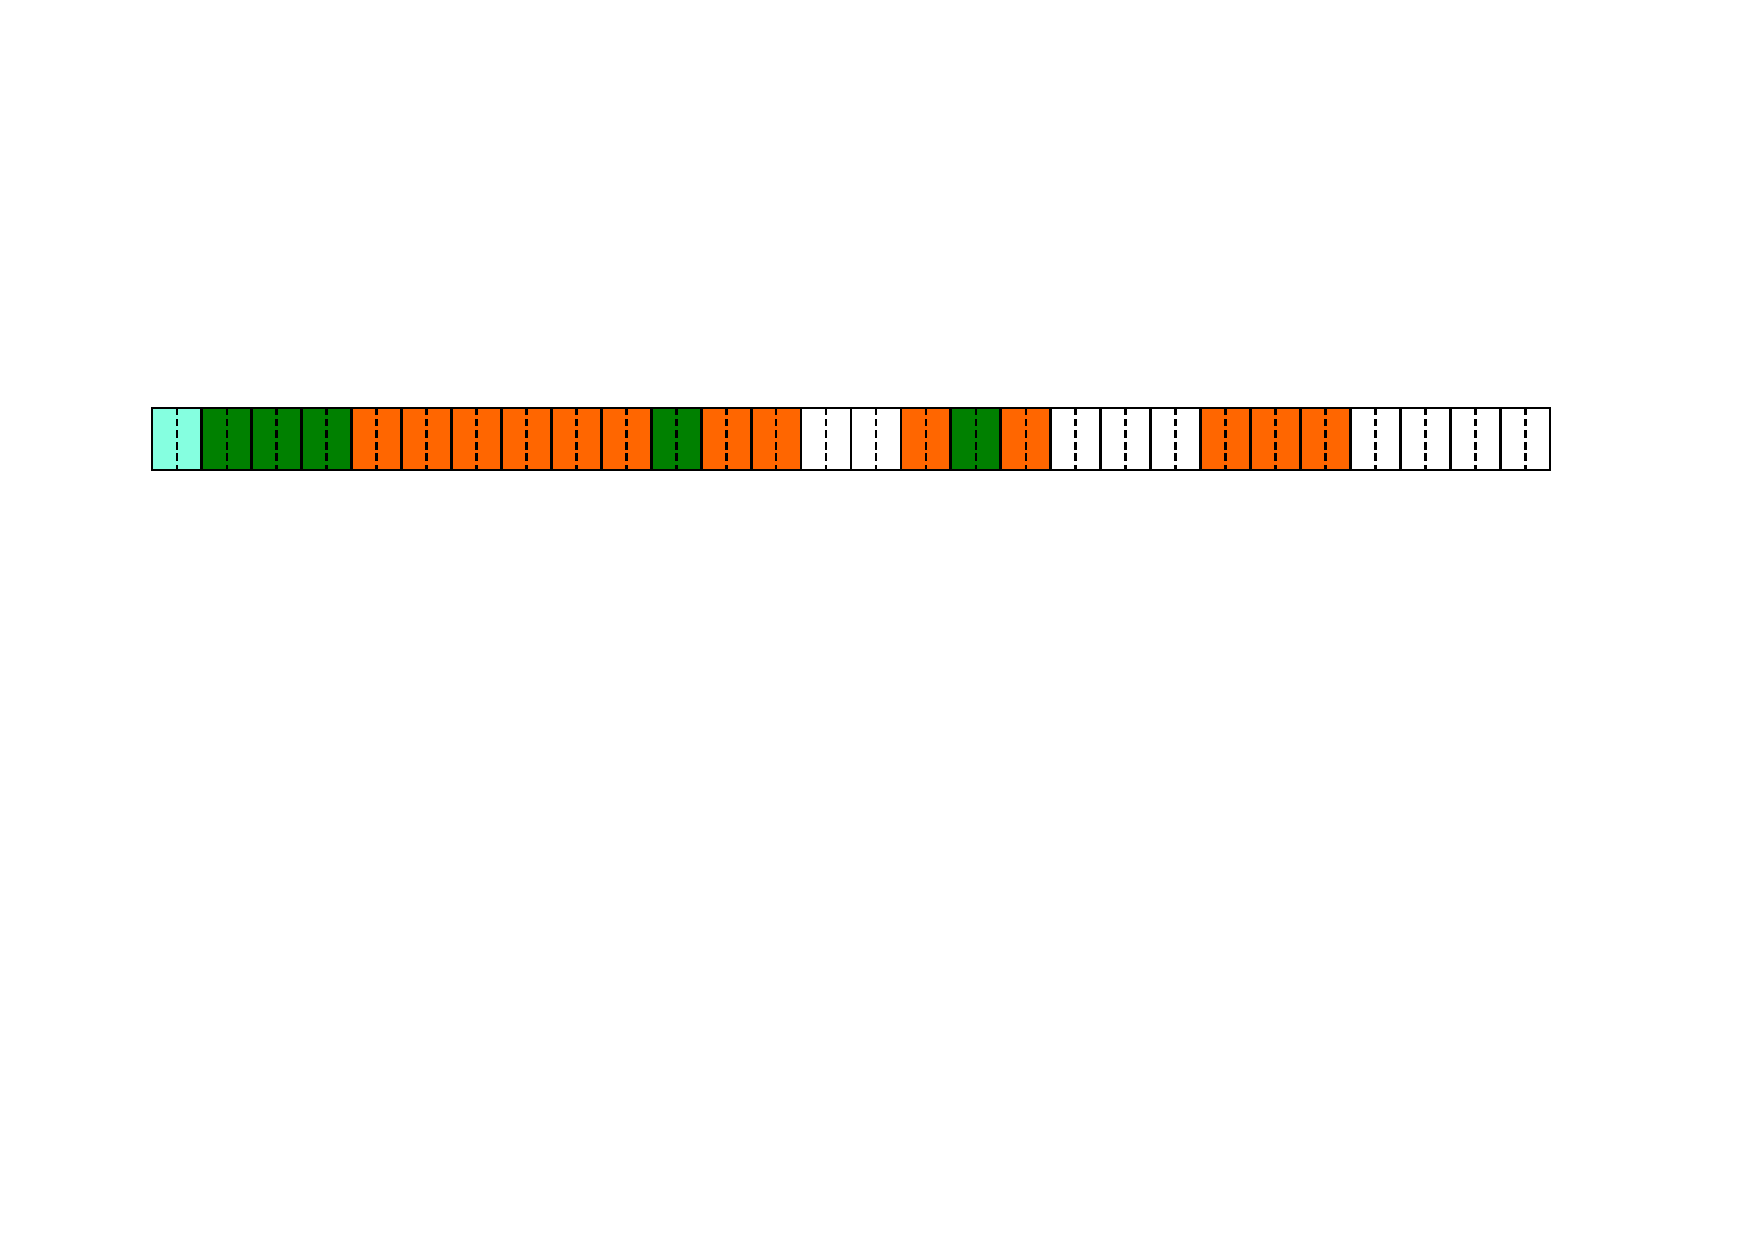
\includegraphics[width=\textwidth]{img/files-1.pdf}
    \caption{A cluster can be seen visually as an array. In this image, for example, we've shown three types of cluster: metadata fixed position (azure), metadata variable position (green), file data (orange), unused space (white).}
\end{figure}

\newpage

\noindent
The following explanation introduces some basic operations on the files to see what happens inside the disks.
\begin{itemize}
    \item \underline{\textbf{Reading}}. To read a file:
    \begin{enumerate}
        \item Access the metadata, variable position (because it contains the folder structure), to locate its block;
        \item Access the blocks to read the contents of the file.
    \end{enumerate}
    \begin{figure}[!htp]
        \centering
        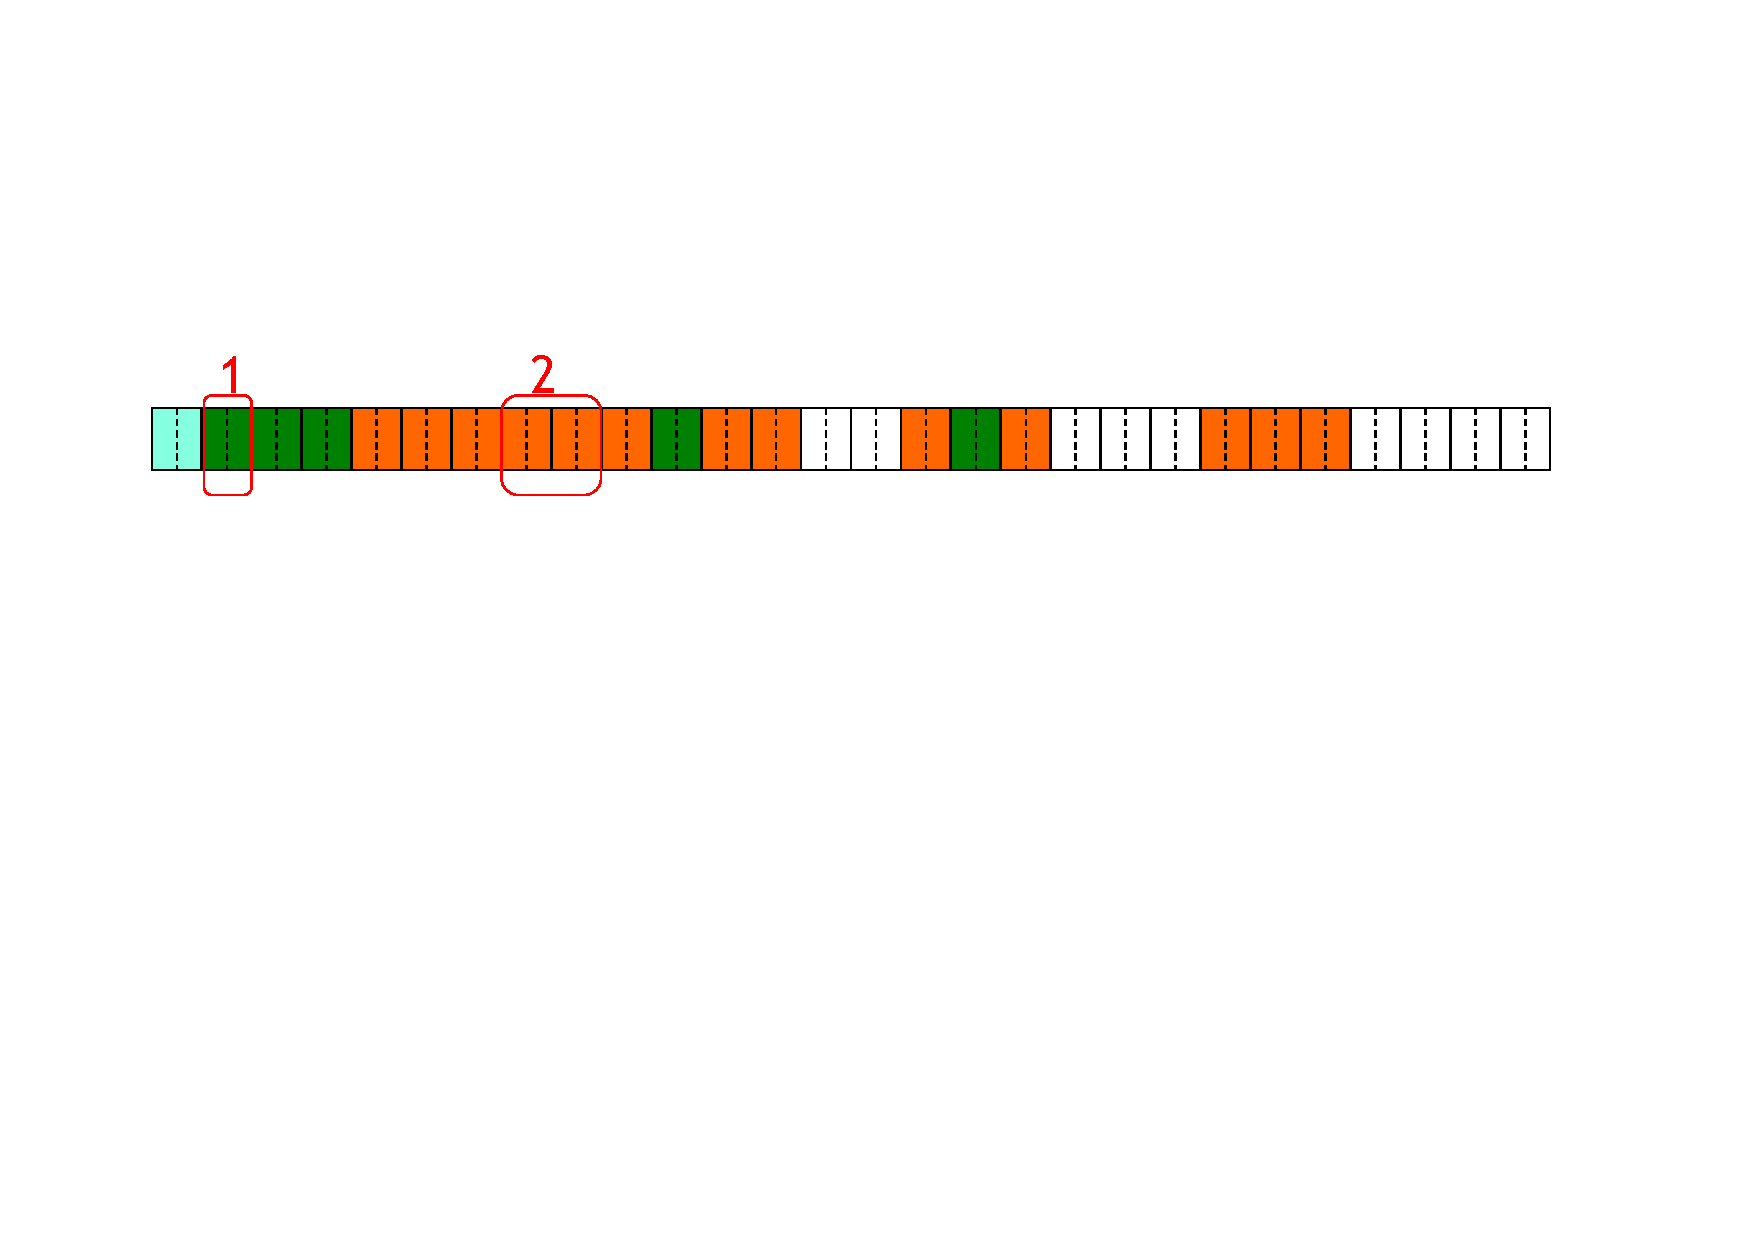
\includegraphics[width=\textwidth]{img/files-2.pdf}
    \end{figure}

    \item \underline{\textbf{Writing}}. To write a file:
    \begin{enumerate}
        \item Access the metadata, variable position (because it contains the folder structure), to find free space.
        \item Write the data in the allocated blocks (cluster type: unused space).        
    \end{enumerate}
    \begin{figure}[!htp]
        \centering
        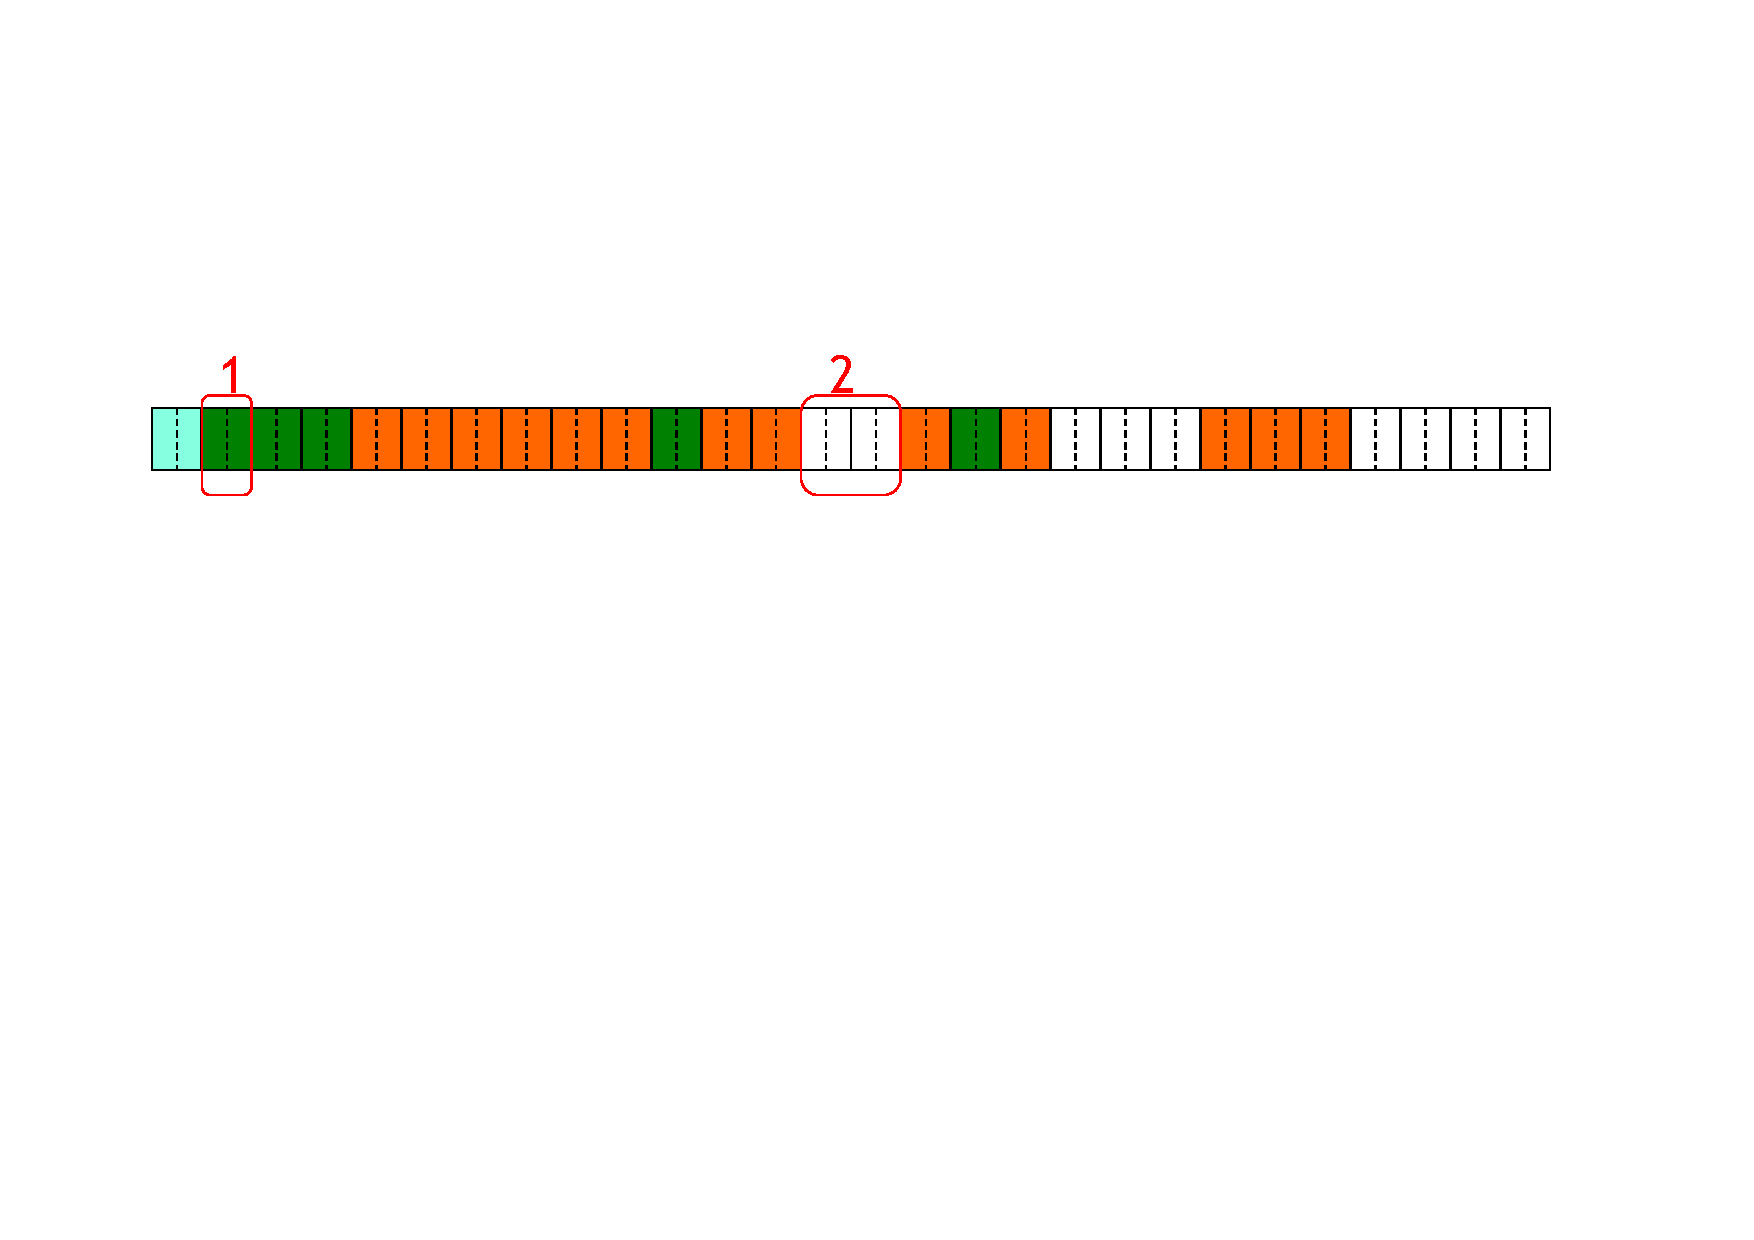
\includegraphics[width=\textwidth]{img/files-3.pdf}
    \end{figure}

    Since the \emph{file system can only access clusters}, the \textbf{actual space taken up by a file on a disk is always a multiple of the cluster size}. Given:
    \begin{itemize}
        \item $s$, the \emph{file size}
        \item $c$, the \emph{cluster size}
    \end{itemize}
    Then the \definition{actual size on the disk $a$} can be calculated as:
    \begin{equation}
        a = \mathrm{ceil}\left(\dfrac{s}{c}\right) \times c
    \end{equation}
    Where $\mathrm{ceil}$ rounds a number \underline{up} to the nearest integer. It's also possible to calculate the \textbf{amount of disk space wasted by organising the file into clusters} (\definition{wasted disk space $w$}):
    \begin{equation}
        w = a - s
    \end{equation}
    A formal way to refer to wasted disk space is \definition{internal fragmentation} of files.
    \newpage
    \begin{examplebox}[: internal fragmentation]
        \begin{itemize}
            \item File size: 27 byte
            \item Cluster size: 8 byte
        \end{itemize}
        The \emph{actual size} on the disk is:
        \begin{equation*}
            a = \mathrm{ceil}\left(\dfrac{27}{8}\right) \cdot 8 = \mathrm{ceil}\left(3.375\right) \cdot 8 = 4 \cdot 8 = 32 \text{ byte}
        \end{equation*}
        And the internal fragmentation $w$ is:
        \begin{equation*}
            w = 32 - 27 = 5 \text{ byte}
        \end{equation*}
    \end{examplebox}

    \item \underline{\textbf{Deleting}}. To delete a file:
    \begin{enumerate}
        \item Just update the metadata, variable position (because it contains the folder structure), to say that the blocks where the file was stored are no longer used by the OS.
    \end{enumerate}
    \textbf{Deleting a file never actually deletes the data on the disk}: if a new file is written to the same clusters, the old data is replaced by the new.
    \begin{figure}[!htp]
        \centering
        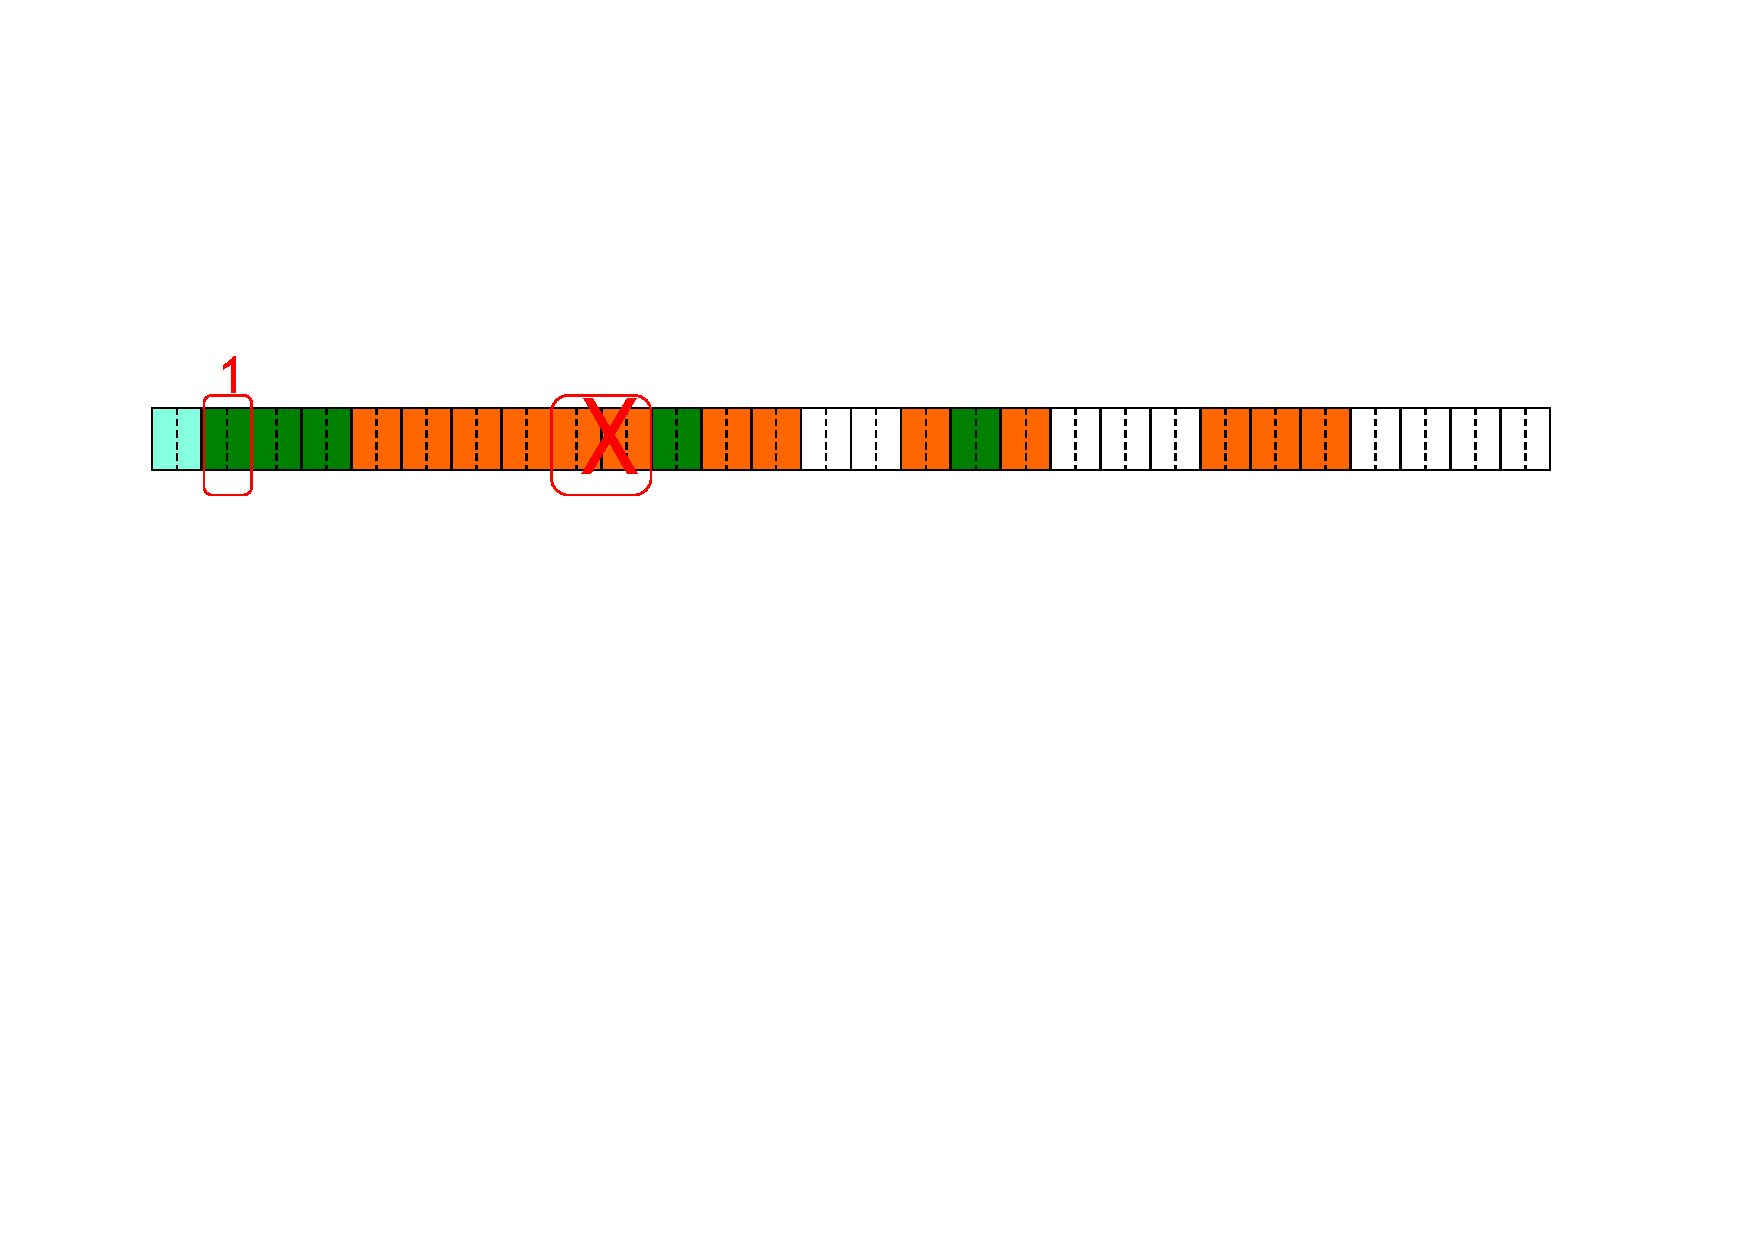
\includegraphics[width=\textwidth]{img/files-4.pdf}
    \end{figure}
    
    \item \underline{\textbf{External fragmentation}}. As the disk's life evolves, there might \textbf{not be enough space to store a file contiguously}.
    
    In this case, the file is split into smaller chunks and inserted into the free clusters spread over the disk.
    
    The effect of \textbf{splitting a file into non-contiguous clusters} is called \definition{external fragmentation}.
    \begin{figure}[!htp]
        \centering
        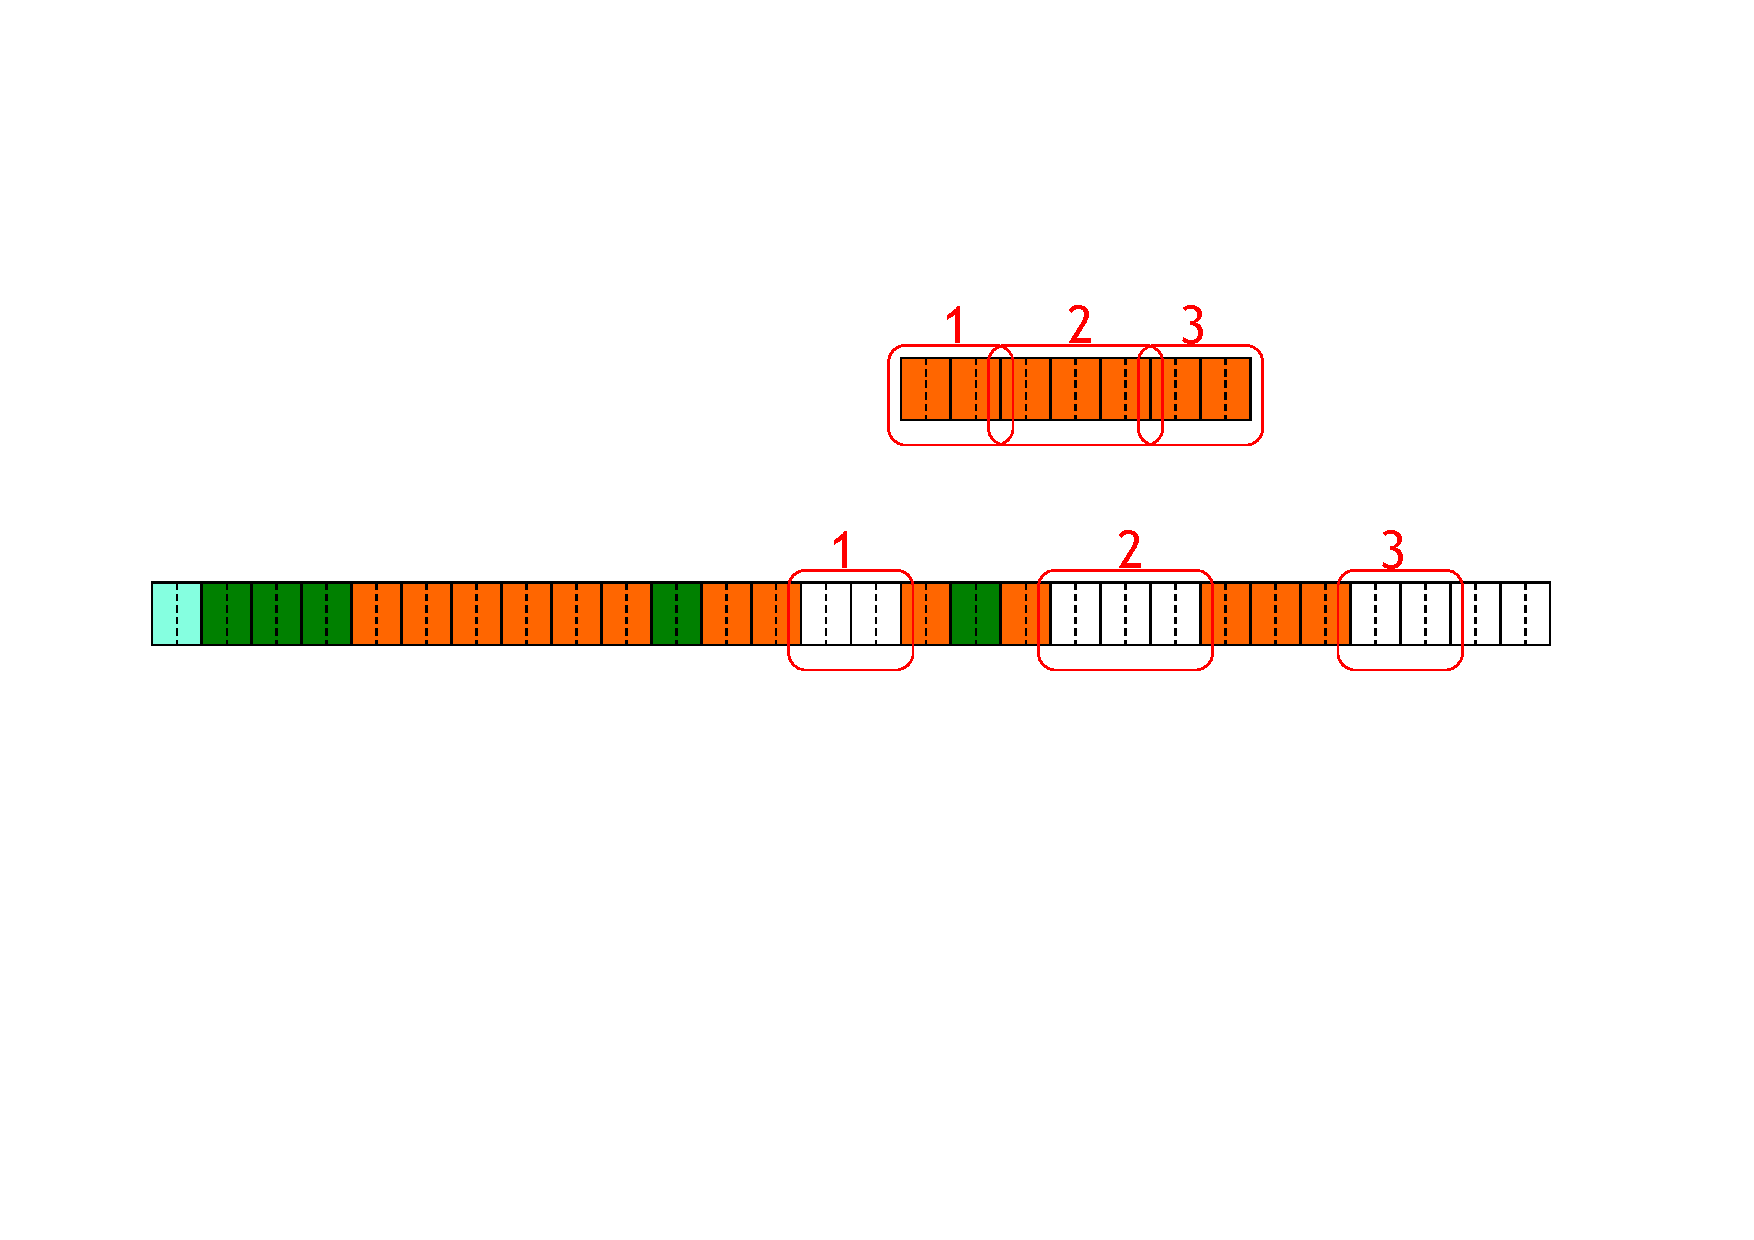
\includegraphics[width=\textwidth]{img/files-5.pdf}
    \end{figure}
\end{itemize}

\newpage

\paragraph{HDD}

A \definition{Hard Disk Drive (HDD)} is a \textbf{data storage device that uses rotating disks (platters) coated with magnetic material}.

\highspace
\textbf{Data is read randomly}, meaning individual data blocks can be stored or retrieved in any order rather than sequentially.

\highspace
An HDD consists of one or more rigid (\emph{hard}) rotating disks (platters) with magnetic heads arranged on a moving actuator arm to read and write data to the surfaces.

\begin{figure}[!htp]
    \centering
    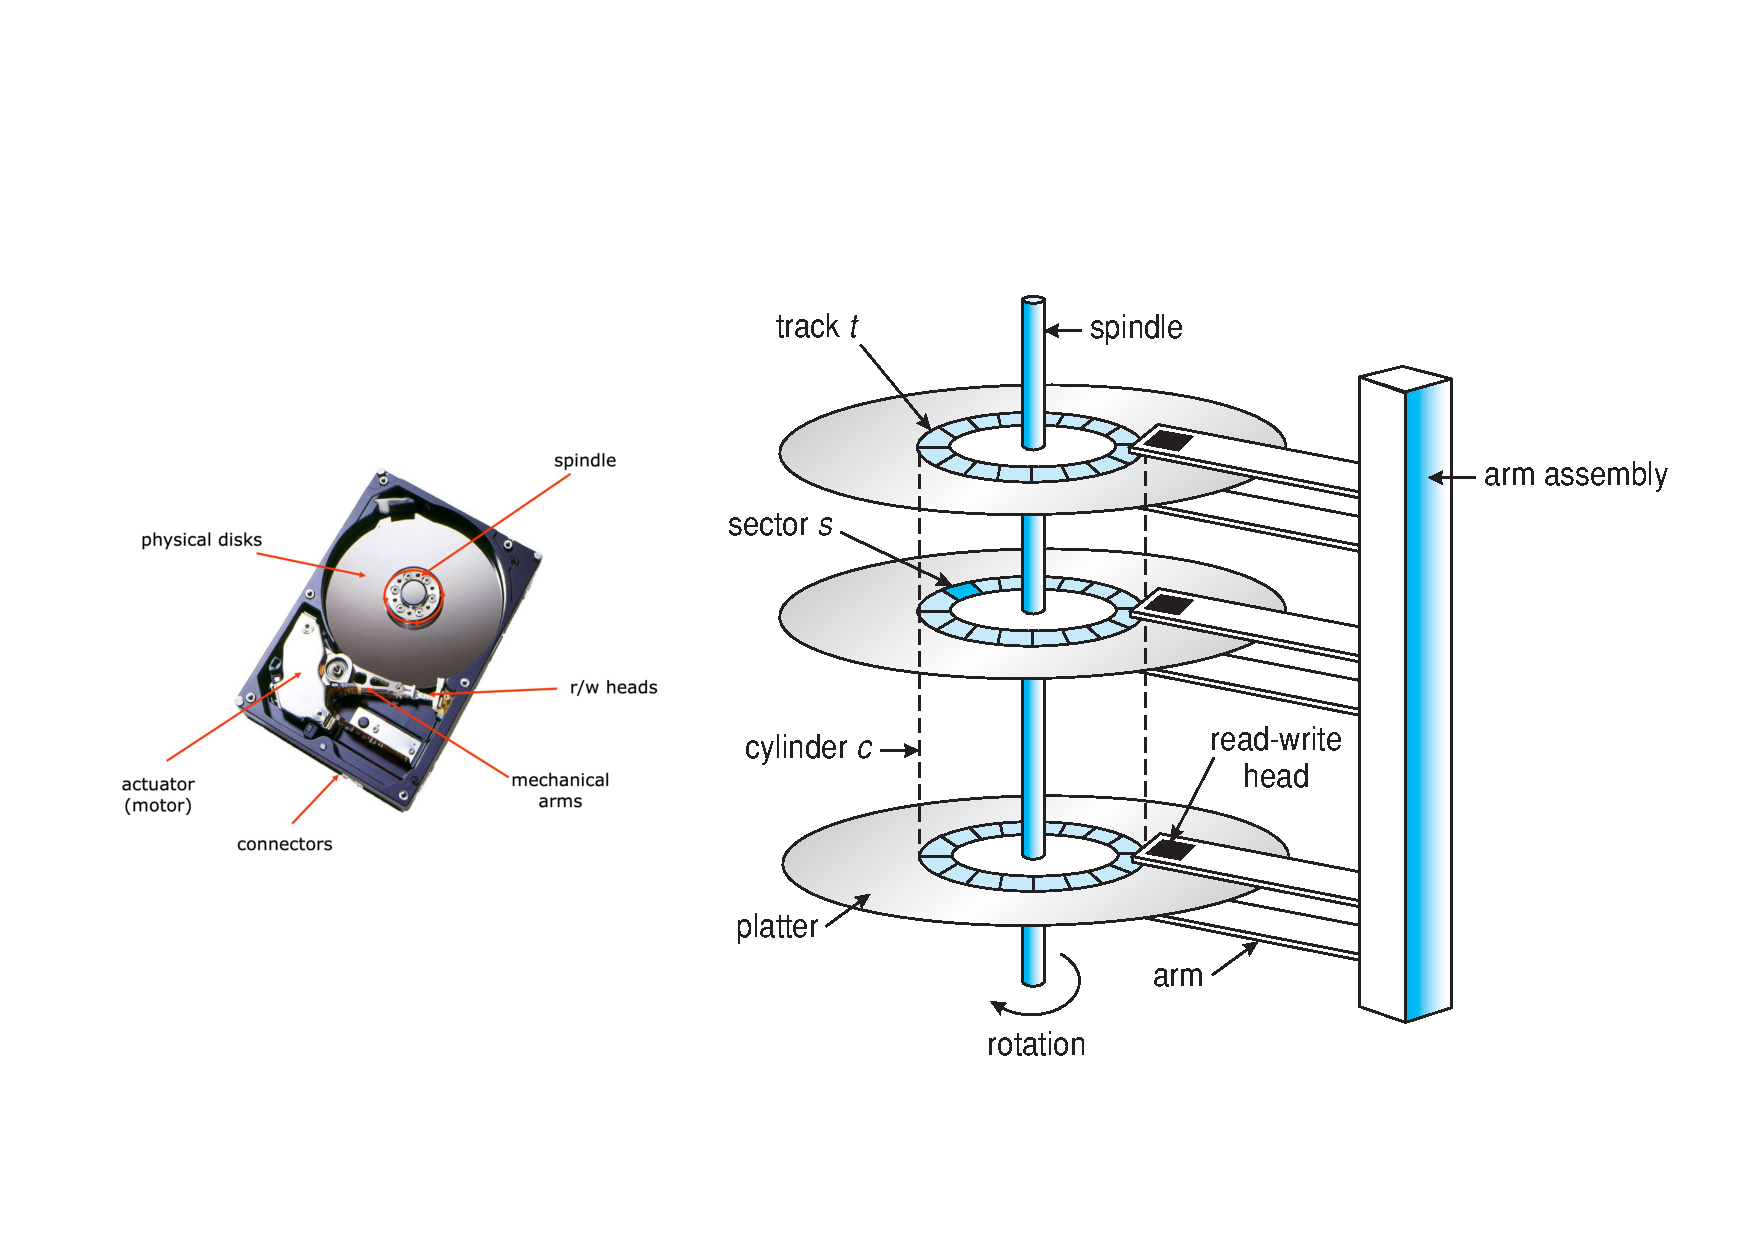
\includegraphics[width=\textwidth]{img/files-6.pdf}
    \caption{Hard Drive Disk anatomy.}
\end{figure}

\noindent
Externally, hard drives expose a large number of \textbf{sectors} (blocks):
\begin{itemize}
    \item Typically, 512 or 4096 bytes.
    \item Individual \textbf{sector writes} are \textbf{atomic}.
    \item Multiple sectors write it may be interrupted (\definition{torn write}\footnote{Torn writes happen when only part of a multi-sector update is written successfully to disk.}).
\end{itemize}
The geometry of the drive:
\begin{itemize}
    \item The sectors are arranged into \textbf{tracks}.
    \item A \textbf{cylinder} is a particular track on multiple platters.
    \item Tracks are arranged in concentric circles on \textbf{platters}.
    \item A disk may have multiple double-sided platters.
\end{itemize}
The \textbf{driver motor spins the platters at a constant rate}, measured in \definition{Revolutions Per Minute (RPM)}.

\newpage

\begin{figure}[!htp]
    \centering
    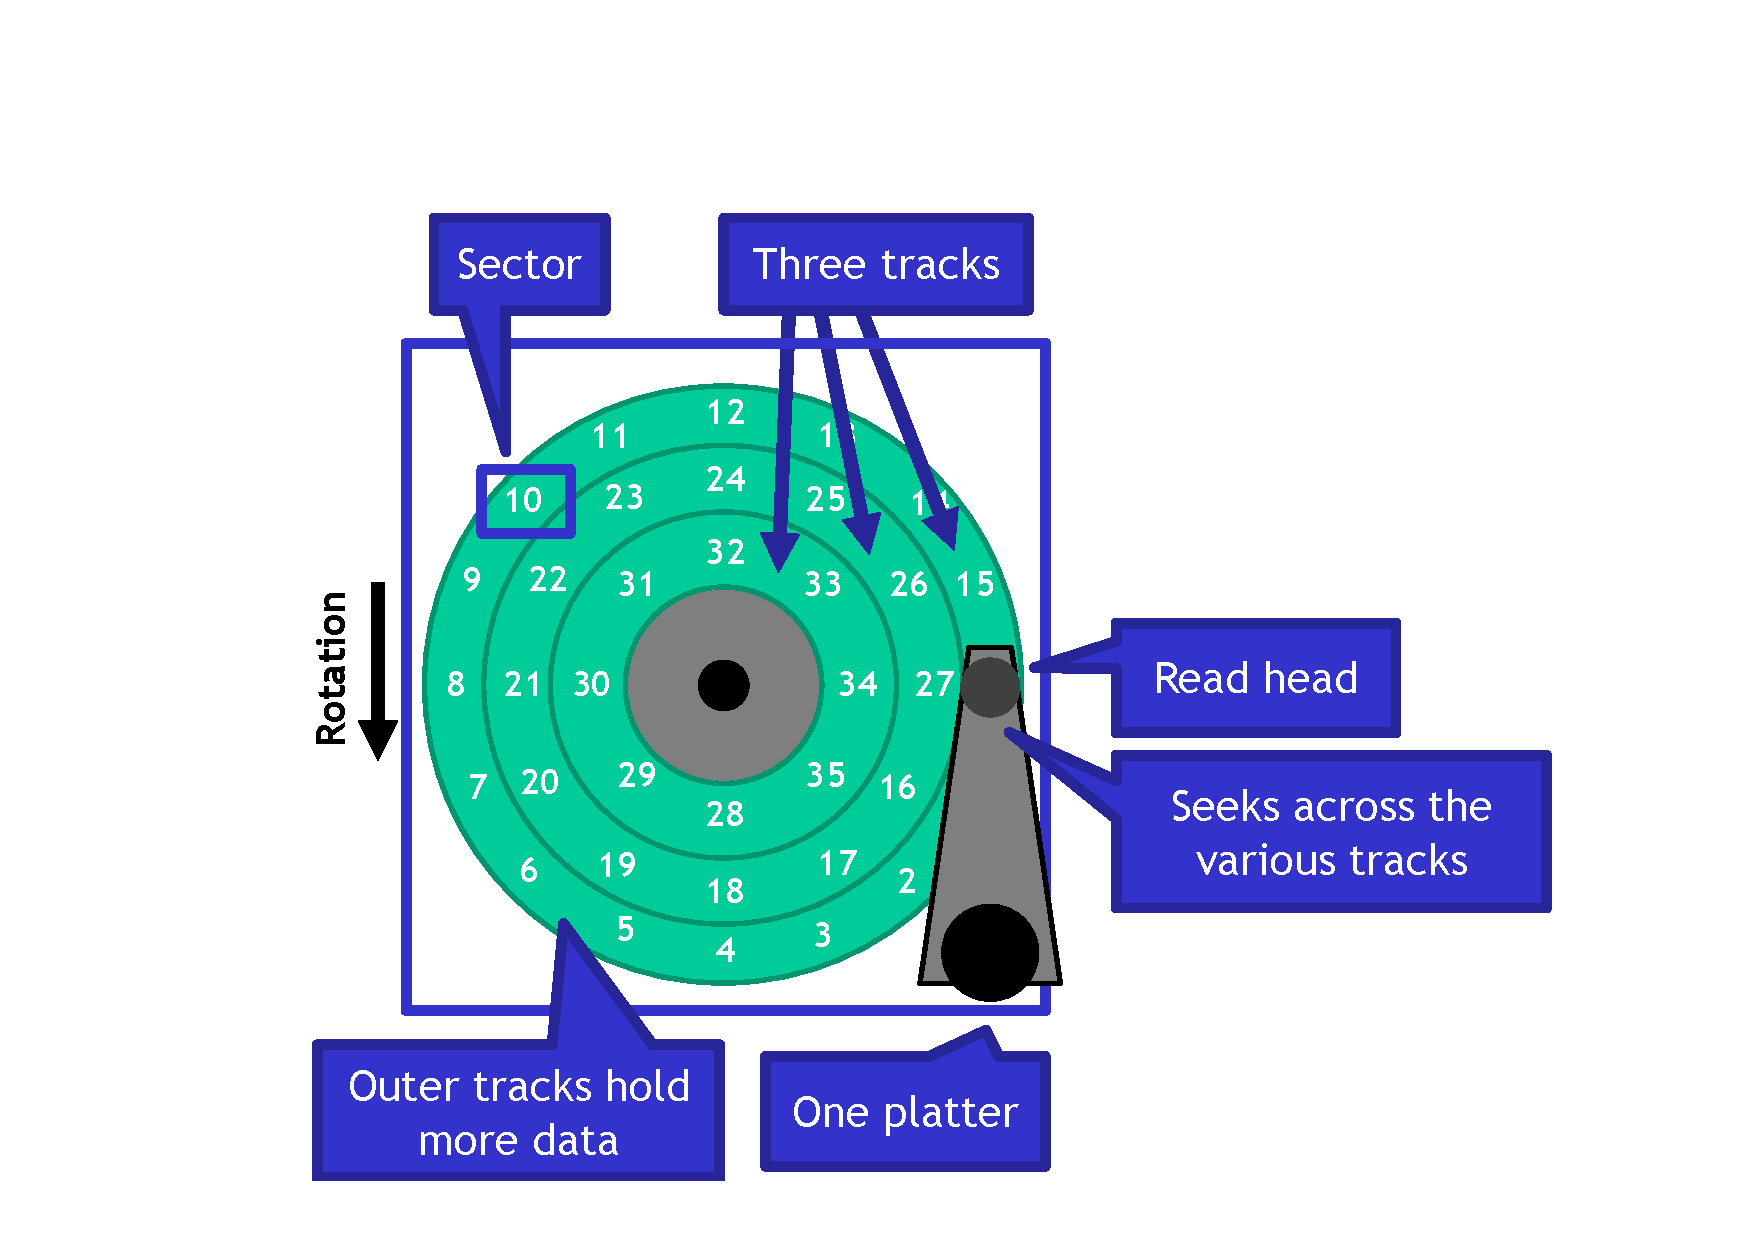
\includegraphics[width=.8\textwidth]{img/files-7.pdf}
    \caption{Example of HDD geometry.}
\end{figure}

Given the architecture of the HDD, there are \textbf{four types of delay}:
\begin{itemize}\label{four types of hdd delay}
    \item \definition{Rotational Delay} is the \textbf{time to rotate the desired sector to the read head}, and it's related to RPM.
    \item \definition{Seek Delay} is the \textbf{time to move the read head to a different track}.
    \item \definition{Transfer time} is the \textbf{time to read or write bytes}.
    \item \definition{Controller Overhead} is the \textbf{overhead for the request management}.
\end{itemize}
In order to reduce the delay in the HDD, the companies use a high-speed and tiny memory (8, 16 or 32 MB) called \definition{cache} (also called \definition{track buffer}). The cache is used when there is a:
\begin{itemize}
    \item \definition{Read caching}. It reduces read delays due to seeking and rotation.
    
    \item \definition{Write caching}. It is divided into two different implementations:
    \begin{itemize}
        \item \definition{Write Back cache}: the drive reports that writes are complete after they have been cached. The disadvantage is that it has an inconsistent state if the power goes off before the write-back event.
        
        \item \definition{Write Through cache}: the drive reports that writes are complete after they have been written to disk.
    \end{itemize}
\end{itemize}
So, the \textbf{caching helps improve disk performance}. The critical idea under caching is that if there is a \textbf{queue of requests to the disk, they can be reordered to improve performance}. The estimation of the request length is feasible, knowing the position of the data on the disk.

\newpage

\noindent
There are several \textbf{scheduling algorithms}:
\begin{itemize}
    \item \definition{First Come, First Serve (FCFC)}. It is the most basic scheduler, serving requests in order. The \emph{\textbf{disadvantage}} is that there is much time spent seeking.

    \item \definition{Shortest Seek Time First (SSTF)}. It is primary purpose is to minimize seek time by always selecting the block with the shortest seek time. The \textbf{\emph{advantage}} is that it is optimal and can be easily implemented. The main \emph{\textbf{disadvantage}} is that it is prone to starvation.

    \item \definition{SCAN}, otherwise known as the Elevator Algorithm. The head sweeps across the disk, servicing requests in order. The \textbf{\emph{advantage}} is that it performs reasonably well and does not suffer starvation. The \emph{\textbf{disadvantage}} is that the average access times are higher for requests at high and low addresses.

    \item \definition{C-SCAN (Circular SCAN)}. It is like the SCAN algorithm, but only service requests in one direction. The \textbf{\emph{advantage}} is fairer than SCAN. However, the \emph{\textbf{disadvantage}} is that it has worse performance than SCAN.

    \item \definition{C-LOOK}. It is a C-SCAN variant that peeks at the upcoming addresses in the queue. The head only goes as far as the last request.
\end{itemize}

\newpage

\paragraph{SSD}

The \definition{solid-state drive (SSD)} does not have mechanical or moving parts like an HDD. It is built out of transistors (like memory and processors). It has higher performance than HDD.

\highspace
It stores bits in cells. Each cell can have:
\begin{itemize}
    \item Single-Level Cell (SLC), a single bit per cell.
    \item Multi-Level Cell (MLC), two bits per cell.
    \item Triple-Level Cell (TLC), three bits per cell.
    \item And so on... QLC, PLC, etcetera.
\end{itemize}
Internally, the SSD has a lot of NAND flashes, which are organized into Pages and Blocks. Some terminology:
\begin{itemize}
    \item A \definition{Page} contains \textbf{multiple logical block} (e.g. 512 B - 4 KB) \textbf{addresses} (LBAs). It is the \textbf{smallest unit that can be read/written}. It is a sub-unit of an erase block and consists of the number of bytes which can be read/written in a single operation. The states of each page are:
    \begin{itemize}
        \item \index{Erased Page}\index{Empty Page} \textbf{Empty} (\texttt{ERASED}): it does not contain data.
        \item \index{Invalid Page}\index{Dirty Page} \textbf{Dirty} (\texttt{INVALID}): it contains data, but this data is no longer in use (or never used).
        \item \index{In Use Page}\index{Valid Page} \textbf{In use} (\texttt{VALID}): the page contains data that can be read.
    \end{itemize}

    \item A Block (or \definition{Erase Block}) typically consists of \textbf{multiple pages} (e.g. 64) with a total capacity of around 128-256 KB. It is the \textbf{smallest unit that can be erased}.
\end{itemize}

\highspace
When passing from the HDD to SDD, there is a problem known as Write Amplification (WA). \definition{Write amplification (WA)}\label{Write amplification (WA)} is an \textbf{undesirable phenomenon associated with flash memory and solid-state drives (SSDs)} where the actual amount of information physically written to the storage media is a multiple of the logical amount intended to be written.

\begin{examplebox}
    Given a hypothetical SSD:
    \begin{itemize}
        \item Page Size: 4 KB
        \item Block Size: 5 Pages
        \item Drive Size: 1 Block
        \item Read Speed: 2 KB/s
        \item Write Speed: 1 KB/s
    \end{itemize}
    Let us write a 4 KB text file to the brand-new SSD. The overall writing time is 4 seconds (write speed $\times$ file dimension, 1 KB/s $\times$ 4 KB).

    \newpage

    Now, let us write an 8 KB picture file for the almost brand-new SSD; thankfully, there is space. The overall Writing time is 8 seconds, and the calculation is the same as above.

    \begin{center}
        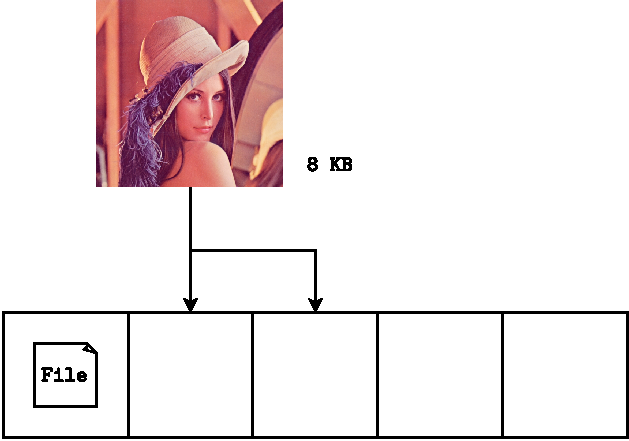
\includegraphics[width=.7\textwidth]{img/SSD-1.pdf}
    \end{center}
    Now, consider that the first file inserted on the first page is unnecessary.

    \highspace
    Finally, let's write a 12 KB pic to the SSD. Theoretically, the image should take 12 seconds. However, it is wrong! The SSD has only two empty pages and one dirty page (invalid). Then, the operations are:
    \begin{enumerate}
        \item Read block into cache.
        \item Delete page from cache (set dirty page).
        \item Write a new picture into the cache.
        \item Erase the old block on the SSD.
        \item Write cache to SSD.
    \end{enumerate}
    The OS only thought it was writing 12 KBs of data when the SSD had to read 8 KBs (2 KB/s) and then write 20 KBs (1 KB/s), the entire block. The writing should have taken 12 seconds but took 4 + 20 = 24 seconds, resulting in a write speed of 0.5 KB/s, not 1 KB/s.
\end{examplebox}

\noindent
A direct mapping between Logical and Physical pages is not feasible inside the SSD. Therefore, each SSD has an FTL component that makes the SSD \emph{look like an HDD}.

\highspace
The \definition{Flash Translation Layer (FTL)} is placed in the hierarchy between the \textbf{File System} and \textbf{Flash Memory}. It aims to do \textbf{three main actions}:
\begin{enumerate}
    \item \textbf{Data Allocation} and \textbf{Address Translation}: It efficiently reduces Write Amplification effects (see page~\pageref{Write amplification (WA)}); the program pages within an erased block in order (from low to high pages), called \definition{Log-Structured FTL}.

    \item \textbf{Garbage collection}: reuse of pages with old data (Dirty/Invalid).

    \item \textbf{Wear levelling}: FTL should spread across the blocks of the flash, ensuring that all of the blocks of the device wear out roughly simultaneously.
\end{enumerate}

\begin{examplebox}[: Log-Structured FTL]
    Assume that a page size is $4$ KB and a block consists of four pages. The write list is (\texttt{Write(pageNumber, value)}):
    \begin{itemize}
        \item \texttt{Write(100, a1)}
        \item \texttt{Write(101, a2)}
        \item \texttt{Write(2000, b1)}
        \item \texttt{Write(2001, b2)}
        \item \texttt{Write(100, c1)}
        \item \texttt{Write(101, c2)}
    \end{itemize}
    The steps are:
    \begin{enumerate}
        \item The initial state is with all pages marked as \texttt{INVALID(i)}:
        \begin{center}
            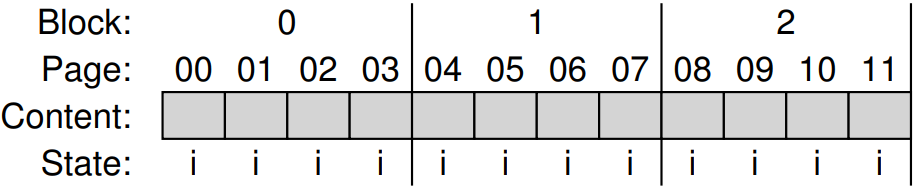
\includegraphics[width=.7\textwidth]{img/log-structured-ftl-1.png}
        \end{center}

        \item Erase block zero:
        \begin{center}
            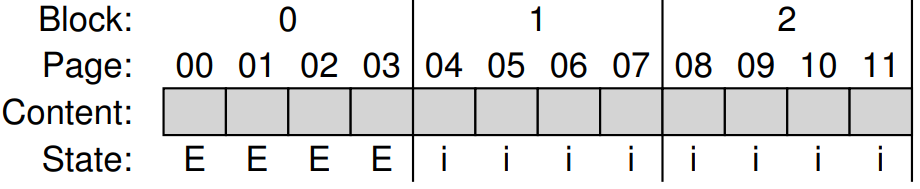
\includegraphics[width=.7\textwidth]{img/log-structured-ftl-2.png}
        \end{center}

        \item Program pages in order and update mapping information (\texttt{Write(100, a1)}):
        \begin{center}
            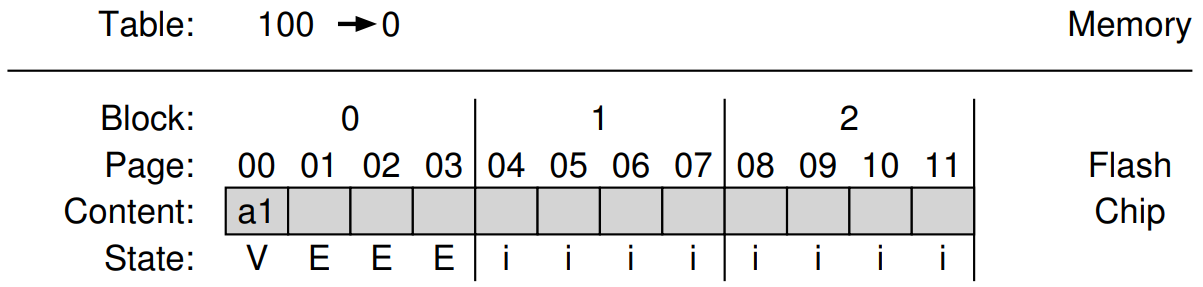
\includegraphics[width=.8\textwidth]{img/log-structured-ftl-3.png}
        \end{center}

        \item After performing four writes (\texttt{Write(100, a1)}, \texttt{Write(101, a2)}, \texttt{Write(2000, b1)}, \texttt{Write(2001, b2)}):
        \begin{center}
            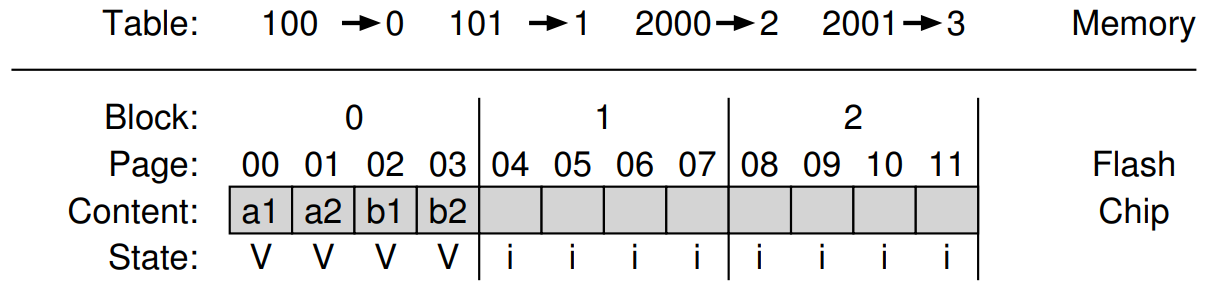
\includegraphics[width=.8\textwidth]{img/log-structured-ftl-4.png}
        \end{center}

        \item After updating $100$ and $101$:
        \begin{center}
            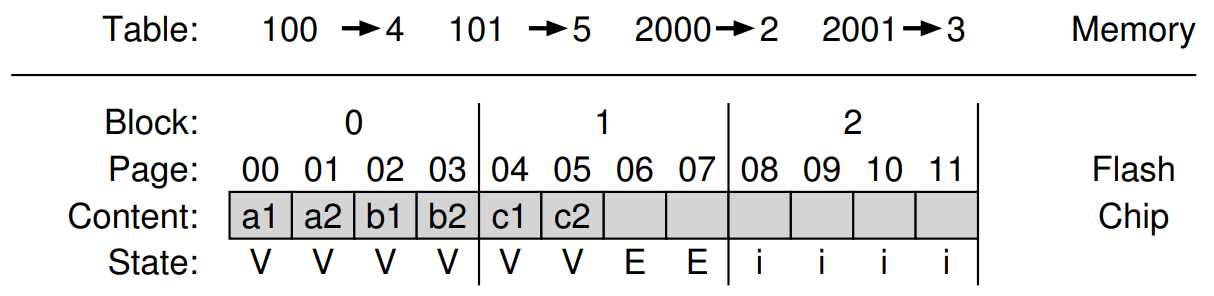
\includegraphics[width=.8\textwidth]{img/log-structured-ftl-5.png}
        \end{center}
    \end{enumerate}
\end{examplebox}

\noindent
When an existing page is updated, then the old data becomes obsolete. The \textbf{old versions of data are called garbage}, and (sooner or later) garbage pages must be reclaimed for new writes to take place.

\highspace
The \definition{Garbage Collection} is the \textbf{process of finding garbage blocks and reclaiming them}. It is a simple process for fully garbage blocks but more complex for partial cases.

\begin{examplebox}[: how garbage collection works]
    The steps are:
    \begin{enumerate}
        \item Update request for existing data:
        \begin{center}
            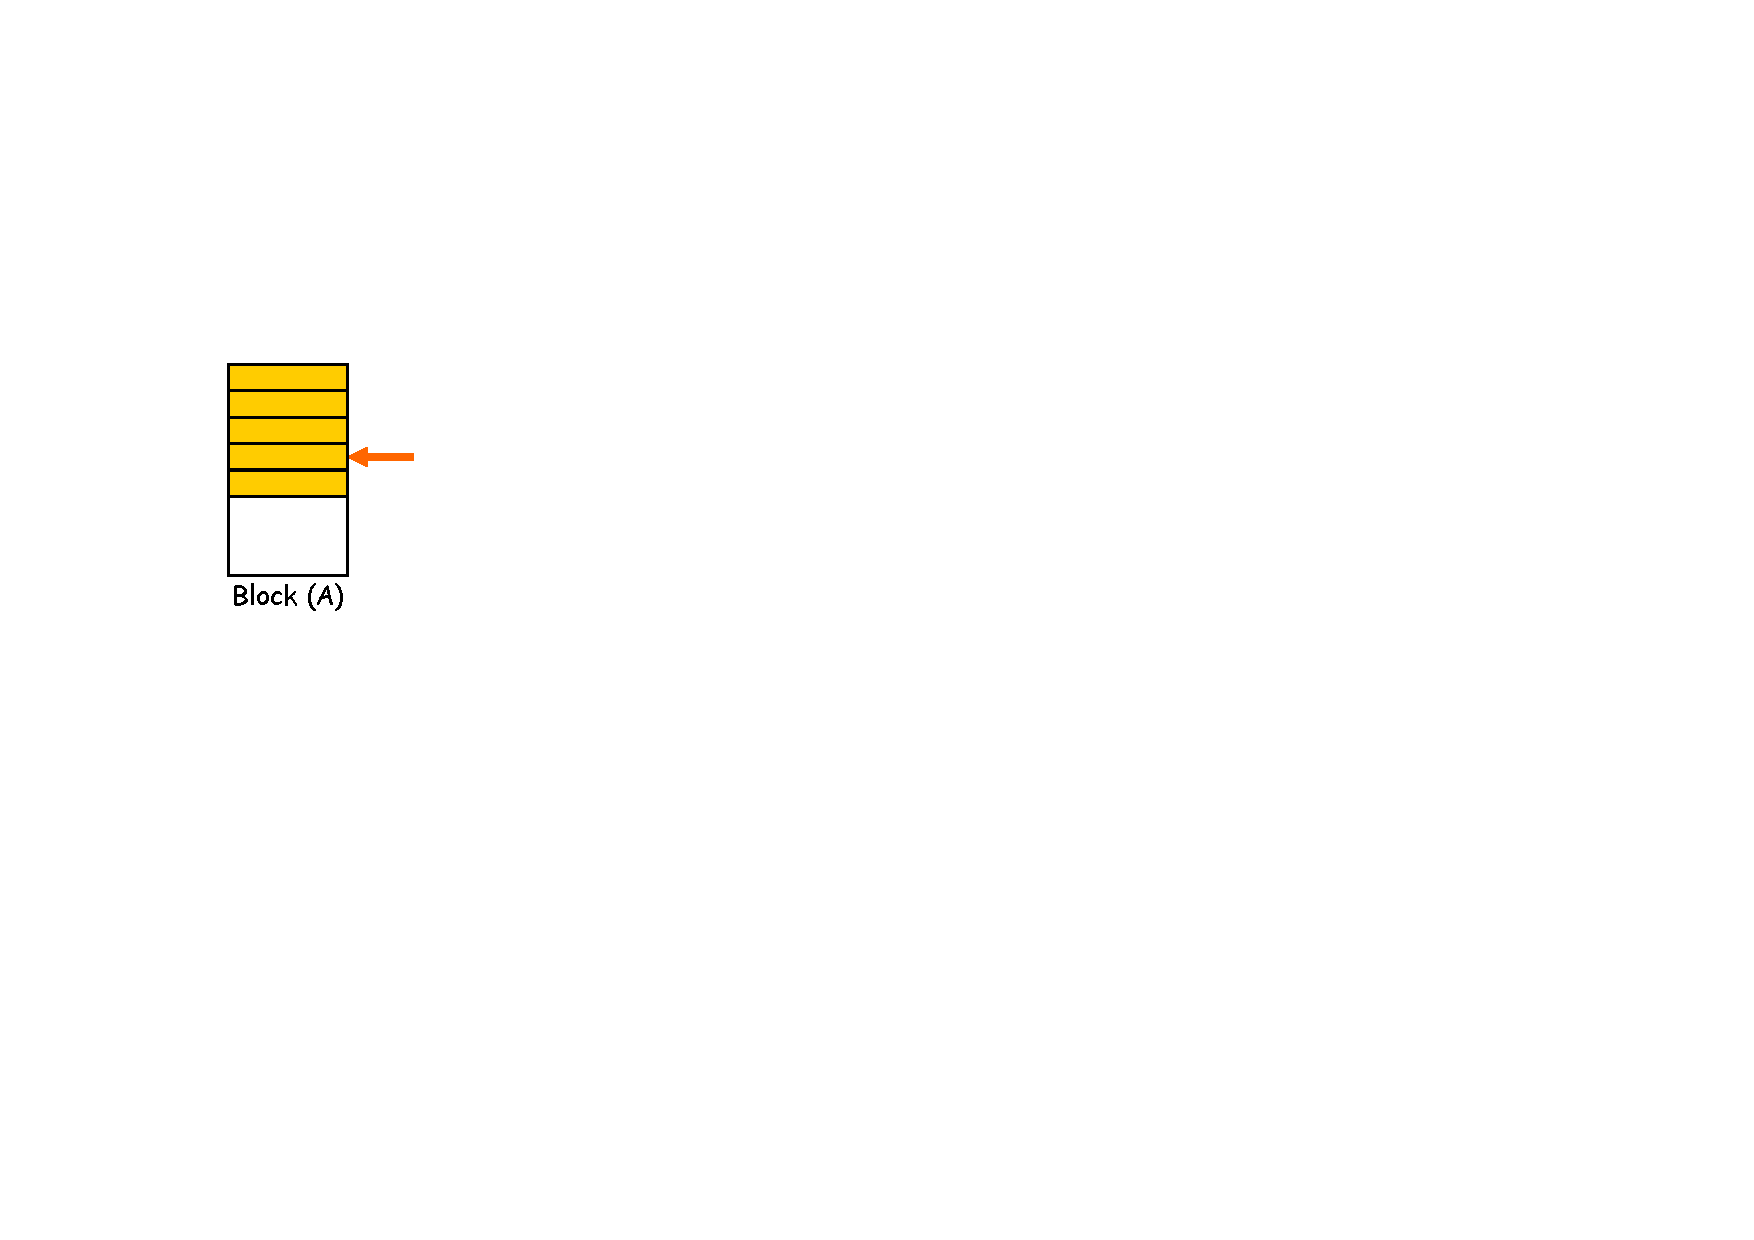
\includegraphics[width=.24\textwidth]{img/garbage-collection-1.pdf}
        \end{center}

        \item Find a free page, and save the new data:
        \begin{center}
            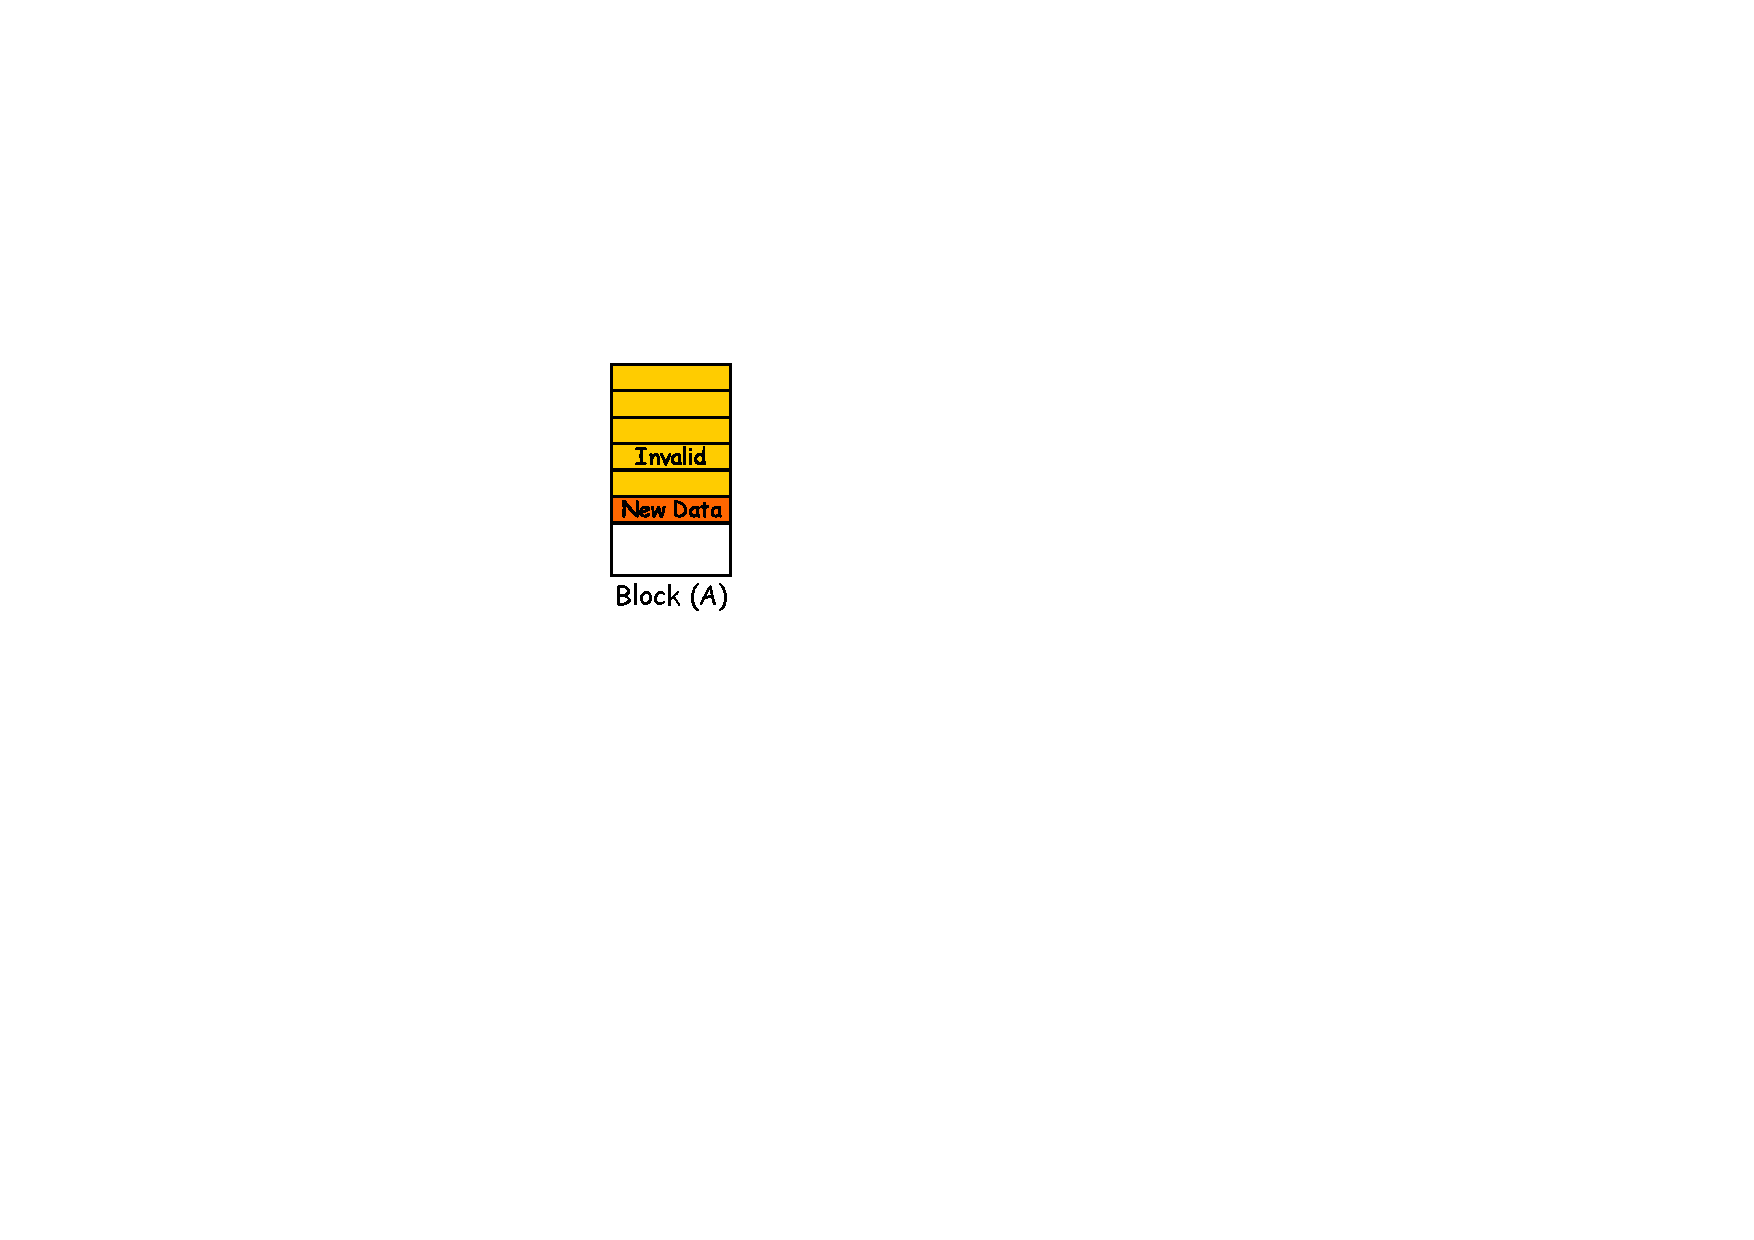
\includegraphics[width=.15\textwidth]{img/garbage-collection-2.pdf}
        \end{center}

        \item This scenario may continue until there are not enough free blocks:
        \begin{center}
            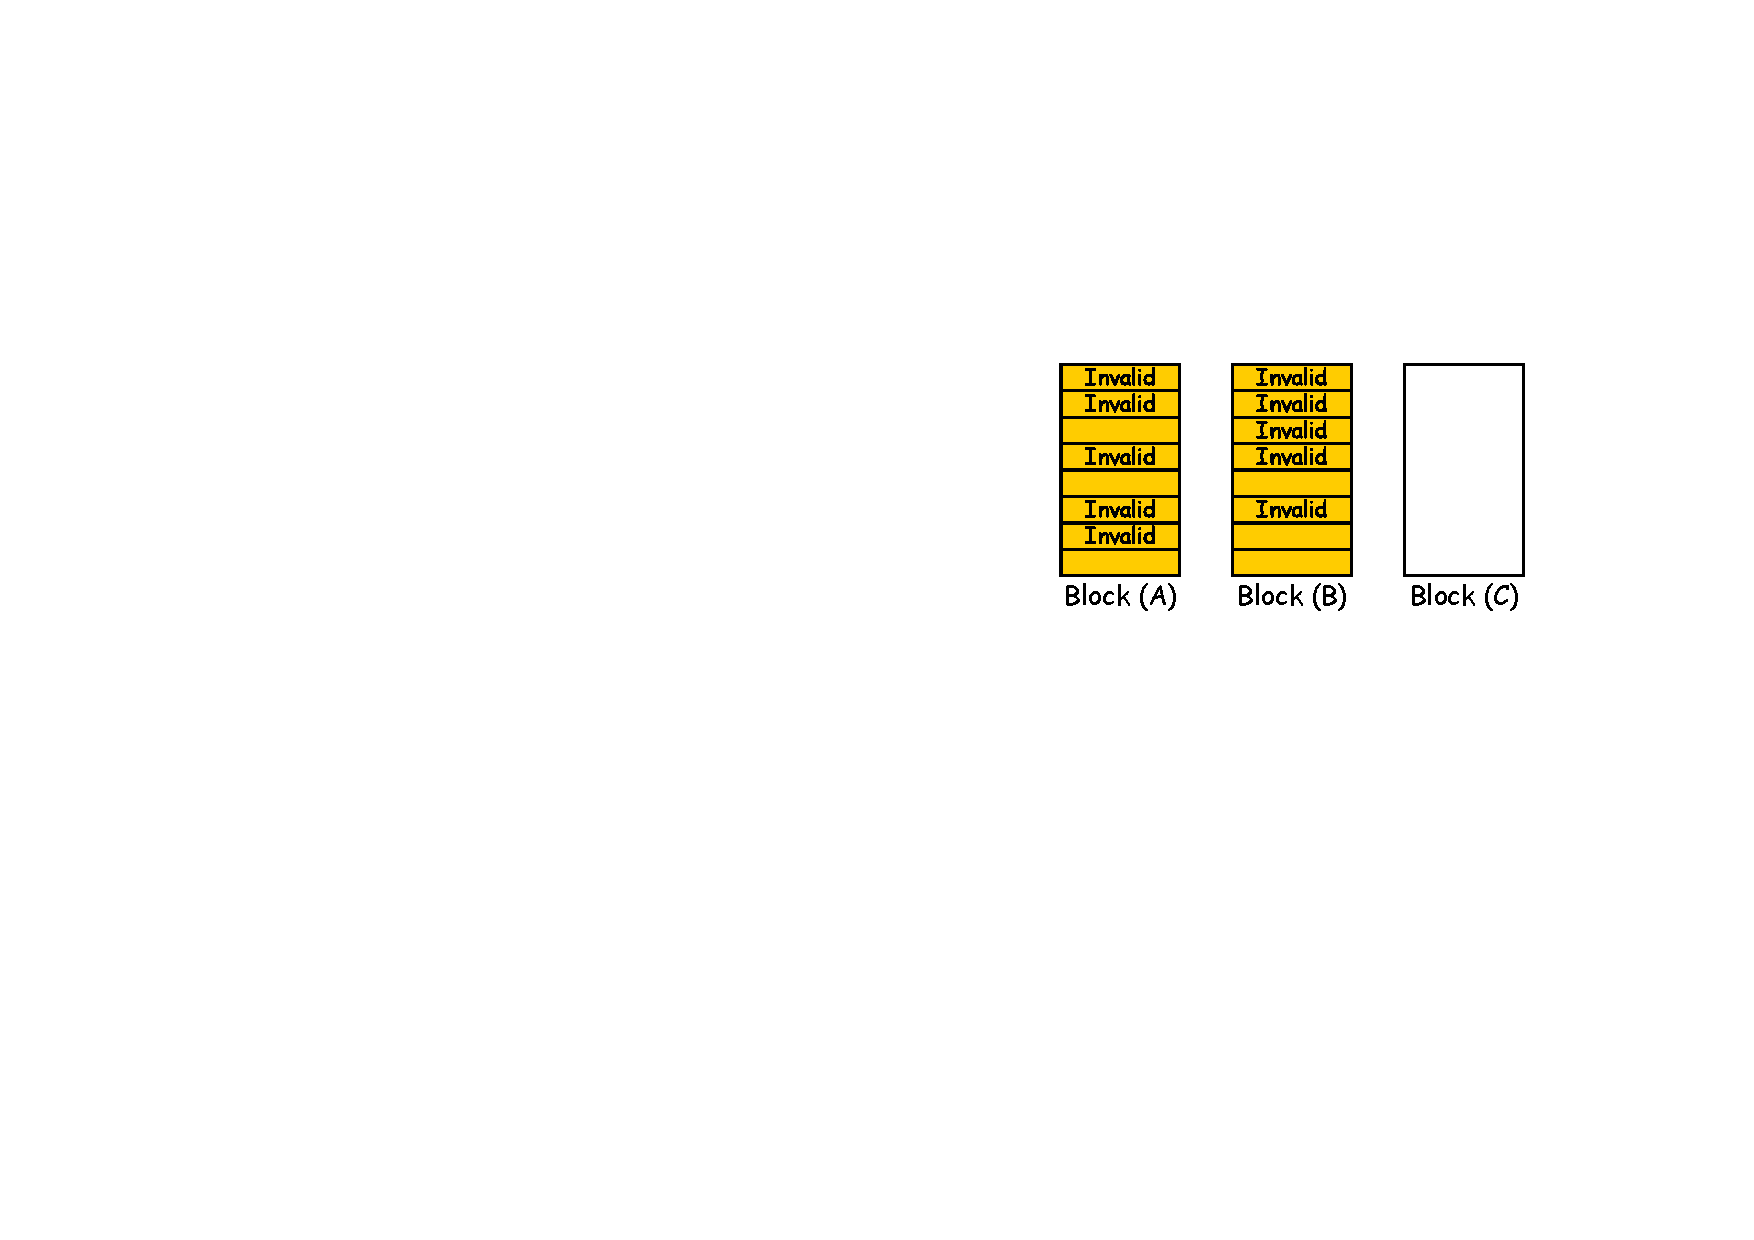
\includegraphics[width=.5\textwidth]{img/garbage-collection-3.pdf}
        \end{center}

        \item Collect valid pages into a free block:
        \begin{center}
            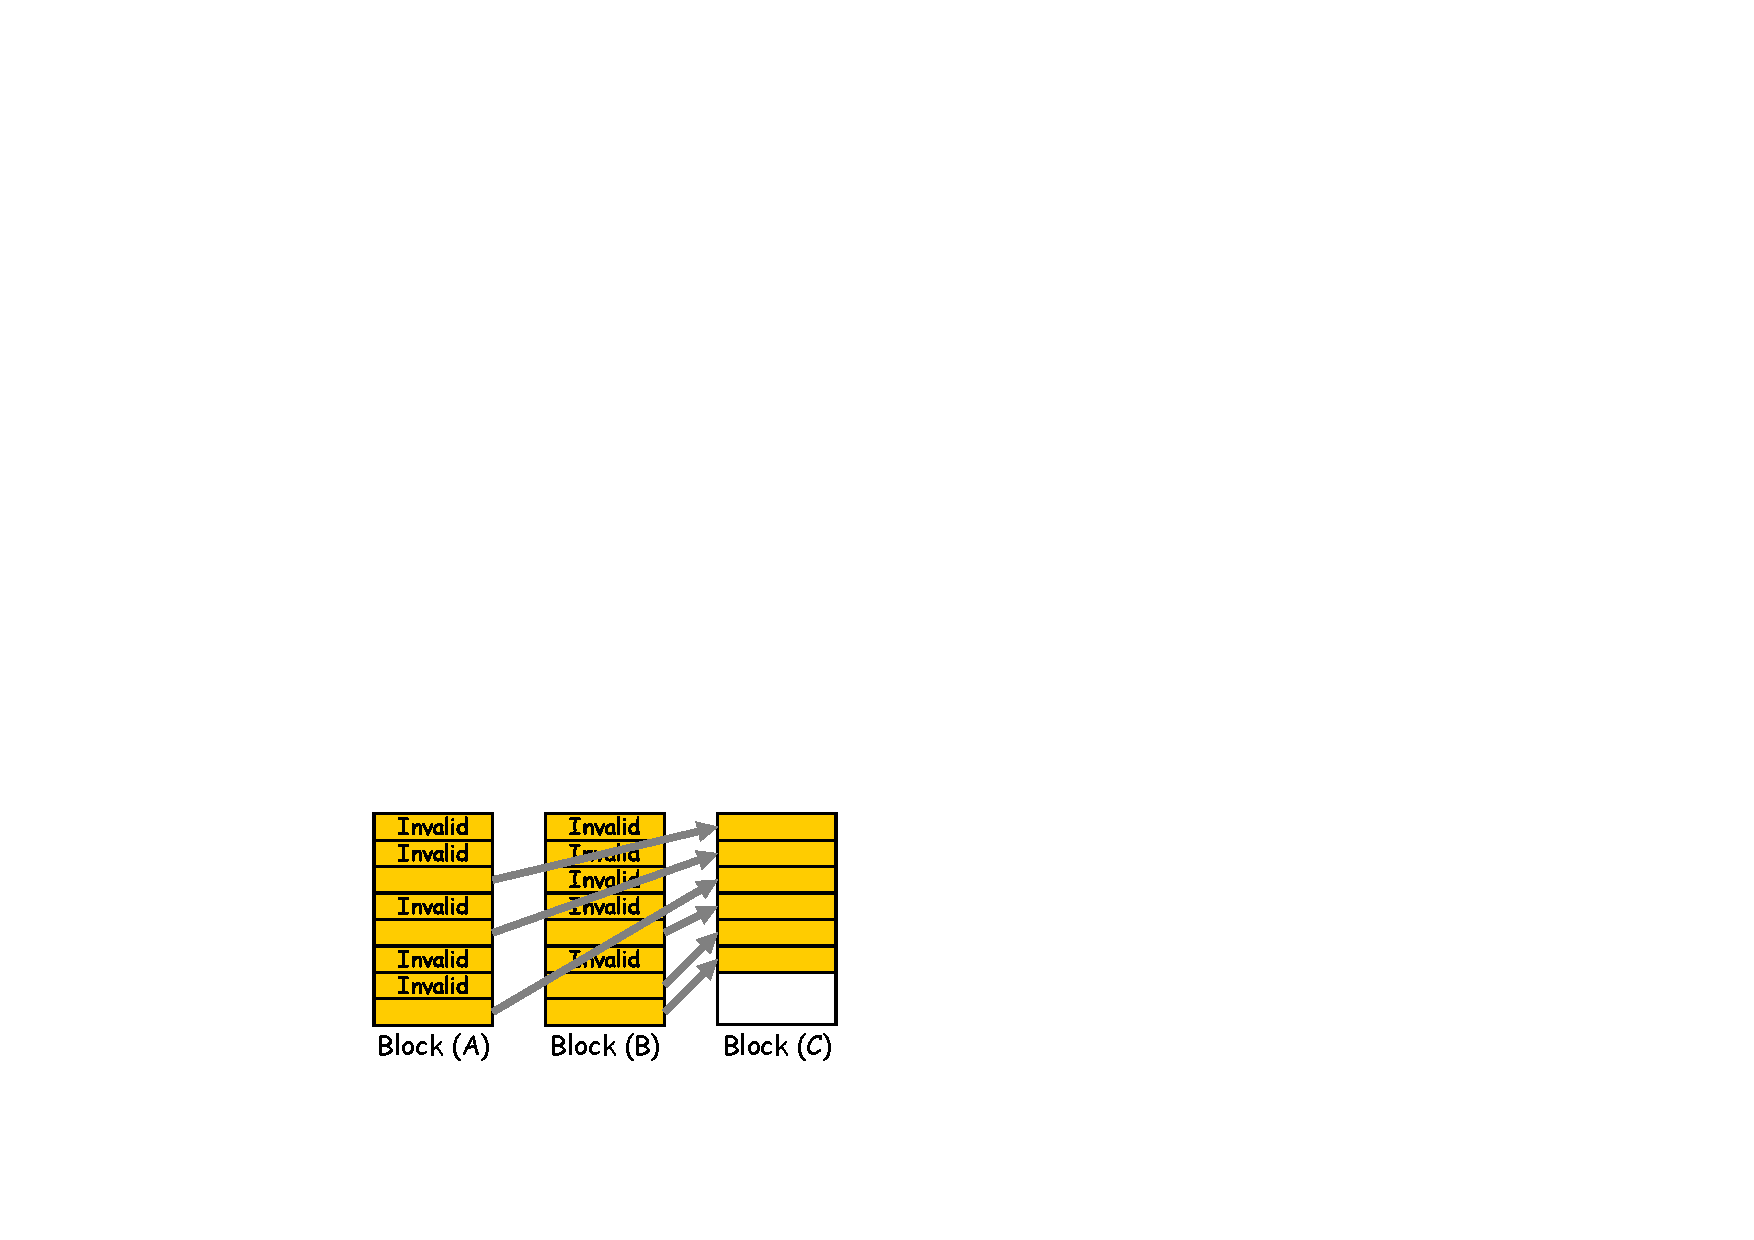
\includegraphics[width=.5\textwidth]{img/garbage-collection-4.pdf}
        \end{center}

        \item Update the map table and erase invalid (obsolete) blocks:
        \begin{center}
            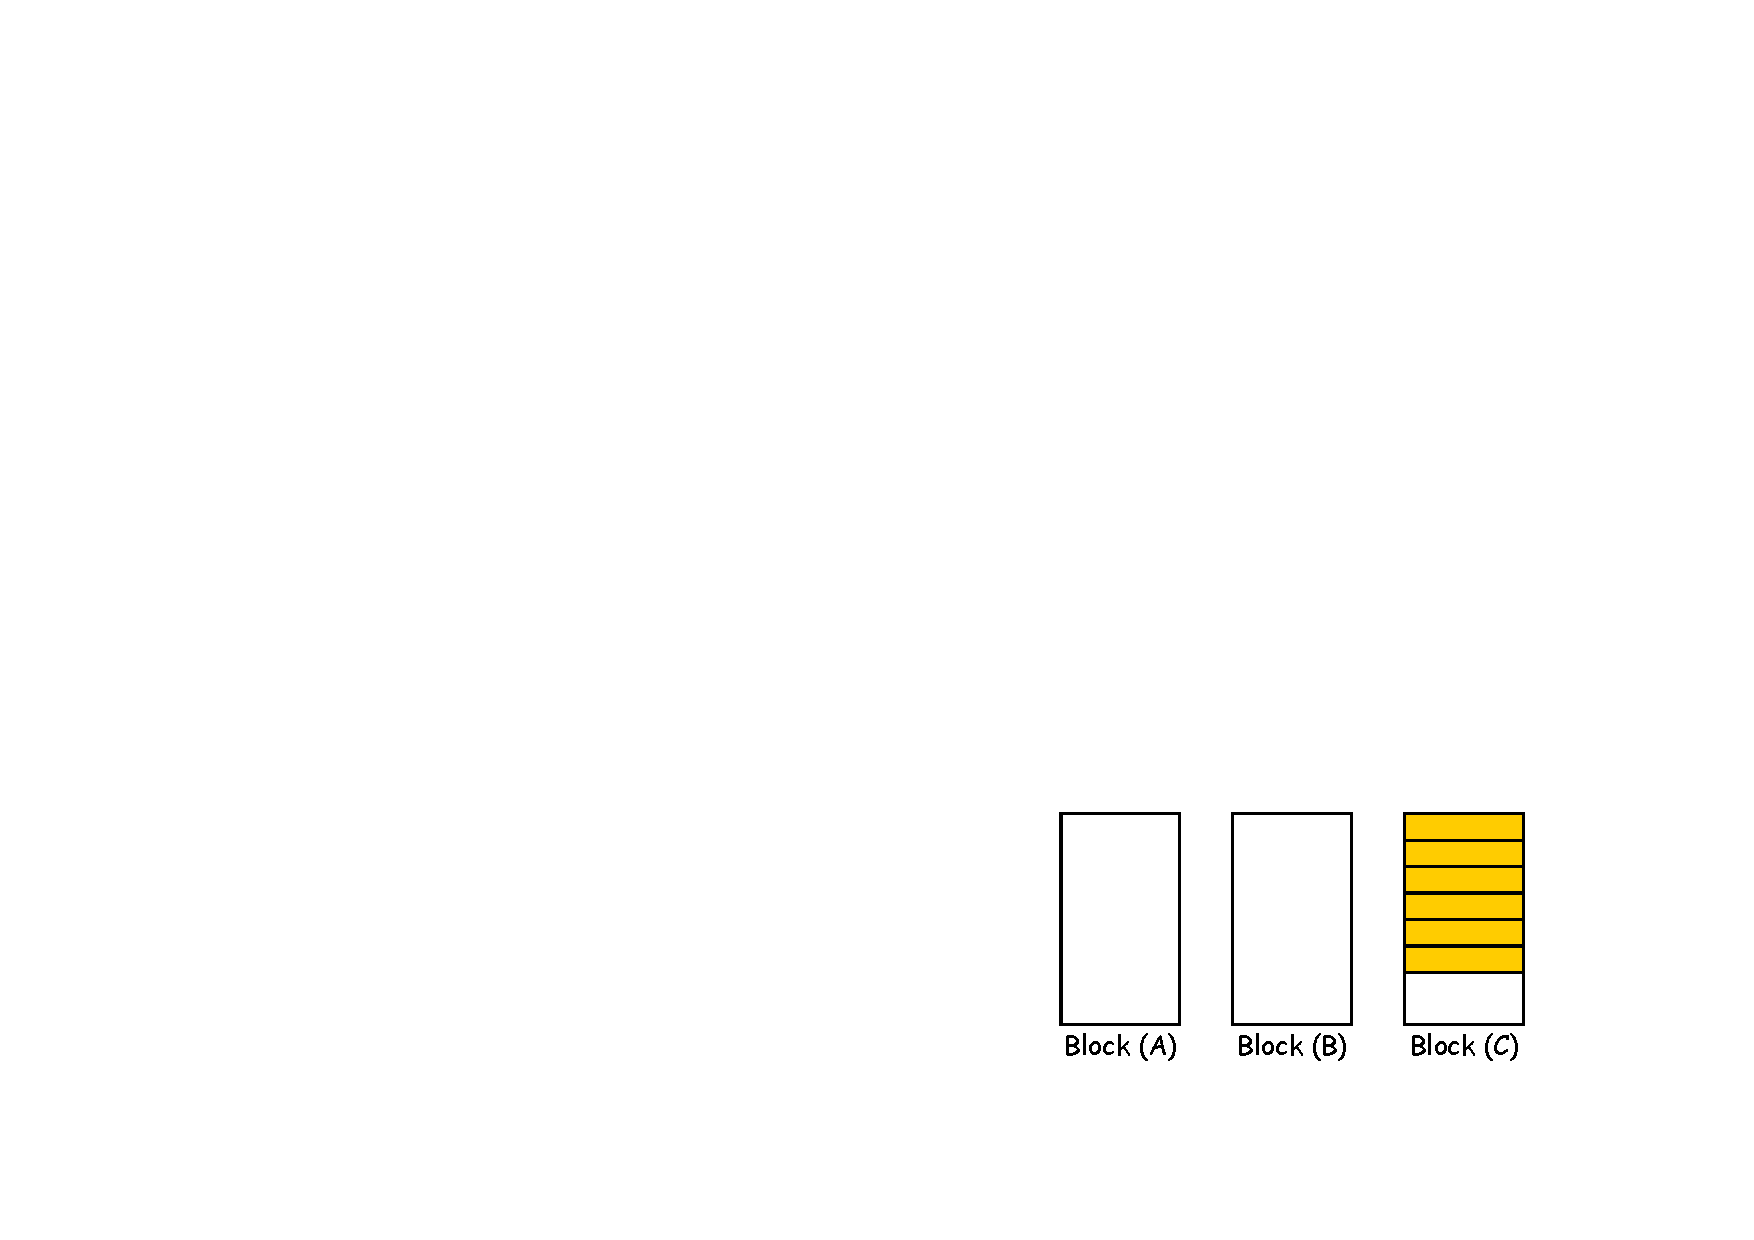
\includegraphics[width=.5\textwidth]{img/garbage-collection-5.pdf}
        \end{center}
    \end{enumerate}
\end{examplebox}

\begin{flushleft}
    \textcolor{Red2}{\faIcon{exclamation-triangle} \textbf{Problem 1: the Garbage Collection is too expensive!}}
\end{flushleft}
The Garbage Collection is \textbf{expensive}. It requires reading and rewriting of live data. Ideal garbage collection is a reclamation of a block that consists of only dead pages.

\highspace
\begin{flushleft}
    \textcolor{Green3}{\faIcon{check} \textbf{Partial solution}}
\end{flushleft}
Garbage Collection \textbf{costs depend on the amount of data blocks that must be migrated}. The \underline{\textbf{solution}} to alleviate the problem is to overprovision the device by \textbf{adding extra flash capacity} (cleaning can be delayed) and \textbf{running the garbage collection in the background} using less busy periods for the disk.

\highspace
\begin{flushleft}
    \textcolor{Red2}{\faIcon{exclamation-triangle} \textbf{Problem 2: the Ambiguity of Delete}}
\end{flushleft}
When performing background Garbage Collection, the SSD assumes to know which pages are invalid. However, most file systems do not truly delete data. For example, on Linux, the \dquotes{delete} function is \texttt{unlink()}, removing the file meta-data but not the file itself.
\begin{enumerate}
    \item File is written on SSD
    \item File is deleted
    \item The Garbage Collection executes:
    \begin{itemize}
        \item 9 pages look valid to the SSD;
        \item BUT the OS knows only 2 pages are valid.
    \end{itemize}
\end{enumerate}

\highspace
\begin{flushleft}
    \textcolor{Green3}{\faIcon{check} \textbf{Partial solution}}
\end{flushleft}
New SSD SATA command TRIM (SCSI - UNMAP). The \textbf{OS tells the SSD that specific LBAs} (page \pageref{LBA (Logical Block Address)}) \textbf{are invalid and may be garbaged by the Garbage Collection}.

\highspace
\begin{flushleft}
    \textcolor{Red2}{\faIcon{exclamation-triangle} \textbf{Problem 3: Mapping Table Size}}
\end{flushleft}
The \textbf{size of the page-level mapping table is too large}. In fact, with a 1 TB SSD with a 4-byte entry per 4 KB page, 1 GB of DRAM is needed for mapping!

\highspace
\begin{flushleft}
    \textcolor{Green3}{\faIcon{check} \textbf{Partial solution}}
\end{flushleft}
Exists some approaches to reduce the costs of mapping:
\begin{itemize}
    \item \definition{Block Mapping} (block-based mapping). Mapping at block granularity to reduce the size of a mapping table. With this technique, there is a small writing problem: the FTL must read a large amount of live data from the old block and copy it into a new one.
    \begin{examplebox}[: Block Mapping]
        The first four writes:
        \begin{multicols}{2}
            \begin{itemize}
                \item \texttt{Write(2000, a)}
                \item \texttt{Write(2001, b)}
                \item \texttt{Write(2002, c)}
                \item \texttt{Write(2003, d)}
            \end{itemize}
        \end{multicols}
        \begin{center}
            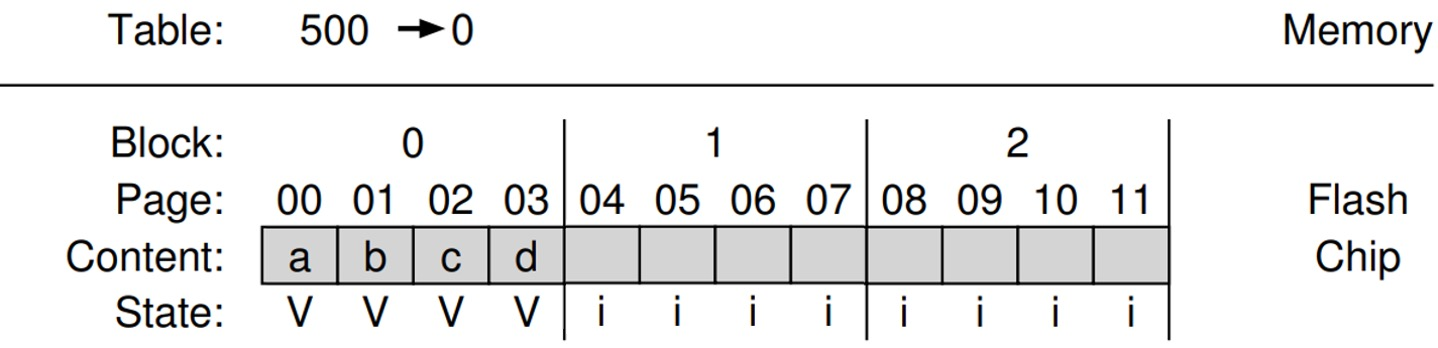
\includegraphics[width=\textwidth]{img/block-mapping-1.png}
        \end{center}

        \noindent
        And finally the last one:
        \begin{itemize}
            \item \texttt{Write(2002, c')}
        \end{itemize}
        \begin{center}
            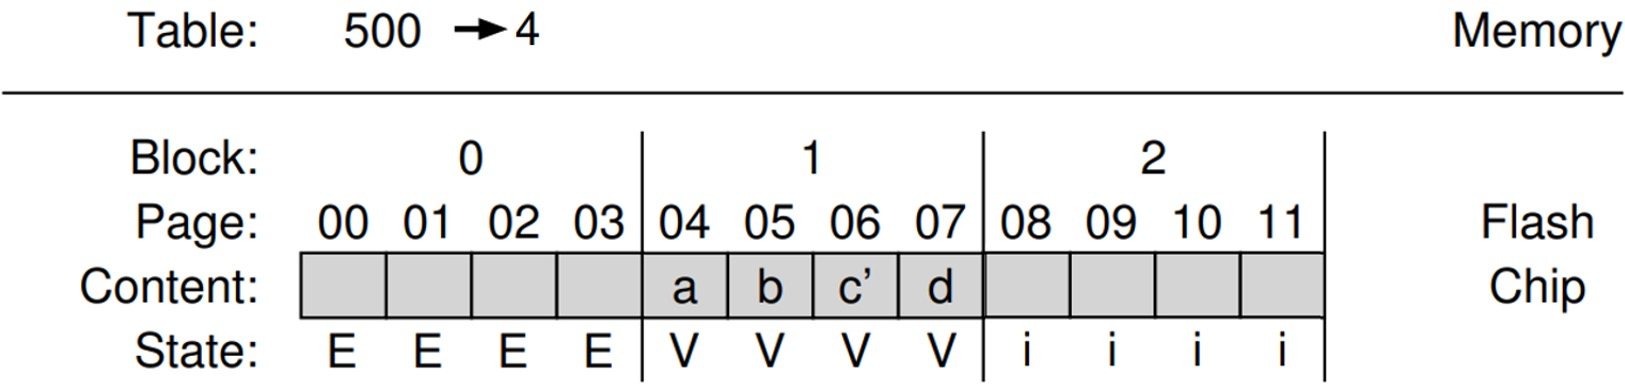
\includegraphics[width=\textwidth]{img/block-mapping-2.png}
        \end{center}
    \end{examplebox}
    
    \item \definition{Hybrid Mapping}. FTL maintains two tables: \textbf{log blocks} (page mapped) and \textbf{data blocks} (block mapped). The FTL will consult the page mapping table and block mapping table when looking for a particular logical block.
    \begin{examplebox}[: Hybrid Mapping]
        Let's suppose the following sequence:
        \begin{multicols}{2}
            \begin{itemize}
                \item \texttt{Write(1000, a)}
                \item \texttt{Write(1001, b)}
                \item \texttt{Write(1002, c)}
                \item \texttt{Write(1003, d)}
            \end{itemize}
        \end{multicols}
        \begin{center}
            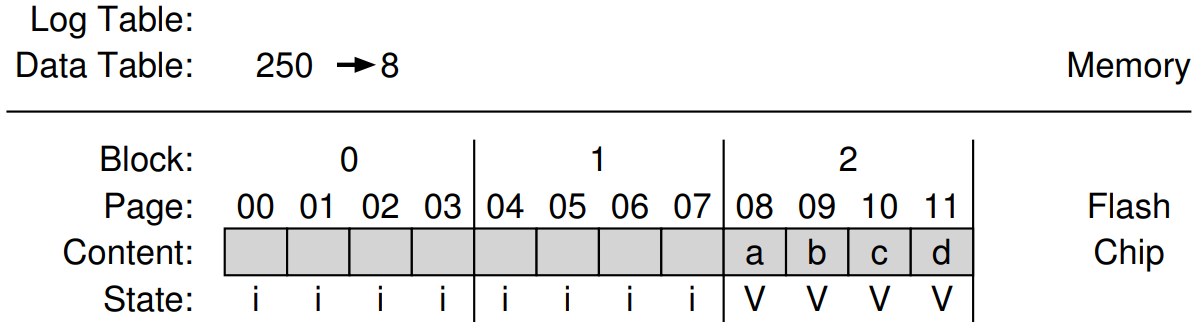
\includegraphics[width=\textwidth]{img/hybrid-mapping-1.png}
        \end{center}
        Let's update some pages:
        \begin{itemize}
            \item \texttt{Write(1000, a')}
            \item \texttt{Write(1001, b')}
            \item \texttt{Write(1002, c')}
            \item FTL updates only the page mapping information
        \end{itemize}
        \begin{center}
            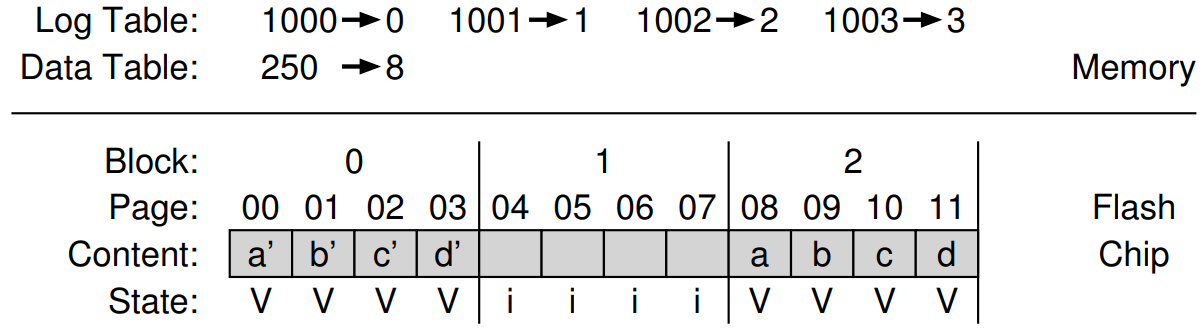
\includegraphics[width=\textwidth]{img/hybrid-mapping-2.png}
        \end{center}
        When needed, FTL can perform MERGE operations:
        \begin{center}
            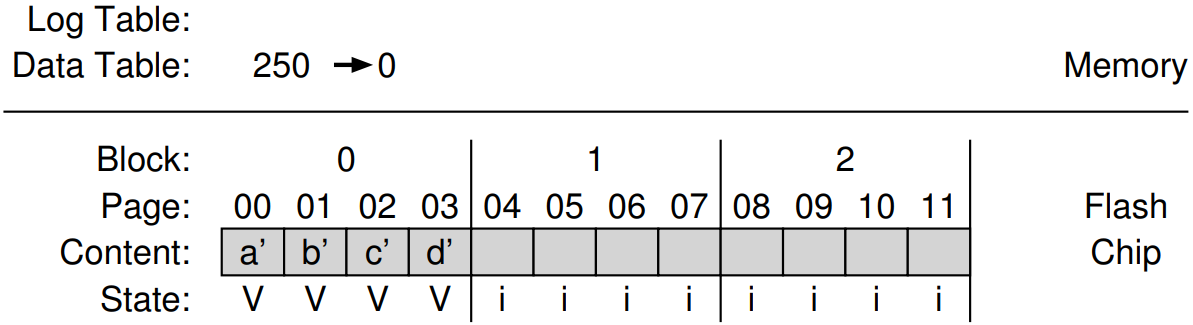
\includegraphics[width=\textwidth]{img/hybrid-mapping-3.png}
        \end{center}
    \end{examplebox}
    
    \item \definition{Page Mapping plus Caching}. The basic idea is to \textbf{cache the active part of the page-mapped FTL}. If a given workload only accesses a small set of pages, the translations of those pages will be stored in the FTL memory. It will perform well without high memory cost if the cache can contain the necessary working set. Cache miss overhead exists; we need to accept it.
\end{itemize}

\begin{flushleft}
    \textcolor{Green3}{\faIcon{check} \textbf{The importance of Wear Leveling}}
\end{flushleft}
As we have mentioned, the wear leveling is essential. The erase/write cycle is limited in Flash Memory. All blocks should wear out roughly at the same time.

\highspace
The log-structured approach and garbage collection help spread writing. However, a block may contain cold data: the FTL must periodically read all the live data from such blocks and re-write it elsewhere.
A \textbf{disadvantage} is that the wear levelling \textbf{increases the write amplification} of the SSD and consequently decreases performance. However, to \textbf{partially fix} this, a simple policy to apply is that each flash block has an \definition{Erase/Write Cycle Counter} and maintains the value of:
\begin{equation}
    \left| \mathrm{Max}\left(\text{EW cycle}\right) - \mathrm{Min}\left(\text{EW cycle}\right) \right| < e
\end{equation}

\begin{flushleft}
    \textcolor{Red2}{\textbf{HDD vs SSD}}
\end{flushleft}
Exists two metrics:
\begin{itemize}
    \item \definition{Unrecoverable Bit Error Ratio (UBER)}. A metric for the rate of occurrence of data errors, equal to the \textbf{number of data errors per bits read}.
    
    \item \definition{Endurance rating: Terabytes Written (TBW)}. It is the total amount of data that can be written into an SSD before it is likely to fail. \textbf{The number of terabytes that may be written to the SSD while still meeting the requirements}.
\end{itemize}
\begin{figure}[!htp]
    \centering
    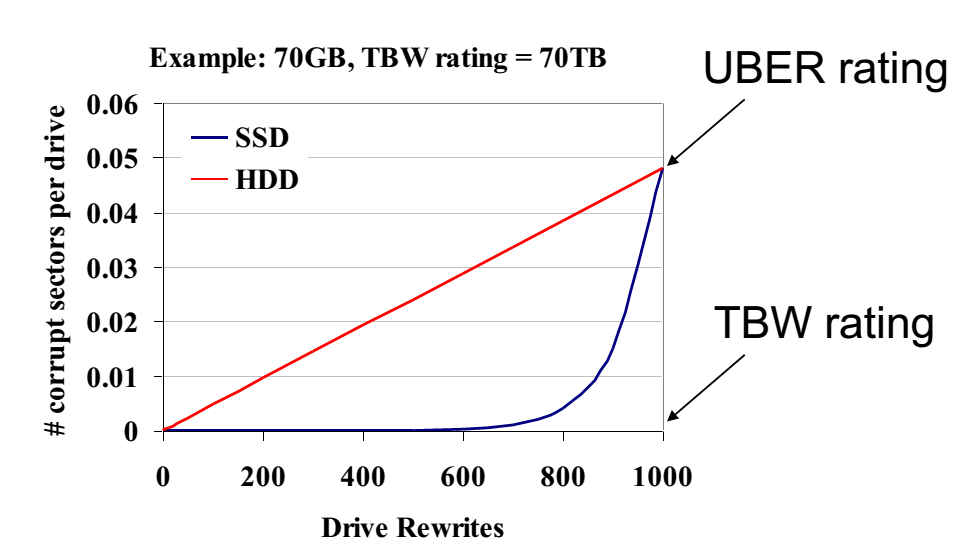
\includegraphics[width=.7\textwidth]{img/hdd-vs-ssd.png}
\end{figure}

\newpage

\paragraph{RAID}\label{paragraph: RAID}

\definition{RAID (Redundant Array of Independent Disks)} is a \textbf{data storage virtualization technology}\footnote{I/O virtualization: data are distributed transparently over the disks, then no action is required of the users.} that \textbf{combines multiple physical disk drive components into one or more logical units for the purposes of data redundancy}, \textbf{performance improvement}, or both. This contrasts the previous concept of highly reliable mainframe disk drives, which were referred to as  \definition{Single Large Expensive Disks (SLED)}, also called \definition{Just a Bunch of Disks (JBOD)} method where each disk is a separate device with a different mount point.

\highspace
The data are striped across several disks accessed in parallel:
\begin{itemize}
    \item \textbf{High data transfer rate}: large data accesses (heavy I/O operations).
    \item \textbf{High I/O rate}: small but frequent data accesses (light I/O operations).
    \item \textbf{Load Balancing} across the disks.
\end{itemize}
Two techniques exist to guarantee these features: \textbf{data striping} (improve performance) and \textbf{redundancy} (improve reliability).

\highspace
\definition{Data Striping} is the technique of \textbf{segmenting logically sequential data}, such as a file, so that \textbf{consecutive segments are stored on different physical storage devices}. A small quantity of terminology:
\begin{itemize}
    \item \definition{Striping}: \textbf{data are written sequentially} (a vector, a file, a table, etc) in units (stripe units such as bit, byte, and blocks) \textbf{on multiple disks} according to a cyclic algorithm (round robin).

    \item \definition{Stripe unit}: the \textbf{dimension of the data unit written on a single disk}.

    \item \definition{Stripe width}: number of \textbf{disks considered by the striping algorithm}:
    \begin{enumerate}
        \item \textbf{Multiple independent I/O requests} will be executed in parallel by several disks, decreasing the disks' queue length (and time).

        \item Multiple disks will execute \textbf{single Multiple-Block I/O requests} in parallel, increasing the transfer rate of a single request.
    \end{enumerate}
\end{itemize}

\highspace
The \textbf{redundancy technique is introduced because} the more physical disks in the array, the more significant the size and performance gains, but the \textbf{larger the probability of failure of a disk}.

In fact, the \emph{probability of a failure} (assuming independent failures) in an array of 100 disks is 100 higher than the probability of a failure of a single disk! For \textcolor{Green4}{\textbf{example}}, if a disk has a \definition{Mean Time To Failure (MTTF)} of 200.000 hours (23 years), an array of 100 disks will show an MTTF of 2000 hours (3 months).

\highspace
The \definition{Redundancy} is the \textbf{technique of data duplication or error correcting codes} (stored on disks different from the ones with the data) \textbf{that are computed to tolerate loss due to disk failures}. Since write operations must also update the redundant information, their \textbf{performance is worse than traditional writing}.

\highspace
Data is distributed across the drives in one of several ways, referred to as \definition{RAID levels}, depending on the required level of redundancy and performance. The different schemes, or data distribution layouts, are named by the word \emph{RAID} followed by a number, for example RAID 0 or RAID 1. Each scheme, or RAID level, provides a different balance among the key goals: reliability, availability, performance, and capacity. The RAID levels are:
\begin{itemize}
    \item \texttt{RAID 0} striping only
    \item \texttt{RAID 1} mirroring only
    \begin{itemize}
        \item \texttt{RAID 0+1} nested levels
        \item \texttt{RAID 1+0} nested levels
    \end{itemize}
    \item \texttt{RAID 2} bit interleaving (not used)
    \item \texttt{RAID 3} byte interleaving - redundancy (parity disk)
    \item \texttt{RAID 4} block interleaving - redundancy (parity disk)
    \item \texttt{RAID 5} block interleaving - redundancy (parity block distributed)
    \item \texttt{RAID 6} greater redundancy (2 failed disks are tolerated)
\end{itemize}
Note: these notes do \underline{not} study the levels \texttt{RAID 2} and \texttt{RAID 3}.

\begin{table}[!htp]
    \centering
    \begin{tabular}{@{} l l @{}}
        \toprule
        \textbf{Topic} & \textbf{Page} \\
        \midrule
        \texttt{RAID 0} & \hyperlink{RAID 0}{\hypergetpageref{RAID 0}} \\
        \texttt{RAID 1} & \hyperlink{RAID 1}{\hypergetpageref{RAID 1}} \\
        \texttt{RAID 0 + 1} & \hyperlink{RAID 0 + 1}{\hypergetpageref{RAID 0 + 1}} \\
        \texttt{RAID 1 + 0} & \hyperlink{RAID 1 + 0}{\hypergetpageref{RAID 1 + 0}} \\
        \texttt{RAID 4} & \hyperlink{RAID 4}{\hypergetpageref{RAID 4}} \\
        \texttt{RAID 5} & \hyperlink{RAID 5}{\hypergetpageref{RAID 5}} \\
        \texttt{RAID 6} & \hyperlink{RAID 6}{\hypergetpageref{RAID 6}} \\
        Comparison and characteristics of RAID levels & \hyperlink{Comparison and characteristics of RAID levels}{\hypergetpageref{Comparison and characteristics of RAID levels}} \\
        \bottomrule
    \end{tabular}
    \caption{RAID - Table of Contents.}
\end{table}

\newpage

\begin{center}\label{RAID 0}
    \large
    \hypertarget{RAID 0}{\textcolor{Red2}{\textbf{RAID 0}}}
\end{center}

\noindent
In RAID 0, the data are \textbf{written on a single logical disk and split into several blocks distributed across the disks} according to a striping algorithm.

\begin{flushleft}
    \textcolor{Green3}{\faIcon{question-circle} \textbf{When is it used?}}
\end{flushleft}
It is used where \textbf{performance} and \textbf{capacity} are the primary concerns. These mean that a minimum of two drives is required.

\highspace
\begin{flushleft}
    \textcolor{Green3}{\faIcon{check} \textbf{Advantages}}
\end{flushleft}
\begin{itemize}
    \item \textbf{Lower cost} because it does not employ redundancy (no error-correcting codes are computed and stored).
    \item \textbf{Best write performance} (it does not need to update redundant data and is parallelized).
\end{itemize}

\highspace
\begin{flushleft}
    \textcolor{Red2}{\faIcon{exclamation-triangle} \textbf{Disadvantages}}
\end{flushleft}
\textbf{Single disk failure} will result in data loss.

\highspace
\begin{flushleft}
    \textcolor{Green3}{\faIcon{tools} \textbf{How does it work?}}
\end{flushleft}
The key idea is to present an \textbf{array of disks as a single large disk} and maximize parallelism by striping data across all $N$ disks.

\highspace
Now, we will give some metrics to understand how it is possible to \textbf{calculate access to a specific data block} and compare the \textbf{performance} of different RAID technologies.

\highspace
To \textbf{access to a specific data blocks}, the formulas are:
\begin{equation}
    \begin{array}{rcl}
        \texttt{Disk}    &=& \texttt{logical\_block\_number} \: \% \: \texttt{number\_of\_disks} \\ [.5em]
        \texttt{Offset}  &=& \dfrac{\texttt{logical\_block\_number}}{\texttt{number\_of\_disks}}
    \end{array}
\end{equation}
For example, given the following schema:
\begin{figure}[!htp]
    \centering
    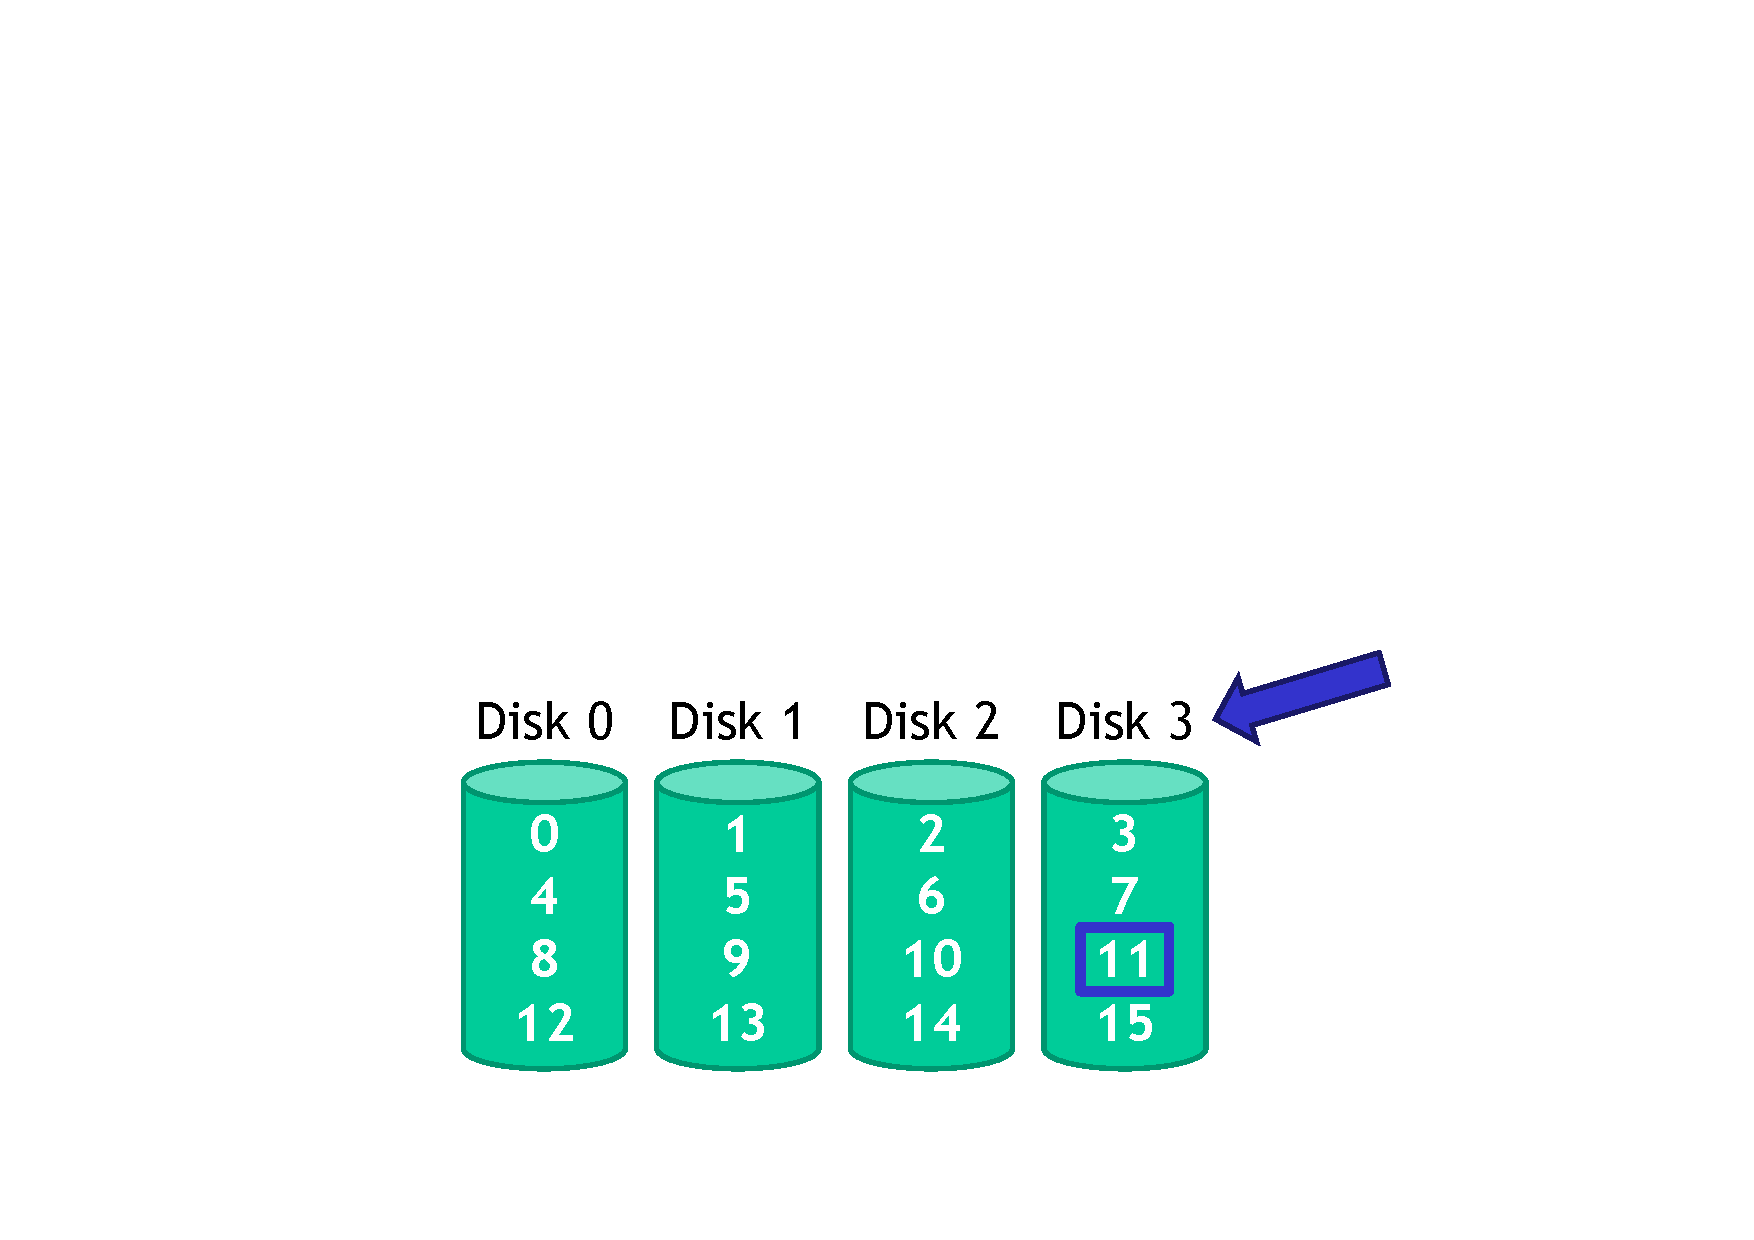
\includegraphics[width=.5\textwidth]{img/raid-1.pdf}
\end{figure}

\noindent
If it is requested, the logical block is 11, and the disks are 4:
\begin{equation*}
    \begin{array}{rcl}
        \texttt{Disk}    &=& 11 \% 4 = 3 \\ [.5em]
        \texttt{Offset}  &=& 11 \div 4 = 2.75 \approx 3, \text{ then physical block 2 starting from 0}
    \end{array}
\end{equation*}
Note that the \textbf{chunk size is critical} because it impacts disk array performance. With \textbf{smaller chunks}, there is \textbf{greater parallelism} than with \textbf{big chunks}, which have \textbf{reduced seek times}. The typical arrays use 64 KB chunks.

\highspace
To measure RAID \textbf{performance}, we focus on sequential and random workloads. Assume disks in the array have sequential transfer rate S, and the info about the disk is:
\begin{itemize}
    \item Average seek time: 7 ms
    \item Average rotational delay: 3 ms
    \item Transfer rate: 50 MB/s
\end{itemize}
For a single large transfer (10 MB):
\begin{equation*}
    \begin{array}{rcl}
        S &=& \dfrac{\texttt{transfer\_size}}{\texttt{time\_to\_access}} \\ [1.2em]
        S &=& 10 \text{ MB} \div \left(7 \text{ ms} + 3 \text{ ms} + 10 \text{ MB} \div 50 \text{ MB/s}\right) = 47.62 \text{ MB/s}
    \end{array}
\end{equation*}
If the disks in the array have a random transfer rate R, and for a set of small files (10 KB):
\begin{equation*}
    \begin{array}{rcl}
        R &=& \dfrac{\texttt{transfer\_size}}{\texttt{time\_to\_access}} \\ [1.2em]
        R &=& 10 \text{ KB} \div \left(7 \text{ ms} + 3 \text{ ms} + 10 \text{ KB} \div 50 \text{ MB/s}\right) = 0.98 \text{ MB/s}
    \end{array}
\end{equation*}

\highspace
\begin{flushleft}
    \textcolor{Green3}{\faIcon{chart-bar} \textbf{Analysis}}
\end{flushleft}
\begin{itemize}
    \item \textbf{Capacity}: $N$, where $N$ is the number of disks. Then, everything can be filled with data.

    \item \textbf{Reliability}: non-existent. If any drive fails, data is permanently lost. Then, the Mean Time To Failure (MTTF) equals the \definition{Mean Time To Data Loss (MTTDL)}:
    \begin{equation*}
        \texttt{MTTF} = \texttt{MTTDL}
    \end{equation*}

    \item \textbf{Sequential read and write}: $N \times S$

    \item \textbf{Random read and write}: $N \times R$
\end{itemize}
Where $N$ is the number of disks, $S$ the sequential transfer rate and $R$ the random transfer rate.

\newpage

\begin{center}\label{RAID 1}
    \large
    \hypertarget{RAID 1}{\textcolor{Red2}{\textbf{RAID 1}}}
\end{center}

\noindent
Although RAID 0 offers high performance, it has zero error recovery. For this reason, RAID 1 makes \textbf{two copies of all data} (again, a minimum of 2 disk drives are required).

\begin{flushleft}
    \textcolor{Green3}{\faIcon{question-circle} \textbf{When is it used?}}
\end{flushleft}
It is used when \textbf{zero error recovery is not allowed}.

\highspace
\begin{flushleft}
    \textcolor{Green3}{\faIcon{check} \textbf{Advantages}}
\end{flushleft}
\begin{itemize}
    \item \textbf{High reliability}. When a disk fails, the \emph{second copy is used}.
    \item \textbf{Read of a data}. It can be \emph{retrieved} from the \emph{disk with shorter queueing, seek, and latency delays}.
    \item \textbf{Fast writes} (no error correcting code should be computed). But \emph{still slower than standard disks} (due to duplication).
\end{itemize}

\highspace
\begin{flushleft}
    \textcolor{Red2}{\faIcon{exclamation-triangle} \textbf{Disadvantages}}
\end{flushleft}
\begin{itemize}
    \item \textbf{High costs} because only 50\% of the capacity is used.
\end{itemize}

\highspace
\begin{flushleft}
    \textcolor{Green3}{\faIcon{tools} \textbf{How does it work?}}
\end{flushleft}
In principle, a RAID 1 can mirror the content over more than one disk. This feature gives resiliency to errors even if more than one disk breaks. Also, it allows a \textbf{voting mechanism to identify errors not reported by the disk controller}. Unfortunately, this is \textbf{never used in practice because the overhead and costs are \underline{too high}}.

\highspace
However, disks could be coupled if several disks are available (always in an \underline{even} number). Nevertheless, the total capacity is halved, and each disk has a mirror. Then, the question is simple: \emph{How do we organize this architecture?} The answer is the nested RAIDs: \texttt{RAID 0 + 1} and \texttt{RAID 1 + 0}.

\highspace
We define the \texttt{RAID x + y} (or \texttt{RAID xy}) as:
\begin{itemize}
    \item $n \times m$ disks in total
    \item $m$ groups of $n$ disks
    \item Apply \texttt{RAID x} to each group of $n$ disks
    \item Apply \texttt{RAID y} considering the $m$ groups as single disks
\end{itemize}
\newpage
\begin{figure}[!htp]
    \centering
    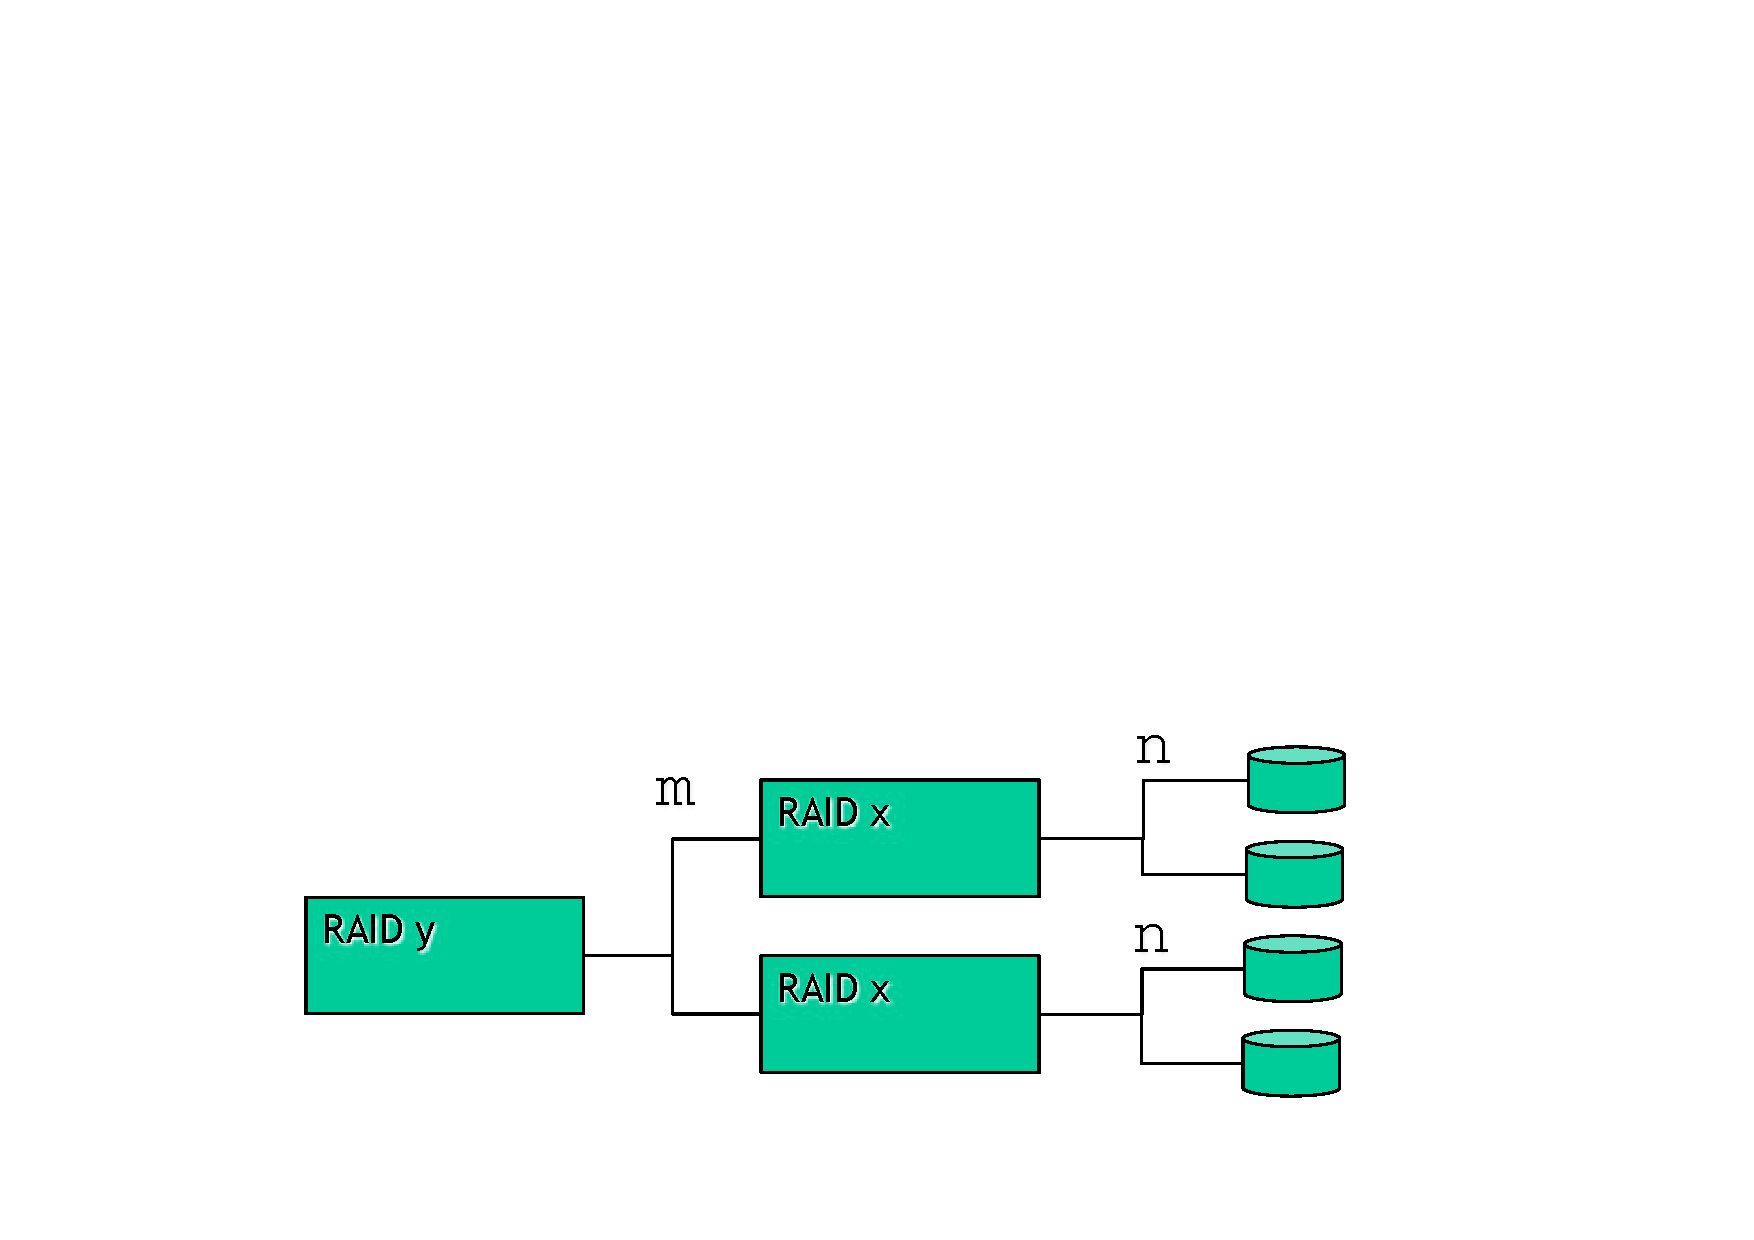
\includegraphics[width=.6\textwidth]{img/raid-2.pdf}
    \caption{\texttt{RAID x + y} general architecture.}
\end{figure}

\label{RAID 0 + 1}\noindent
The \hypertarget{RAID 0 + 1}{\texttt{\textbf{RAID 0 + 1}}} is a \textbf{group of striped disks (RAID 0) that are then mirrored (RAID 1)}. So:
\begin{enumerate}
    \item The mirroring first (RAID 1)
    \item Then the striping (RAID 0)
\end{enumerate}
There are necessary almost four drives. Note that after the first failure, the model becomes a RAID 0.
\begin{figure}[!htp]
    \centering
    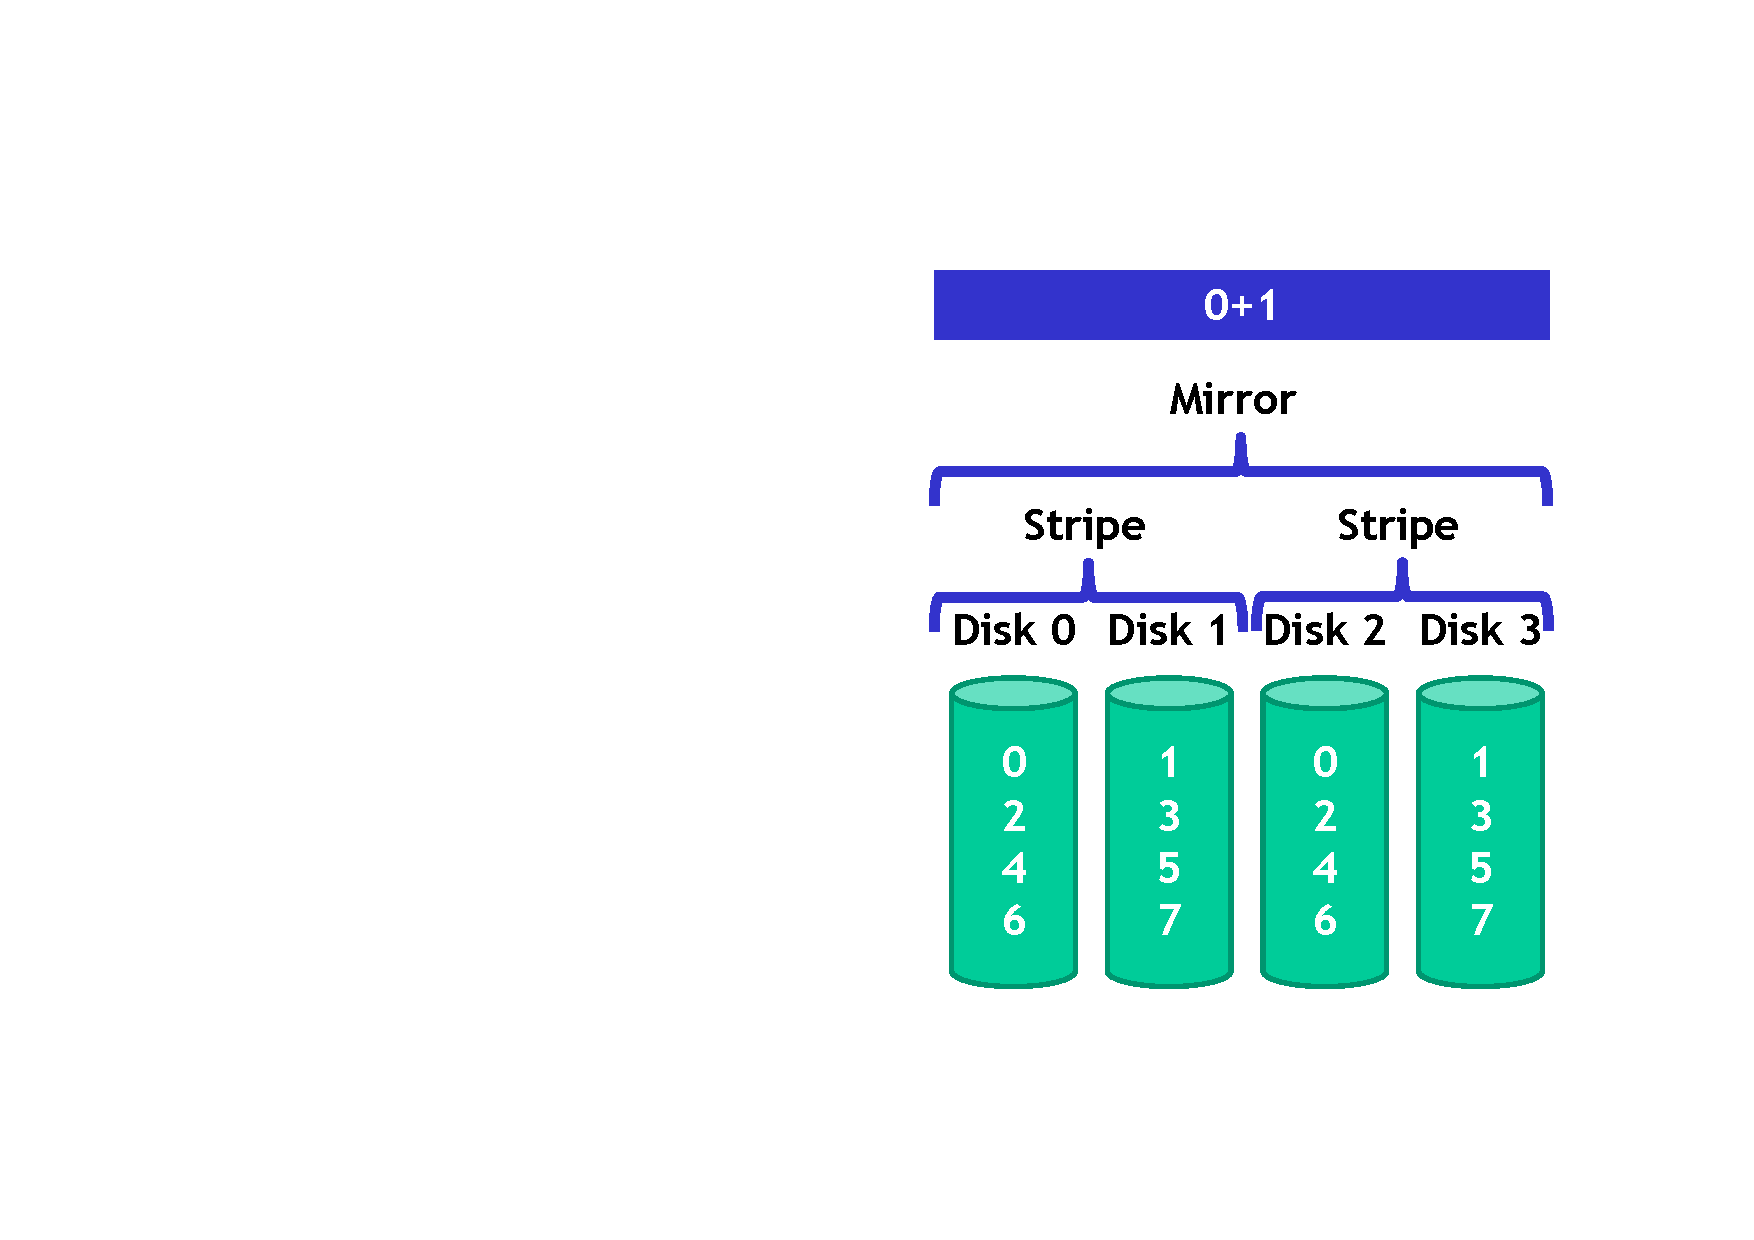
\includegraphics[width=.5\textwidth]{img/raid-3.pdf}
\end{figure}

\label{RAID 1 + 0}\highspace
The \hypertarget{RAID 1 + 0}{\texttt{\textbf{RAID 1 + 0}}} is a \textbf{group of mirrored disks (RAID 1) that are then striped (RAID 0)}. So: 
\begin{enumerate}
    \item The striping first (RAID 0)
    \item Then the mirroring (RAID 1)
\end{enumerate}
There are necessary almost four drives. Usually, it is used in databases with very high workloads (fast writes).
\newpage
\begin{figure}[!htp]
    \centering
    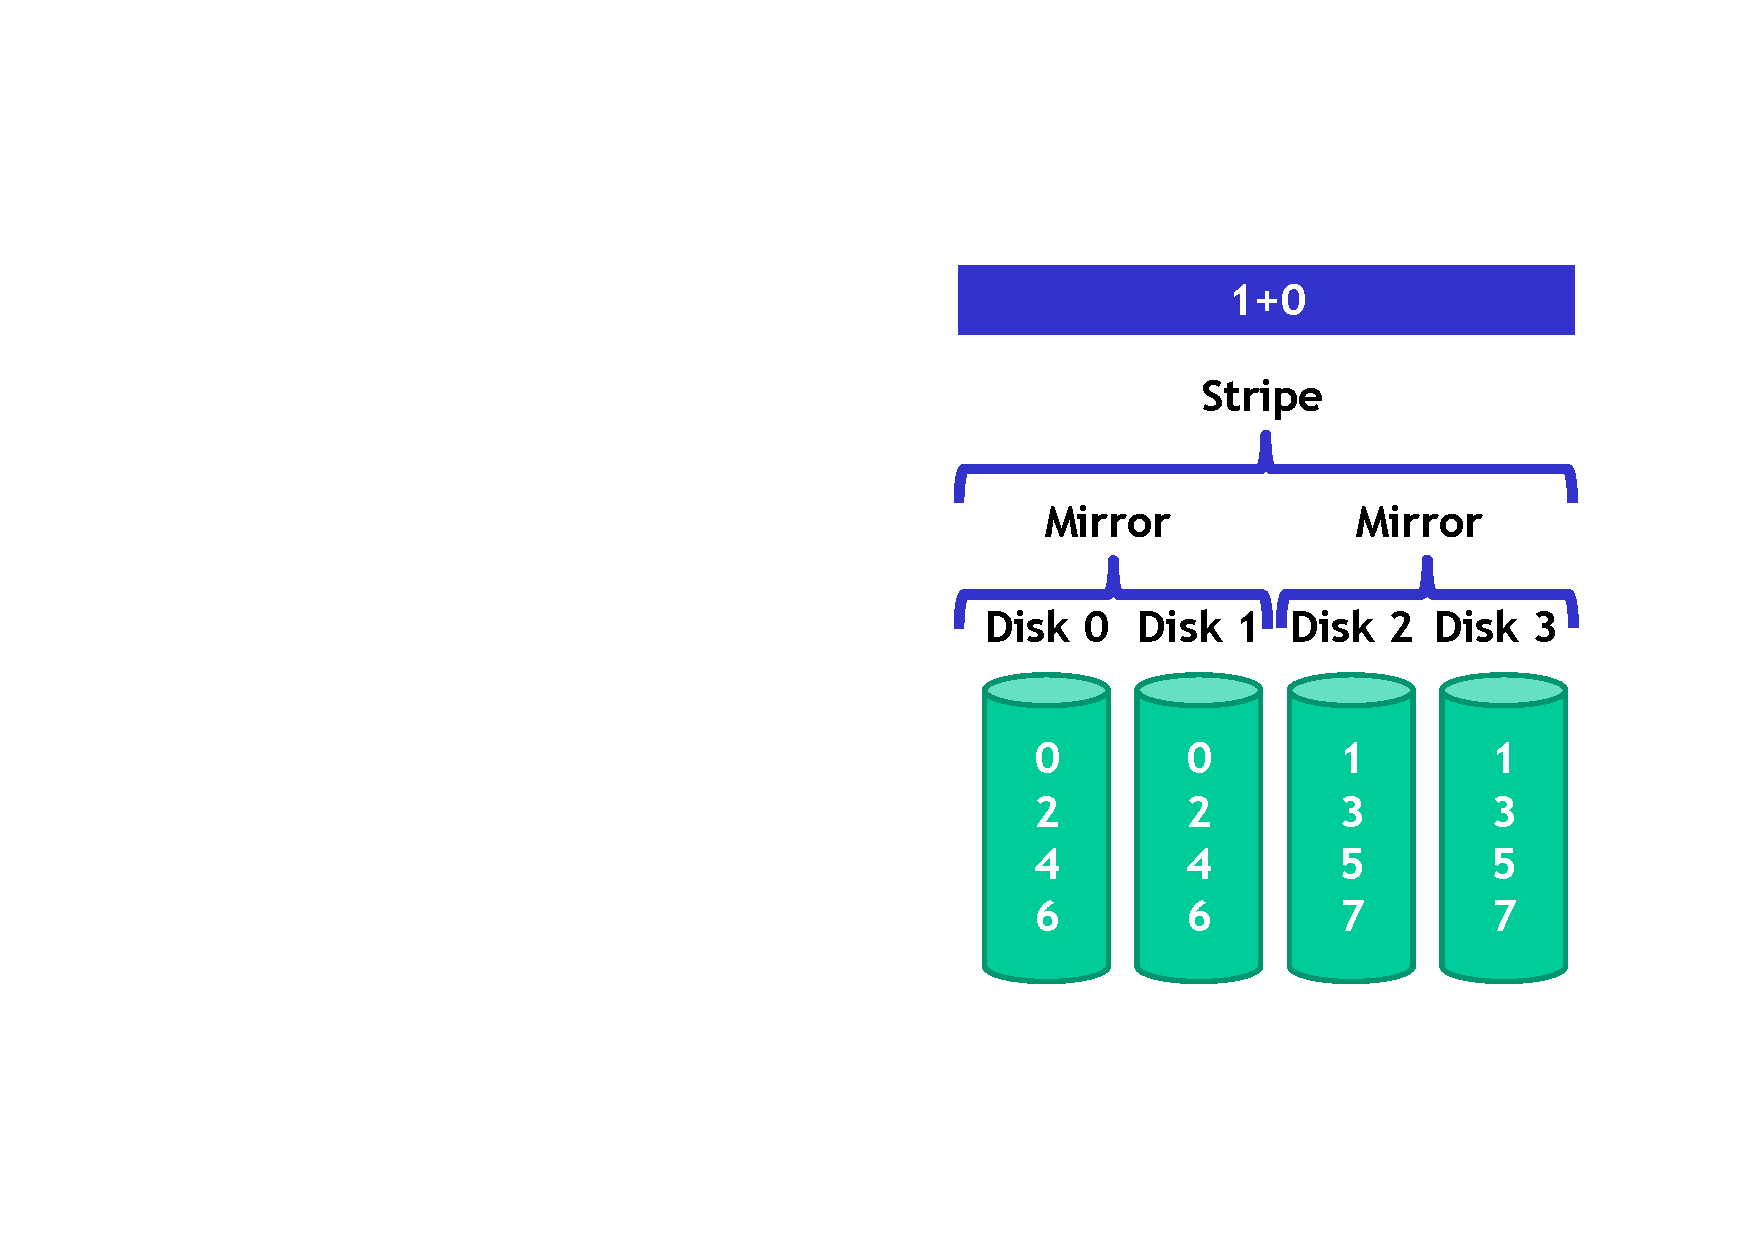
\includegraphics[width=.5\textwidth]{img/raid-4.pdf}
\end{figure}

\highspace
\begin{flushleft}
    \textcolor{Green3}{\faIcon{not-equal} \textbf{Differences between RAID 01 and RAID 10}}
\end{flushleft}
Look at the following architectures:
\begin{figure}[!htp]
    \centering
    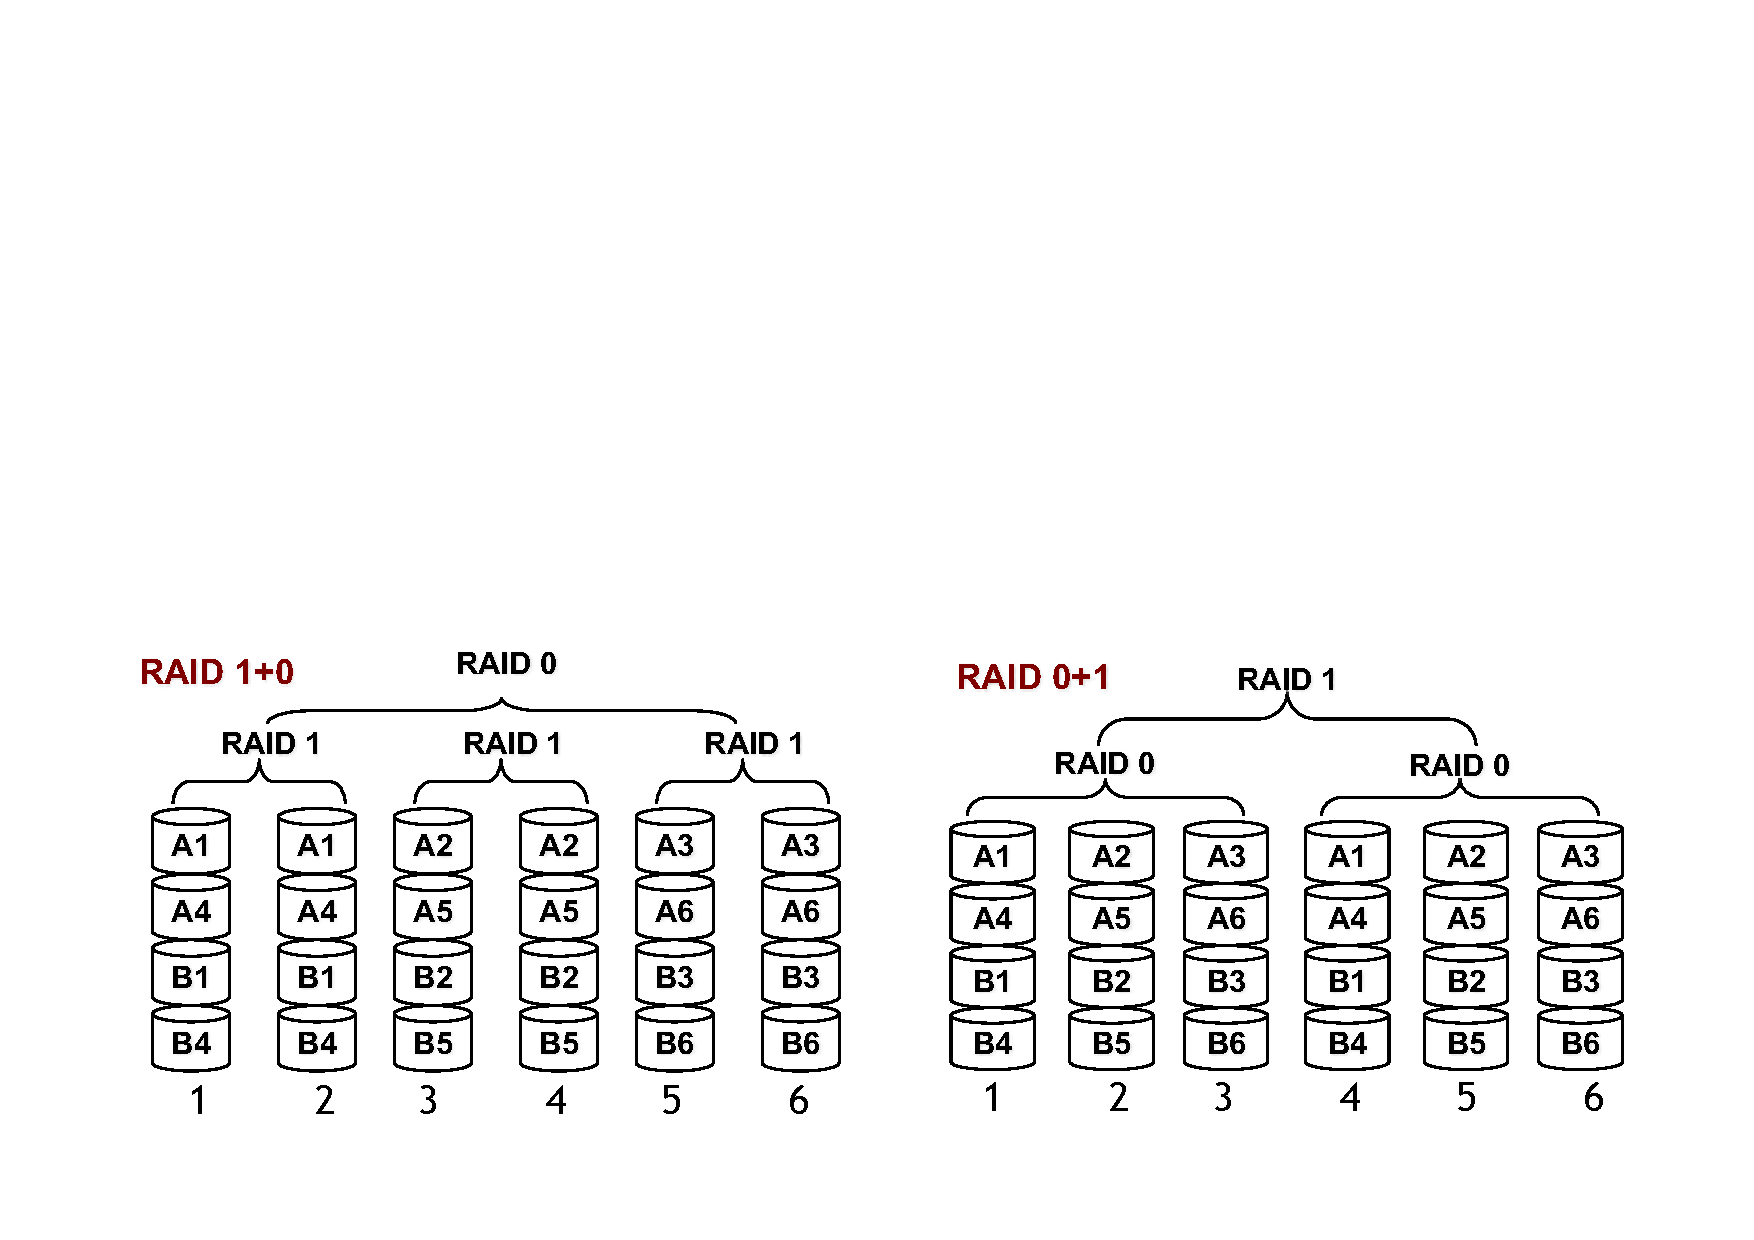
\includegraphics[width=\textwidth]{img/raid-5.pdf}
\end{figure}

\noindent
What we can say is:
\begin{itemize}
    \item The performance of RAID 01 and RAID 10 are the same.
    \item The \textbf{main difference is the fault tolerance}\footnote{Fault tolerance is the ability of a system to maintain proper operation despite failures or faults in or more of its components.}!
\end{itemize}
On most implementations of RAID controllers, \textbf{RAID 01 fault tolerance is less}. Since we have only two groups of RAID 0, if two drives (one in each group) fail, the entire RAID 01 will fail. Looking at the architecture above, if Disk 1 and 4 fail, both groups will be down. So, the whole RAID 01 will fail.

On the contrary, RAID 10 since there are many groups (as the individual group is only two disks), even if three disks fail (one in each group), the RAID 10 is still functional. Looking at the architecture above, even if Disk 1, 3, and 5 fail, the RAID 10 will still be functional.
\begin{equation*}
    \text{Fault Tolerance: } \texttt{RAID 01} \ggg \texttt{RAID 10}
\end{equation*}
So, given a choice between RAID 10 and RAID 01, it should be better to choose RAID 10 to have more fault tolerance.

\highspace
\begin{flushleft}
    \textcolor{Green3}{\faIcon{chart-bar} \textbf{Analysis}}
\end{flushleft}
\begin{itemize}
    \item \textbf{Capacity}: $N \div 2$, where $N$ is the number of disks. Then, two copies of all data, thus half capacity.

    \item \textbf{Reliability}: $1$ drive can fail, sometimes more! In an optimistic scenario, $N \div 2$ drives can fail without data loss.

    \item \textbf{Sequential write}: $\left(N \div 2\right) \times S$; two copies of all data, thus half throughput.

    \item \textbf{Sequential read}: $\left(N \div 2\right) \times S$; half of the read blocks are wasted, thus halving throughput.

    \item \textbf{Random read}: $N \times R$; it is the best scenario for RAID 1 because the read can be parallelized across all disks.

    \item \textbf{Random write}: $\left(N \div 2\right) \times R$; two copies of all data, thus half throughput.
\end{itemize}
Where $N$ is the number of disks, $S$ is the sequential transfer rate, and $R$ is the random transfer rate.

\highspace
It is essential to observe RAID 1. There is a notorious \textbf{problem} called the \definition{Consistent Update Problem}.

Mirrored writes \underline{should be atomic}. Then, all copies are written, or none are written. Unfortunately, this is very \textbf{difficult to guarantee} sometimes, for example, in a power failure scenario. To \textbf{solve} this problem, many RAID controllers include a \definition{write-ahead log}, a \textbf{battery backend}, and \textbf{non-volatile storage of pending writes}. With this system, a \textbf{recovery procedure ensures the recovery of the out-of-sync mirrored copies}.

\newpage

\begin{center}\label{RAID 4}
    \large
    \hypertarget{RAID 4}{\textcolor{Red2}{\textbf{RAID 4}}}
\end{center}

\noindent
RAID 4 consists of \textbf{block-level striping with a dedicated parity disk}.

\begin{flushleft}
    \textcolor{Green3}{\faIcon{question-circle} \textbf{When is it used?}}
\end{flushleft}
RAID 1 offers highly reliable data storage, but it uses half the space of the array capacity. To achieve the \textbf{same level of reliability without wasting capacity}, it is possible to use RAID 4, which uses \textbf{information coding techniques to build lightweight error recovery mechanisms}.

\highspace
\begin{flushleft}
    \textcolor{Green3}{\faIcon{check} \textbf{Advantages}}
\end{flushleft}
\begin{itemize}
    \item \textbf{Good performance} of random reads.
\end{itemize}

\highspace
\begin{flushleft}
    \textcolor{Red2}{\faIcon{thumbs-down} \textbf{Disadvantages}}
\end{flushleft}
\begin{itemize}
    \item \textbf{Random Write performance is terrible} due to being \emph{bottlenecked} by the parity drive.
\end{itemize}

\highspace
\begin{flushleft}
    \textcolor{Green3}{\faIcon{tools} \textbf{How does it work?}}
\end{flushleft}
Disk $N$ only stores parity information for the other $N-1$ disks. The parity is calculated using the \texttt{XOR} operation\footnote{\dquotes{A or B, but not A and B}}.

\begin{figure}[!htp]
    \centering
    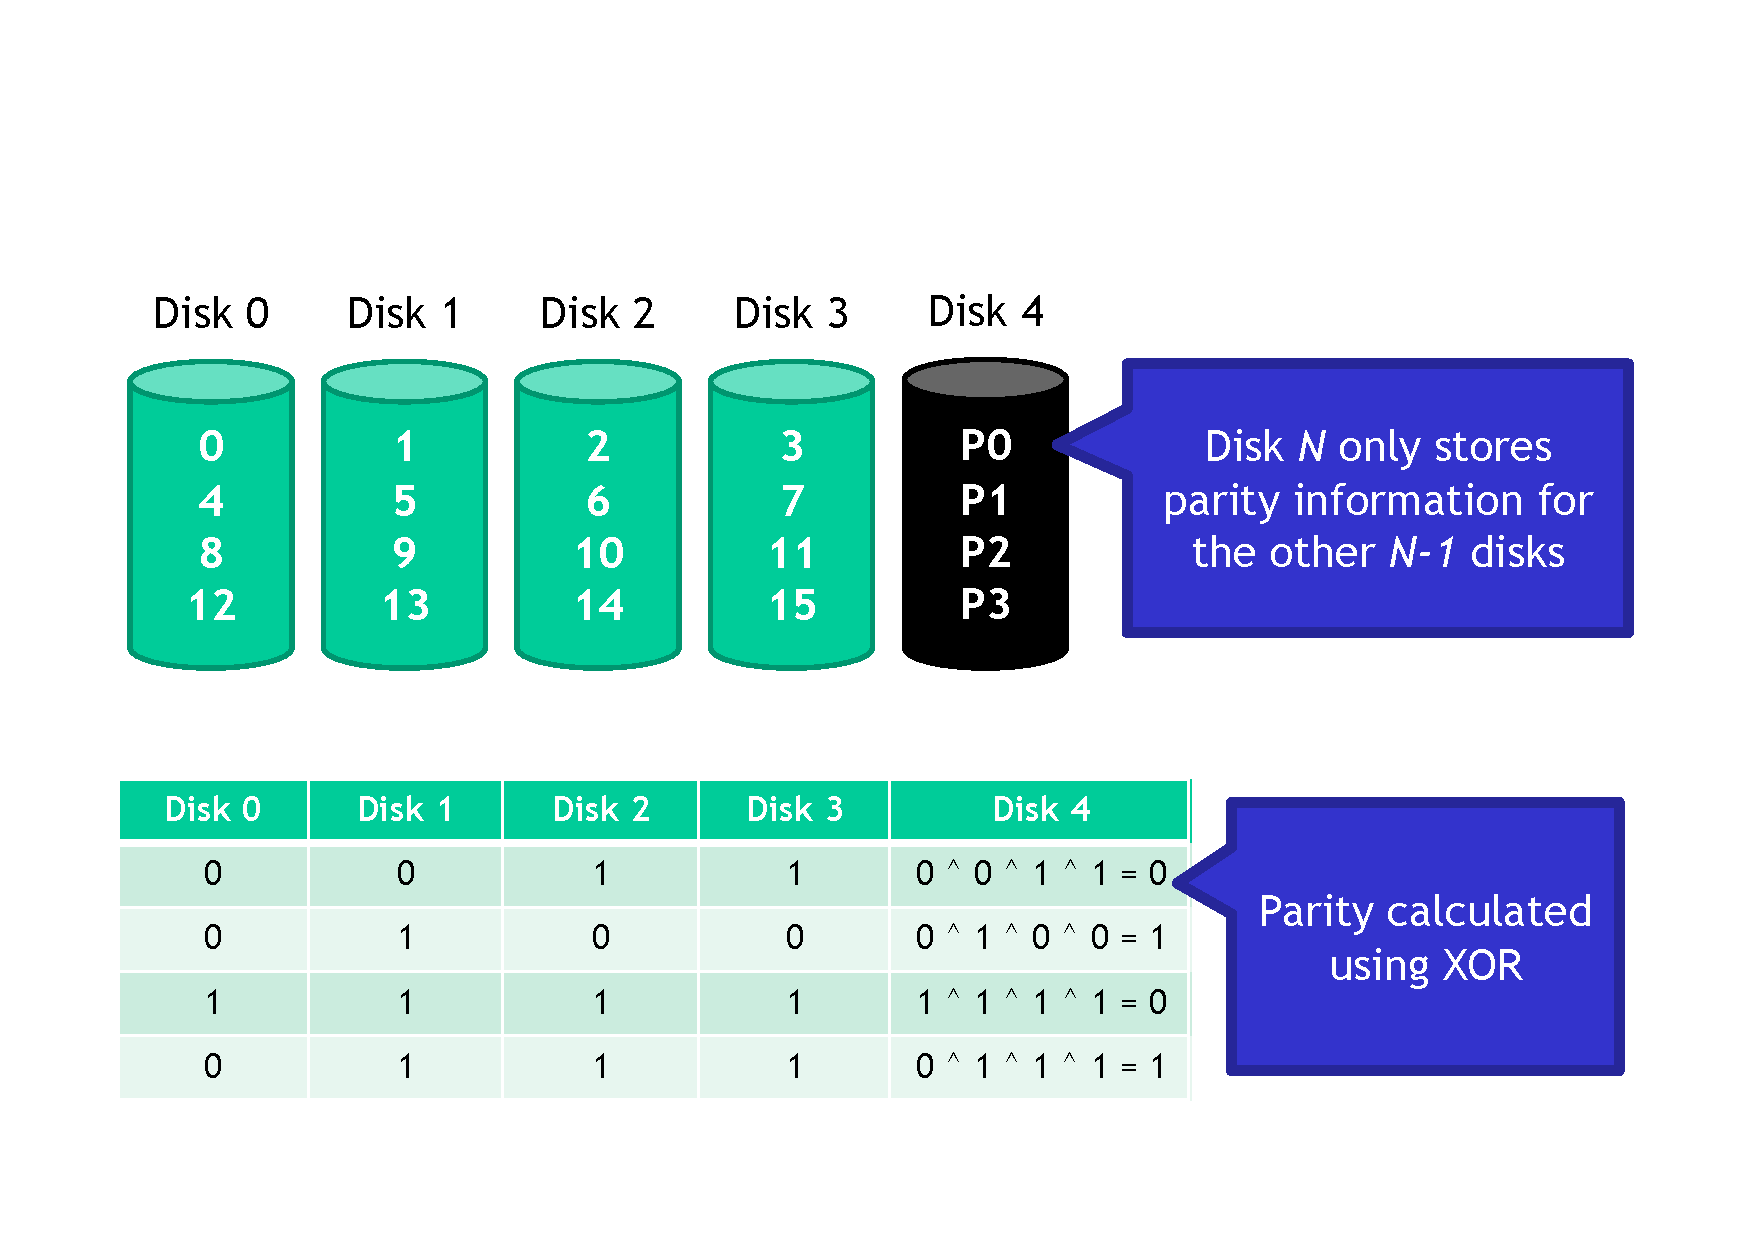
\includegraphics[width=\textwidth]{img/raid-6.pdf}
    \caption{RAID 4 - \emph{How does it work?}}
\end{figure}

\noindent
The \textbf{\underline{serial}} or \textbf{\underline{random read}} is not a problem in RAID 4 because there is a \textbf{parallelization across all non-parity blocks} in the stripe despite a tiny performance reduction due to the parity disk.

\newpage

\noindent
During the parity writing, the blocks are updated. The \textbf{\underline{random write}} performance is affected by the approach used:
\begin{itemize}
    \item \definition{Additive parity} (as known as reconstruct-writes):\index{reconstruct-writes}
    \begin{enumerate}
        \item Read all other blocks in a stripe in parallel;
        \item \texttt{XOR} those with the new block to form a new parity block;
        \item Write the new data block and new parity block to disks.
    \end{enumerate}
    \begin{figure}[!htp]
        \centering
        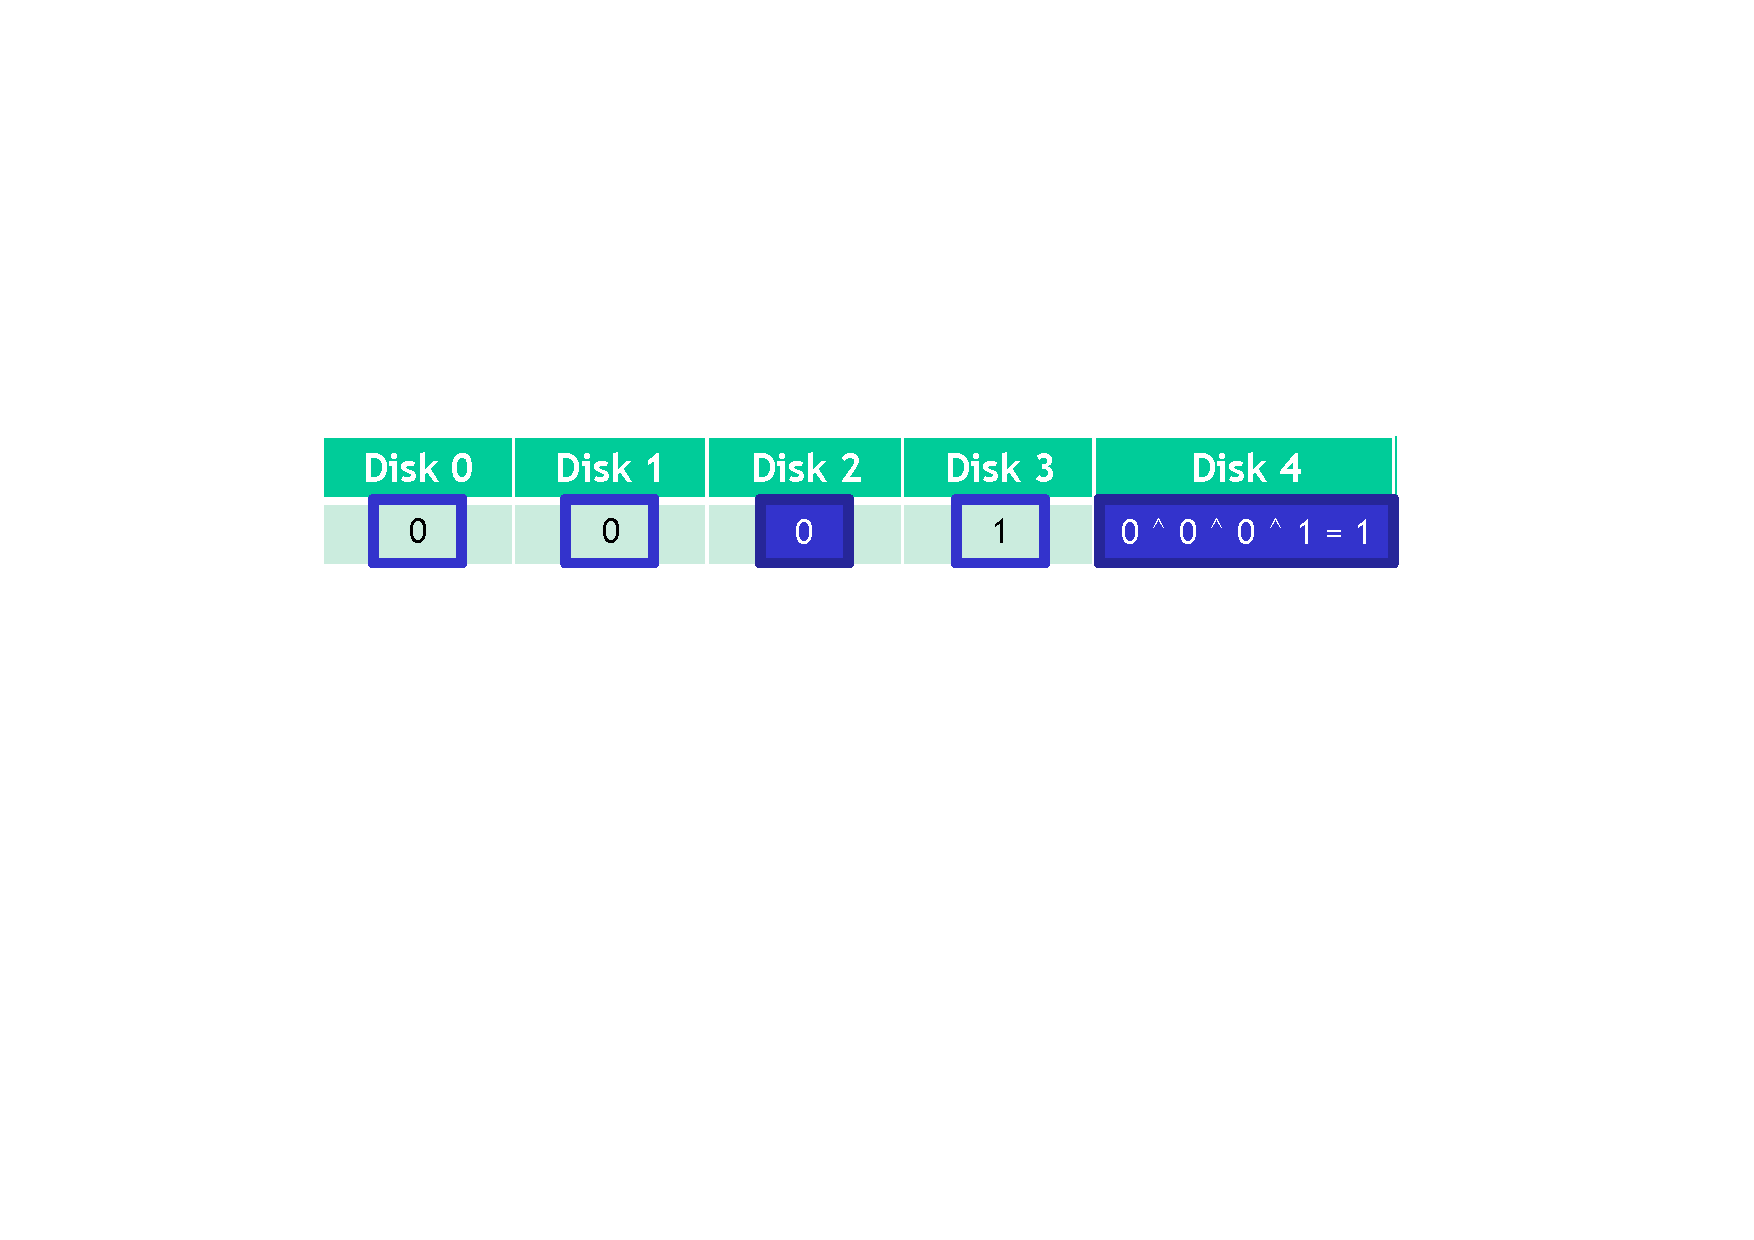
\includegraphics[width=.8\textwidth]{img/raid-7.pdf}
    \end{figure}

    \item \definition{Subtractive parity} (as known as read-modify-writes):\index{read-modify-writes}
    \begin{enumerate}
        \item Read only the old data block to be updated and the old parity block;
        \item Compute the new parity block using:
        \begin{equation*}
            P_{new} = \left(D_{new} \:\veebar\: D_{old}\right) \:\veebar\: P_{old}
        \end{equation*}
        Where $\veebar$ is the logical \texttt{XOR}.
        \item Write the new data block and new parity block to disks.
    \end{enumerate}
    \begin{figure}[!htp]
        \centering
        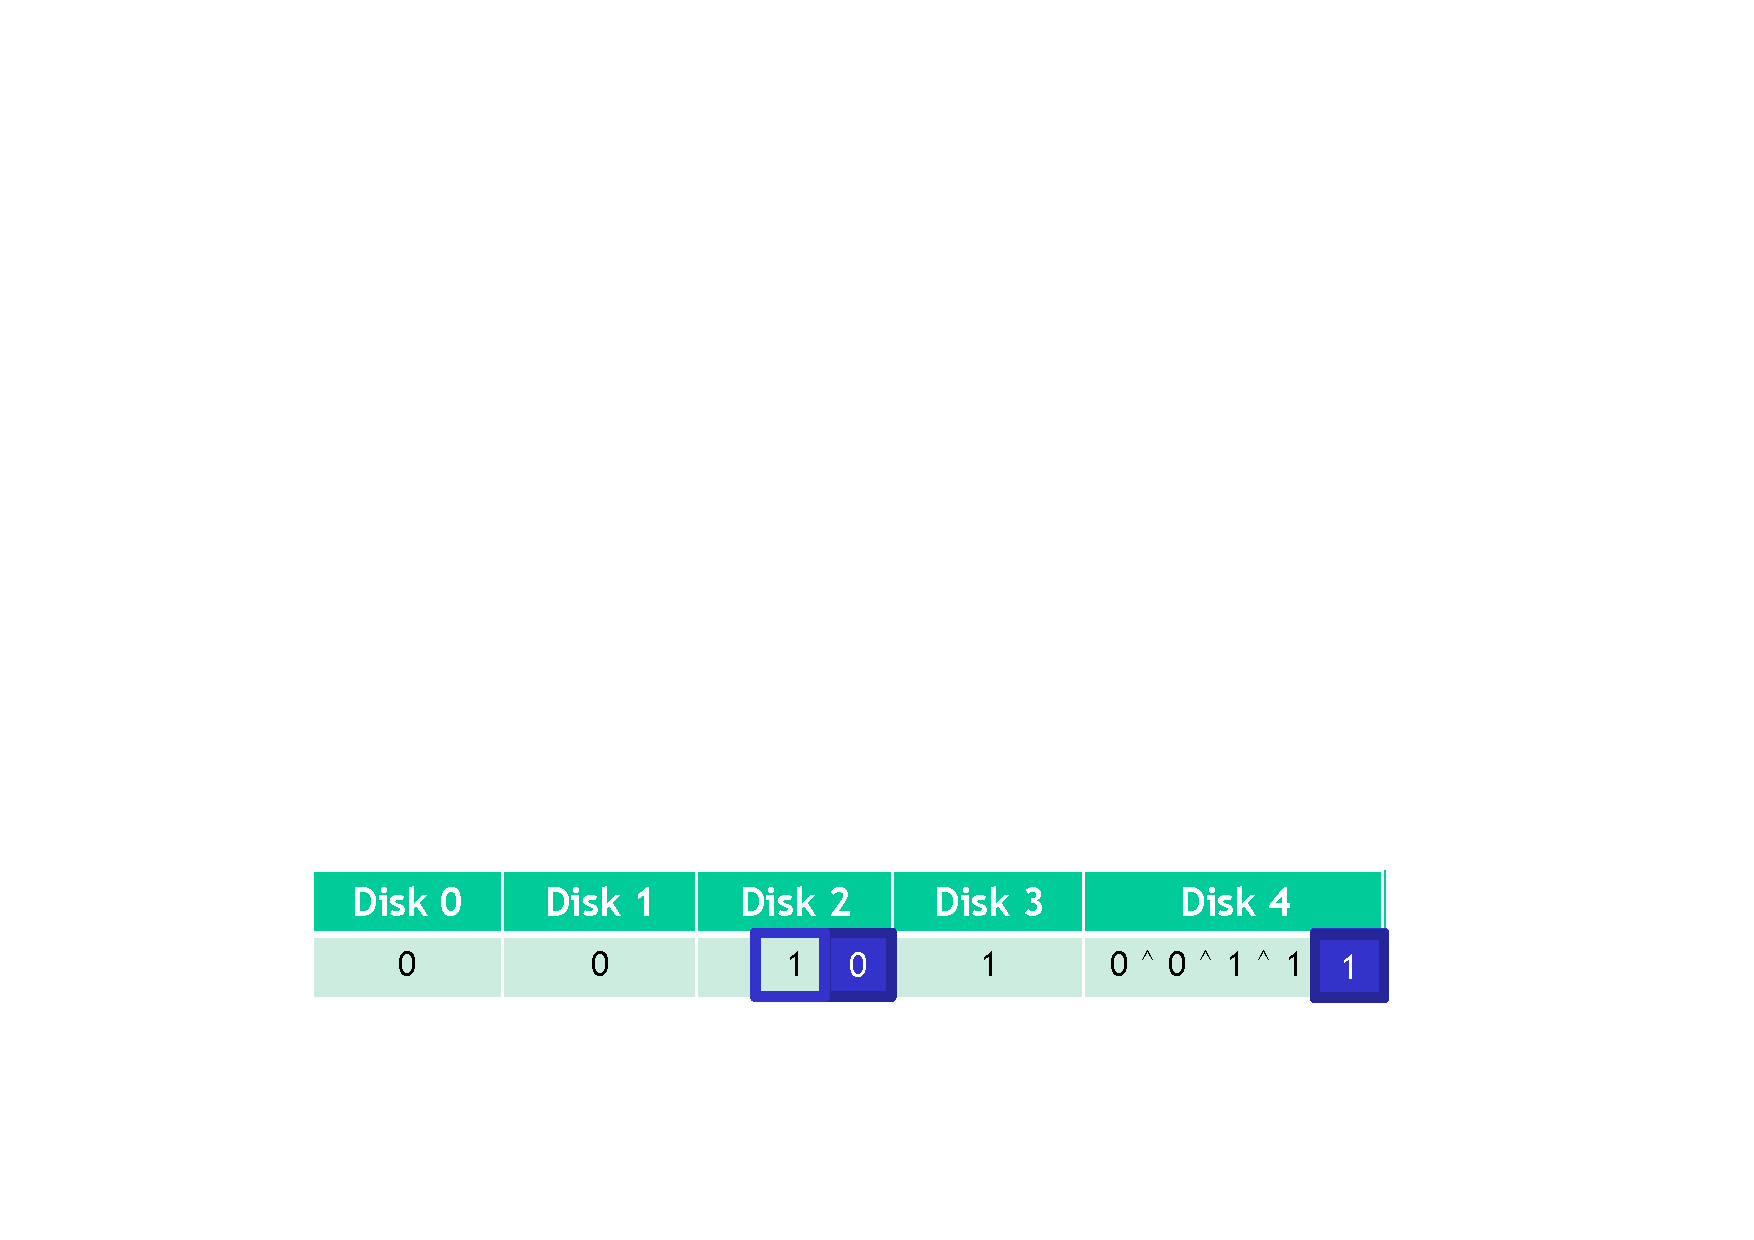
\includegraphics[width=.8\textwidth]{img/raid-8.pdf}
    \end{figure}
\end{itemize}
Despite the \textbf{\underline{sequential write}} does \textbf{not suffer any performance effect} from the parity disk. Because it uses full-stripe write:
\begin{enumerate}
    \item Buffer all data blocks of a stripe
    \item Compute the parity block
    \item Write all data and parity blocks in parallel\cite{raid-and-data-integrity-slides}
\end{enumerate}

\highspace
\begin{flushleft}
    \textcolor{Green3}{\faIcon{chart-bar} \textbf{Analysis}}
\end{flushleft}
\begin{itemize}
    \item \textbf{Capacity}: $N - 1$, where $N$ is the number of disks, and the $-1$ is because one is dedicated to the parity disk.

    \item \textbf{Reliability}: $1$ drive can fail. Massive performance degradation during partial outage.

    \item \textbf{Sequential read/write}: $\left(N - 1\right) \times S$; parallelization across all non-parity blocks in the stripe (parity disk has no effect).

    \item \textbf{Random read}: $\left(N - 1\right) \times R$; reads parallelize over all but the parity drive (parity disk has no effect).

    \item \textbf{Random write}: $R \div 2$; writes serialize due to the parity drive, and each write requires one read and one write of the parity drive.
\end{itemize}
Where $N$ is the number of disks, $S$ is the sequential transfer rate, and $R$ is the random transfer rate.

\newpage

\begin{center}\label{RAID 5}
    \large
    \hypertarget{RAID 5}{\textcolor{Red2}{\textbf{RAID 5}}}
\end{center}

\noindent
RAID 5 \textbf{rotates parity blocks across stripes}.

\highspace
\begin{flushleft}
    \textcolor{Green3}{\faIcon{question-circle} \textbf{When is it used?}}
\end{flushleft}
Unlike in RAID 4, parity information is distributed among the drives. This technique is \textbf{used to improve significantly the random write throughput} against the RAID 4 system.

\highspace
\begin{flushleft}
    \textcolor{Green3}{\faIcon{check} \textbf{Advantages}}
\end{flushleft}
\begin{itemize}
    \item Improved random write despite the RAID 4 system.
\end{itemize}

\highspace
\begin{flushleft}
    \textcolor{Green3}{\faIcon{tools} \textbf{How does it work?}}
\end{flushleft}
The writes are spread roughly evenly across all drives.

\begin{figure}[!htp]
    \centering
    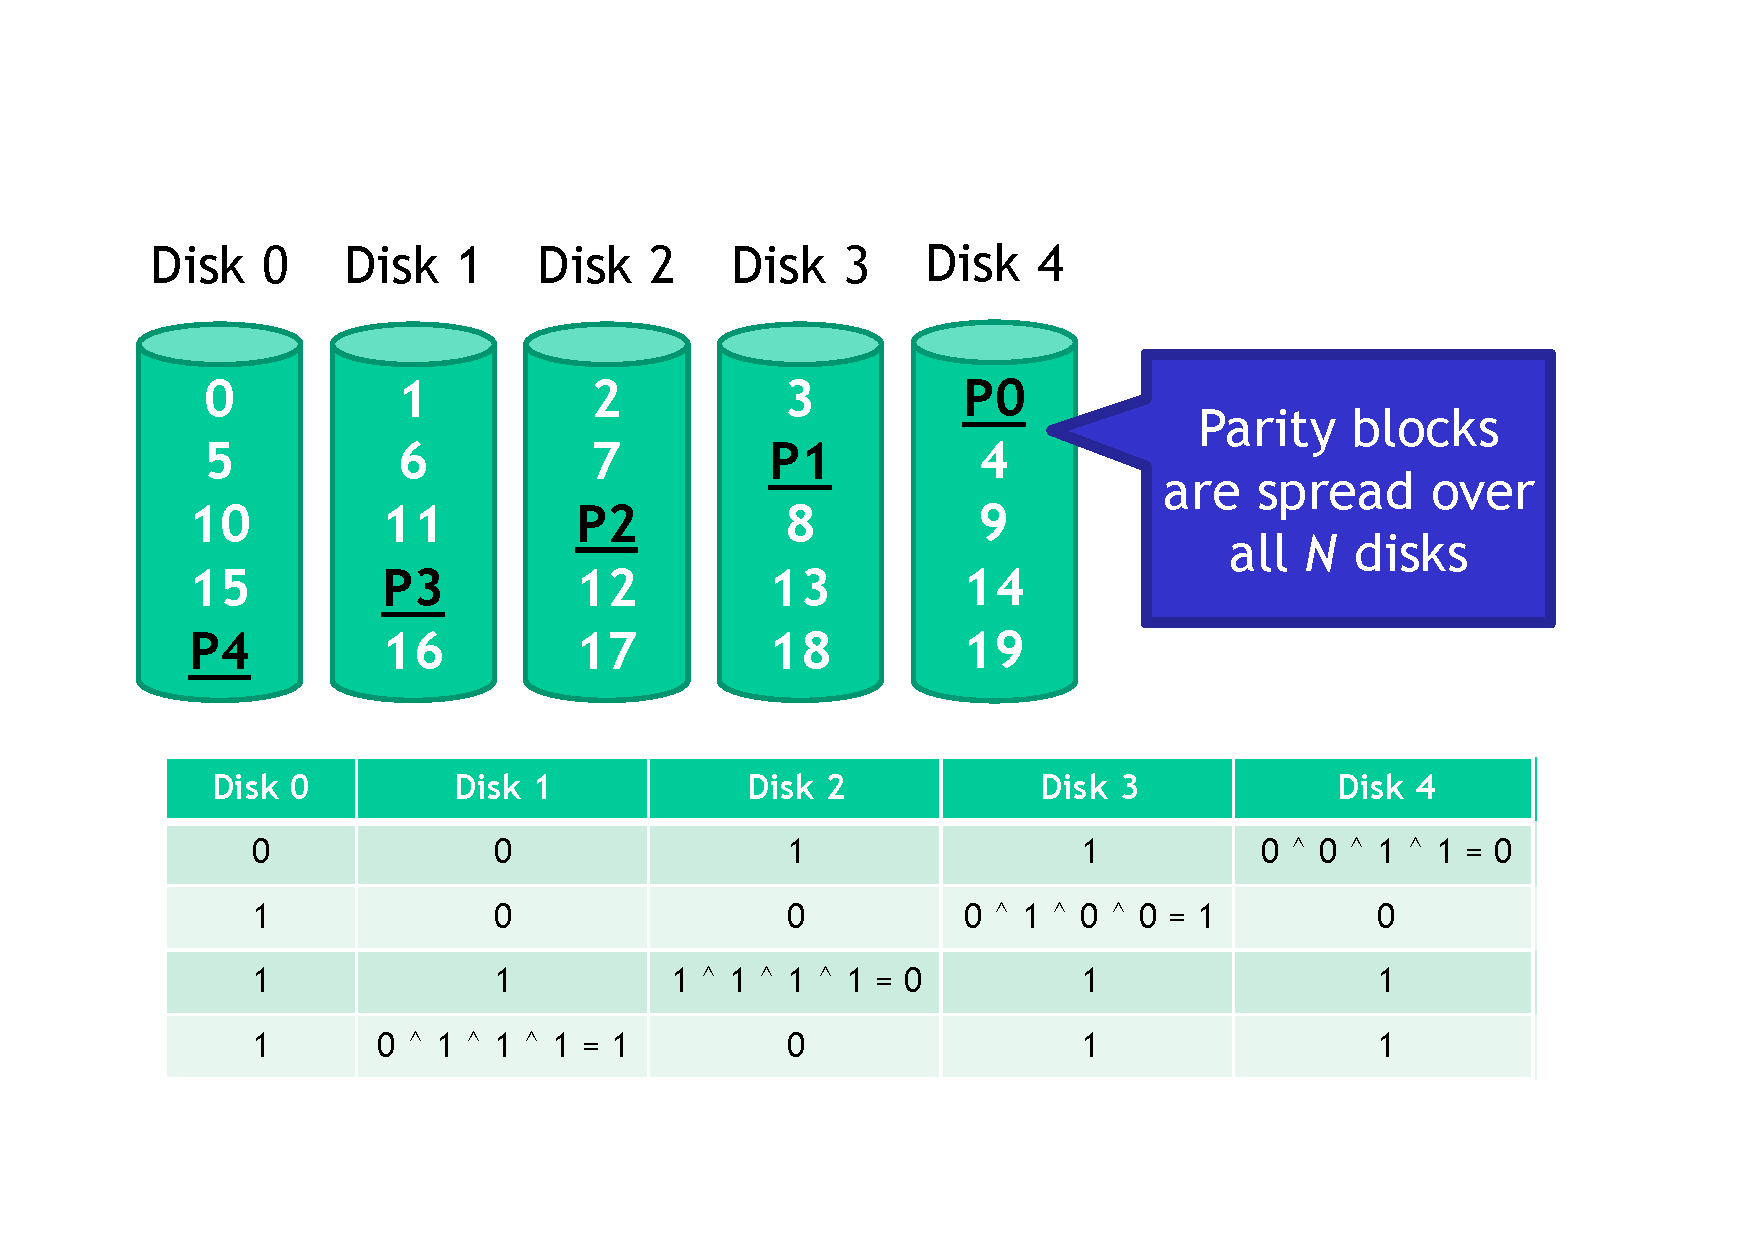
\includegraphics[width=.8\textwidth]{img/raid-9.pdf}
\end{figure}

\noindent
The \textbf{\underline{random write}} in RAID 5 is:
\begin{enumerate}
    \item Read the target block and the parity block
    \item Use subtraction to calculate the new parity block
    \item Write the target block and the parity block
\end{enumerate}
Thus, \textbf{four total operations} (two reads, two writes) \textbf{are distributed across all drives}.

\highspace
\begin{flushleft}
    \textcolor{Green3}{\faIcon{chart-bar} \textbf{Analysis}}
\end{flushleft}
\begin{itemize}
    \item \textbf{Capacity}: $N - 1$ (\textbf{same as RAID 4}), where $N$ is the number of disks.
    \item \textbf{Reliability}: $1$ drive can fail (\textbf{same as RAID 4}). Massive performance degradation during partial outage.
    \item \textbf{Sequential read/write}: (N - 1) * S (\textbf{same as RAID 4}); parallelization across all non-parity blocks in the stripe (parity disk has no effect).
    \item \textbf{Random read}: $N \times R$; unlike RAID 4, \textbf{reads parallelize over all drives}.
    \item \textbf{Random write}: $\left(N \div 4\right) \times R$; unlike RAID 4, \textbf{writes parallelize over all drives}, and each write requires two reads and two writes, hence $N \div 4$.
\end{itemize}
Where $N$ is the number of disks, $S$ is the sequential transfer rate, and $R$ is the random transfer rate.

\longline

\begin{center}\label{RAID 6}
    \large
    \hypertarget{RAID 6}{\textcolor{Red2}{\textbf{RAID 6}}}
\end{center}
RAID 6 can tolerate multiple disk faults (\textbf{more fault tolerance}) concerning RAID 5. It tolerates two concurrent failures.

\highspace
\begin{flushleft}
    \textcolor{Green3}{\faIcon{tools} \textbf{How does it work?}}
\end{flushleft}
It uses Solomon-Reeds codes with two redundancy schemes and requires $N + 2$ disks (where $N$ is the number of disks). Note that the \textbf{minimum set is 4 data disks}.

Unfortunately, it has a \textbf{high overhead for writes} (computation of parities) because each write requires six disk accesses due to the need to update both the P and Q parity blocks (slow writes).

\begin{figure}[!htp]
    \centering
    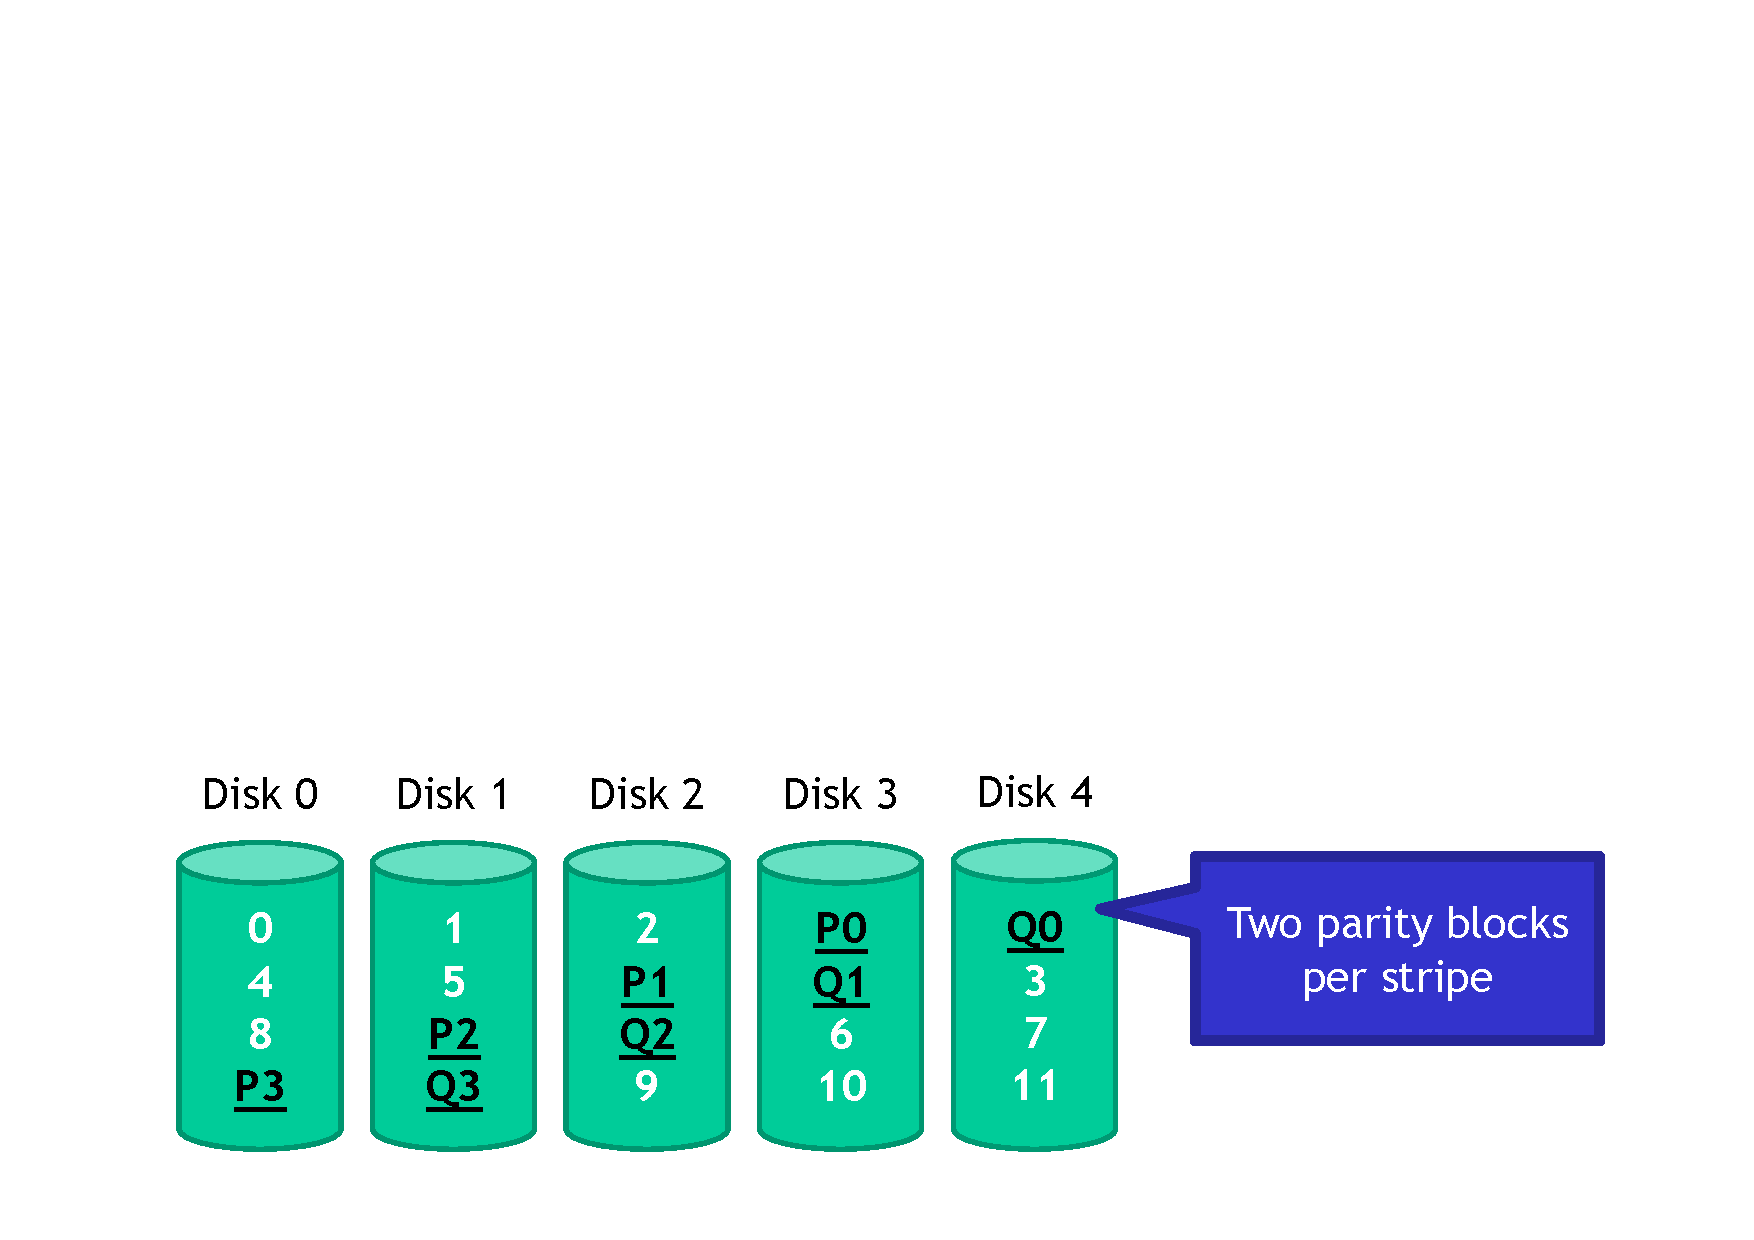
\includegraphics[width=\textwidth]{img/raid-010.pdf}
\end{figure}

\newpage

\begin{center}\label{Comparison and characteristics of RAID levels}
    \large
    \hypertarget{Comparison and characteristics of RAID levels}{\textcolor{Red2}{\textbf{Comparison and characteristics of RAID levels}}}
\end{center}

\noindent
The following table shows eight fundamental properties of the RAID levels.
\begin{itemize}
    \item $N$: number of drives
    \item $R$: random access speed
    \item $S$: sequential access speed
    \item $D$: latency to access a single disk
\end{itemize}
\begin{table}[!htp]
    \centering
    \begin{tabular}{@{} l l l l l @{}}
        \toprule
        & \texttt{RAID 0} & \texttt{RAID 1} & \texttt{RAID 4} & \texttt{RAID 5} \\
        \midrule
        Capacity & $N$ & $N \div 2$ & $N - 1$ & $N - 1$ \\
        Reliability & $0$ & $1 \: \lor : N \div 2$ & $1$ & $1$ \\
        \cmidrule{1-5}
        Sequential Read & $N \times S$ & $\left(N \div 2\right) \times S$ & $\left(N - 1\right) \times S$ & $\left(N - 1\right) \times S$ \\
        Sequential Write & $N \times S$ & $\left(N \div 2\right) \times S$ & $\left(N - 1\right) \times S$ & $\left(N - 1\right) \times S$ \\
        Random Read & $N \times R$ & $N \times R$ & $\left(N - 1\right) \times R$ & $N \times R$ \\
        Random Write & $N \times R$ & $\left(N \div 2\right) \times R$ & $R \div 2$ & $\left(N \div 4\right) \times R$ \\
        \cmidrule{1-5}
        Read & $D$ & $D$ & $D$ & $D$ \\
        Write & $D$ & $D$ & $2 \times D$ & $2 \times D$ \\
        \bottomrule
    \end{tabular}
    \caption{Comparison of RAID levels.}
\end{table}

\noindent
Where the throughput is:
\begin{itemize}
    \item Sequential Read
    \item Sequential Write
    \item Random Read
    \item Random Write
\end{itemize}
And the latency is:
\begin{itemize}
    \item Read
    \item Write
\end{itemize}

\newpage

\begin{figure}[!htp]
    \centering
    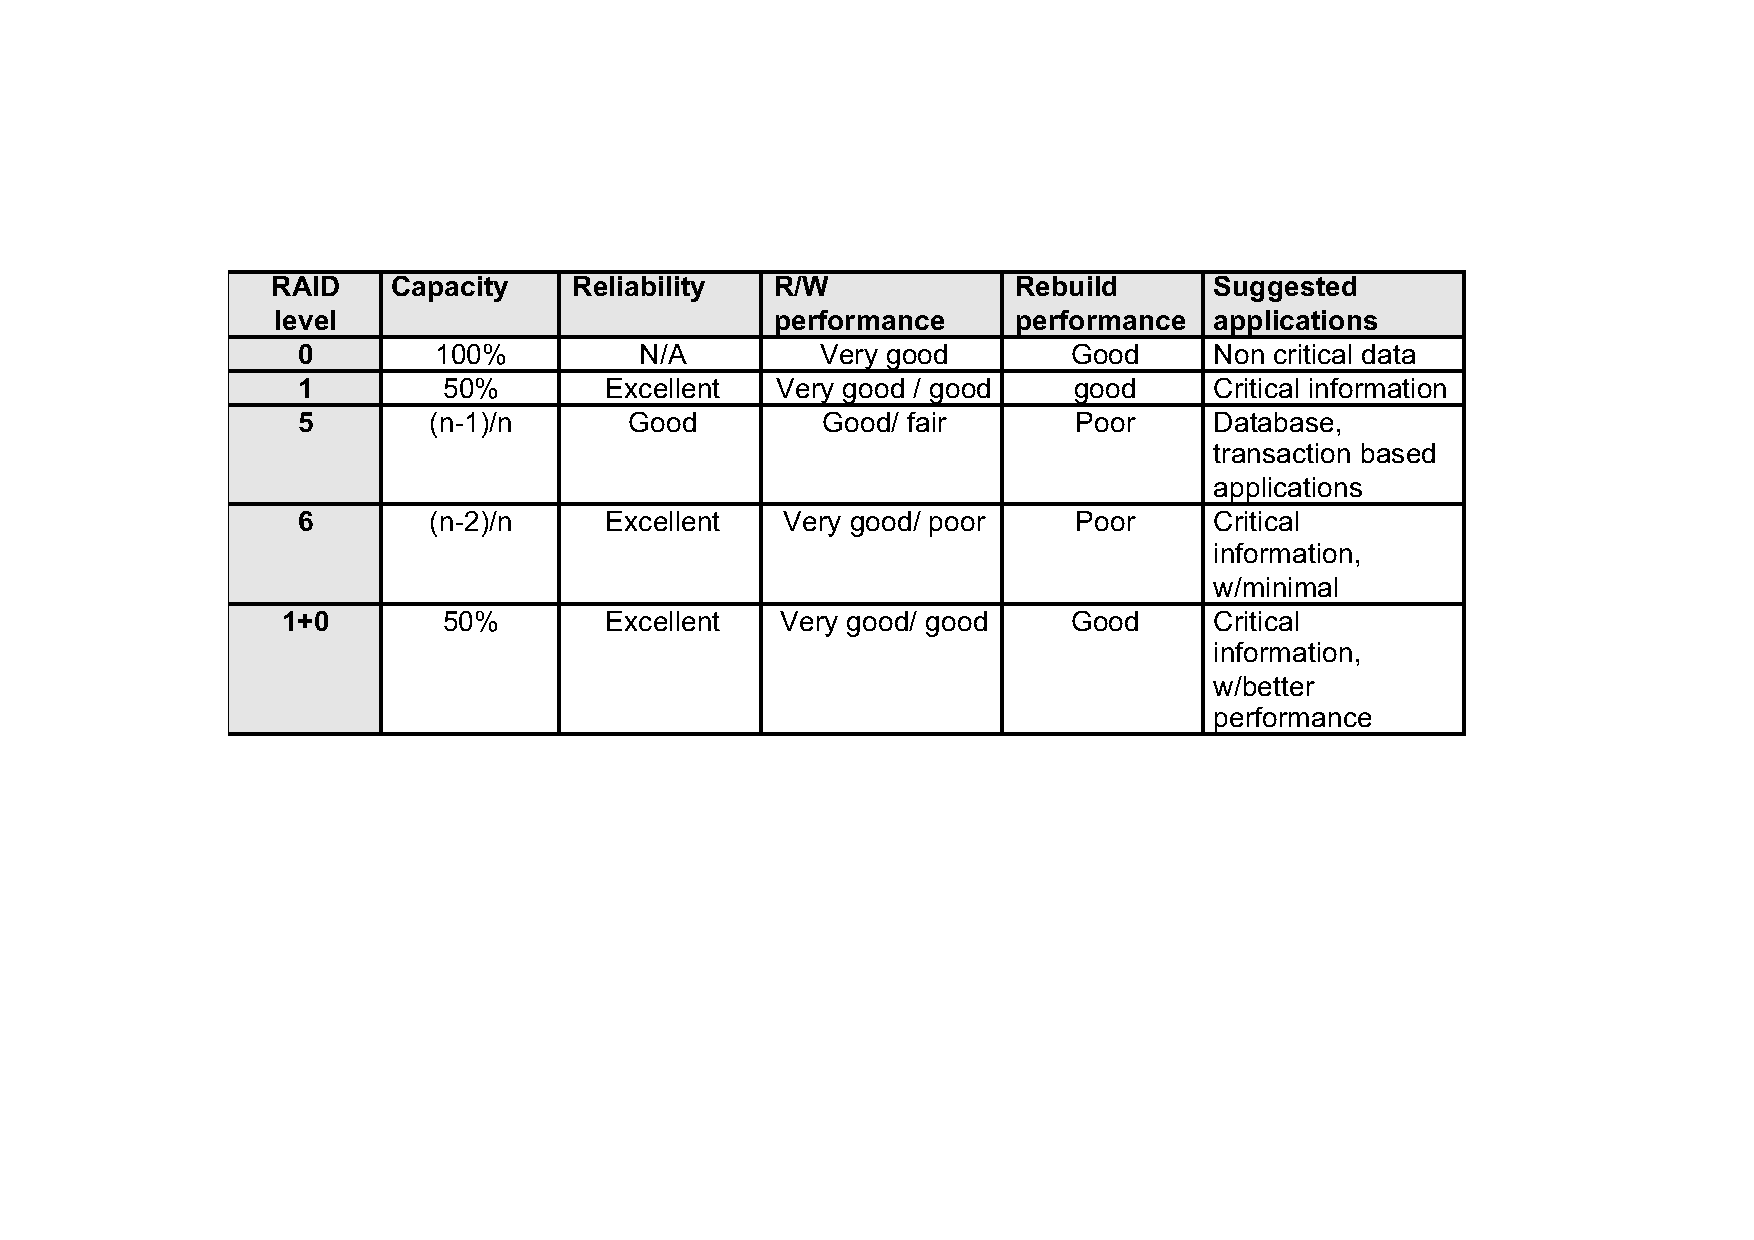
\includegraphics[width=\textwidth]{img/raid-011.pdf}
    \caption{Characteristics of RAID levels.}
\end{figure}

\noindent
\textbf{RAID 0} has the \underline{best performance} and \underline{most capacity}.

\highspace
\textbf{RAID 1} (10 better than 01) or \textbf{RAID 6} have the \underline{greatest error recovery}.

\highspace
\textbf{RAID 5} has the better \textbf{\emph{balance}} between \underline{space}, \underline{performance}, and \underline{recoverability}.

\newpage

\paragraph{DAS, NAS and SAN}

As the last argument, we introduce \textbf{three different typologies} of storage systems:
\begin{itemize}
	\item \definition{Direct Attached Storage (DAS)} is a \textbf{storage system directly attached to a server or workstation}. They are visible as disks/volumes by the client OS.
	
	\item \definition{Network Attached Storage (NAS)} is a \textbf{computer connected to a network that provides only file-based data storage services} (e.g. FTP, Network File System) to other devices on the network and is visible as File Server to the client OS.
	
	\item \definition{Storage Area Networks (SAN)} are \textbf{remote storage units connected to a PC using a specific networking technology} (e.g. Fiber Channel) and are visible as disks/volumes by the client OS.
\end{itemize}
In the following schema, we can see a simple architectural comparison.
\begin{figure}[!htp]
	\centering
	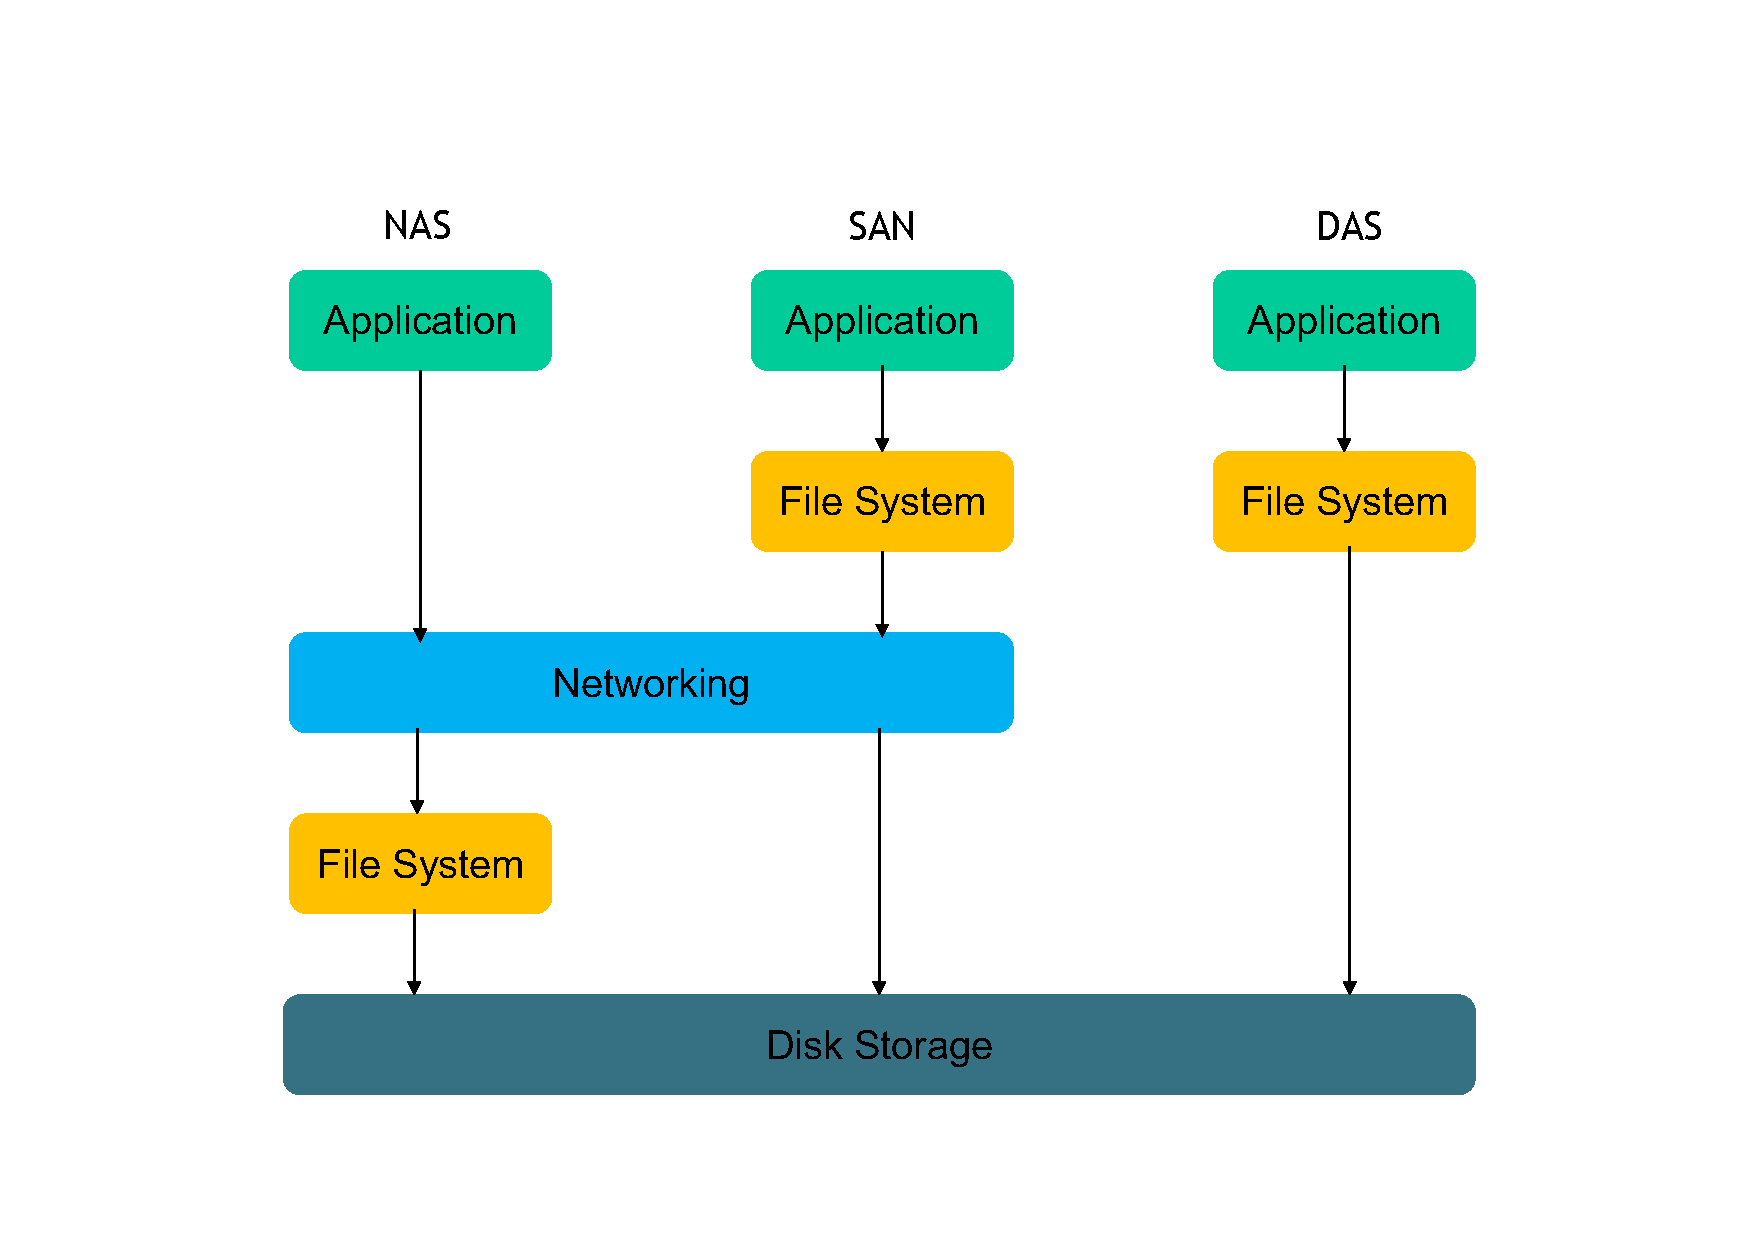
\includegraphics[width=.8\textwidth]{img/nas-san-das-1.pdf}
\end{figure}

\begin{flushleft}
	\textcolor{Red2}{\faIcon{check} \textbf{DAS features}}
\end{flushleft}
DAS is a \textbf{storage system directly attached to a server or workstation}. The term is used to differentiate non-networked storage from SAN and NAS. The \textbf{main features} are:
\begin{itemize}
	\item Limited scalability.
	\item Complex manageability.
	\item Limited performance.
	\item To read files in other machines (the "file sharing" protocol of the OS must be used).
\end{itemize}
Note that all the \textbf{external disks connected to a PC with a point-to-point protocol can be considered DAS}.
\begin{figure}[!htp]
	\centering
	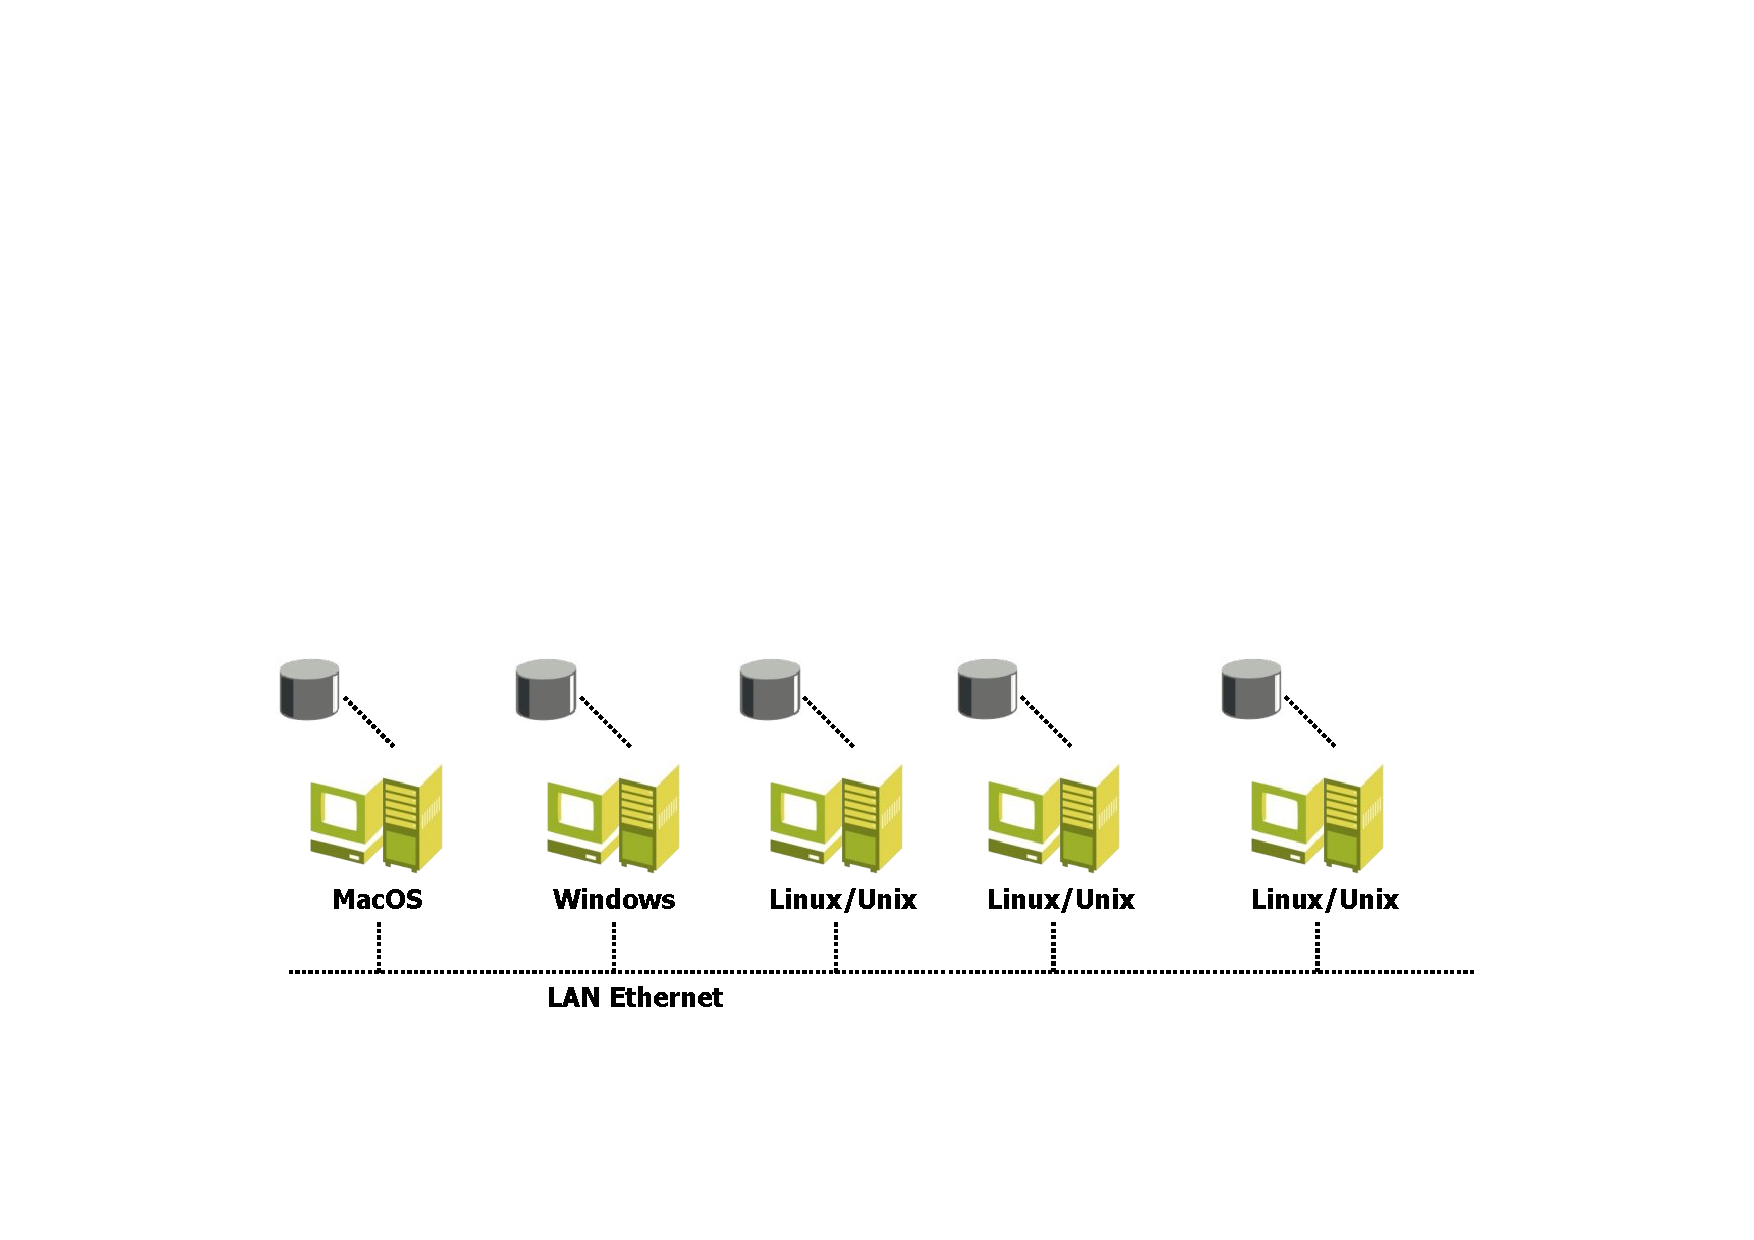
\includegraphics[width=\textwidth]{img/nas-san-das-2.pdf}
	\caption{DAS architecture.}
\end{figure}

\highspace
\begin{flushleft}
	\textcolor{Red2}{\faIcon{check} \textbf{NAS features}}
\end{flushleft}
A NAS unit is a \textbf{computer connected to a network that provides only file-based data storage services to other devices on the network}. NAS systems contain one or more hard disks, often organized into logical redundant storage containers or RAID. Finally, \textbf{NAS provides file-access services to the hosts connected to a TCP/IP network through Networked File Systems/SAMBA}. Each NAS element has its IP address. Furthermore, each NAS has good scalability.

\highspace
The \textbf{main differences between DAS and NAS} are:
\begin{itemize}
	\item DAS is simply an \textbf{extension of an existing server} and is \textbf{not necessarily networked}.
	\item NAS is designed as an easy and self-contained solution for \textbf{sharing files over the network}.
\end{itemize}
Regarding \textbf{performance}, NAS depends mainly on the speed and congestion of the network.
\begin{figure}[!htp]
	\centering
	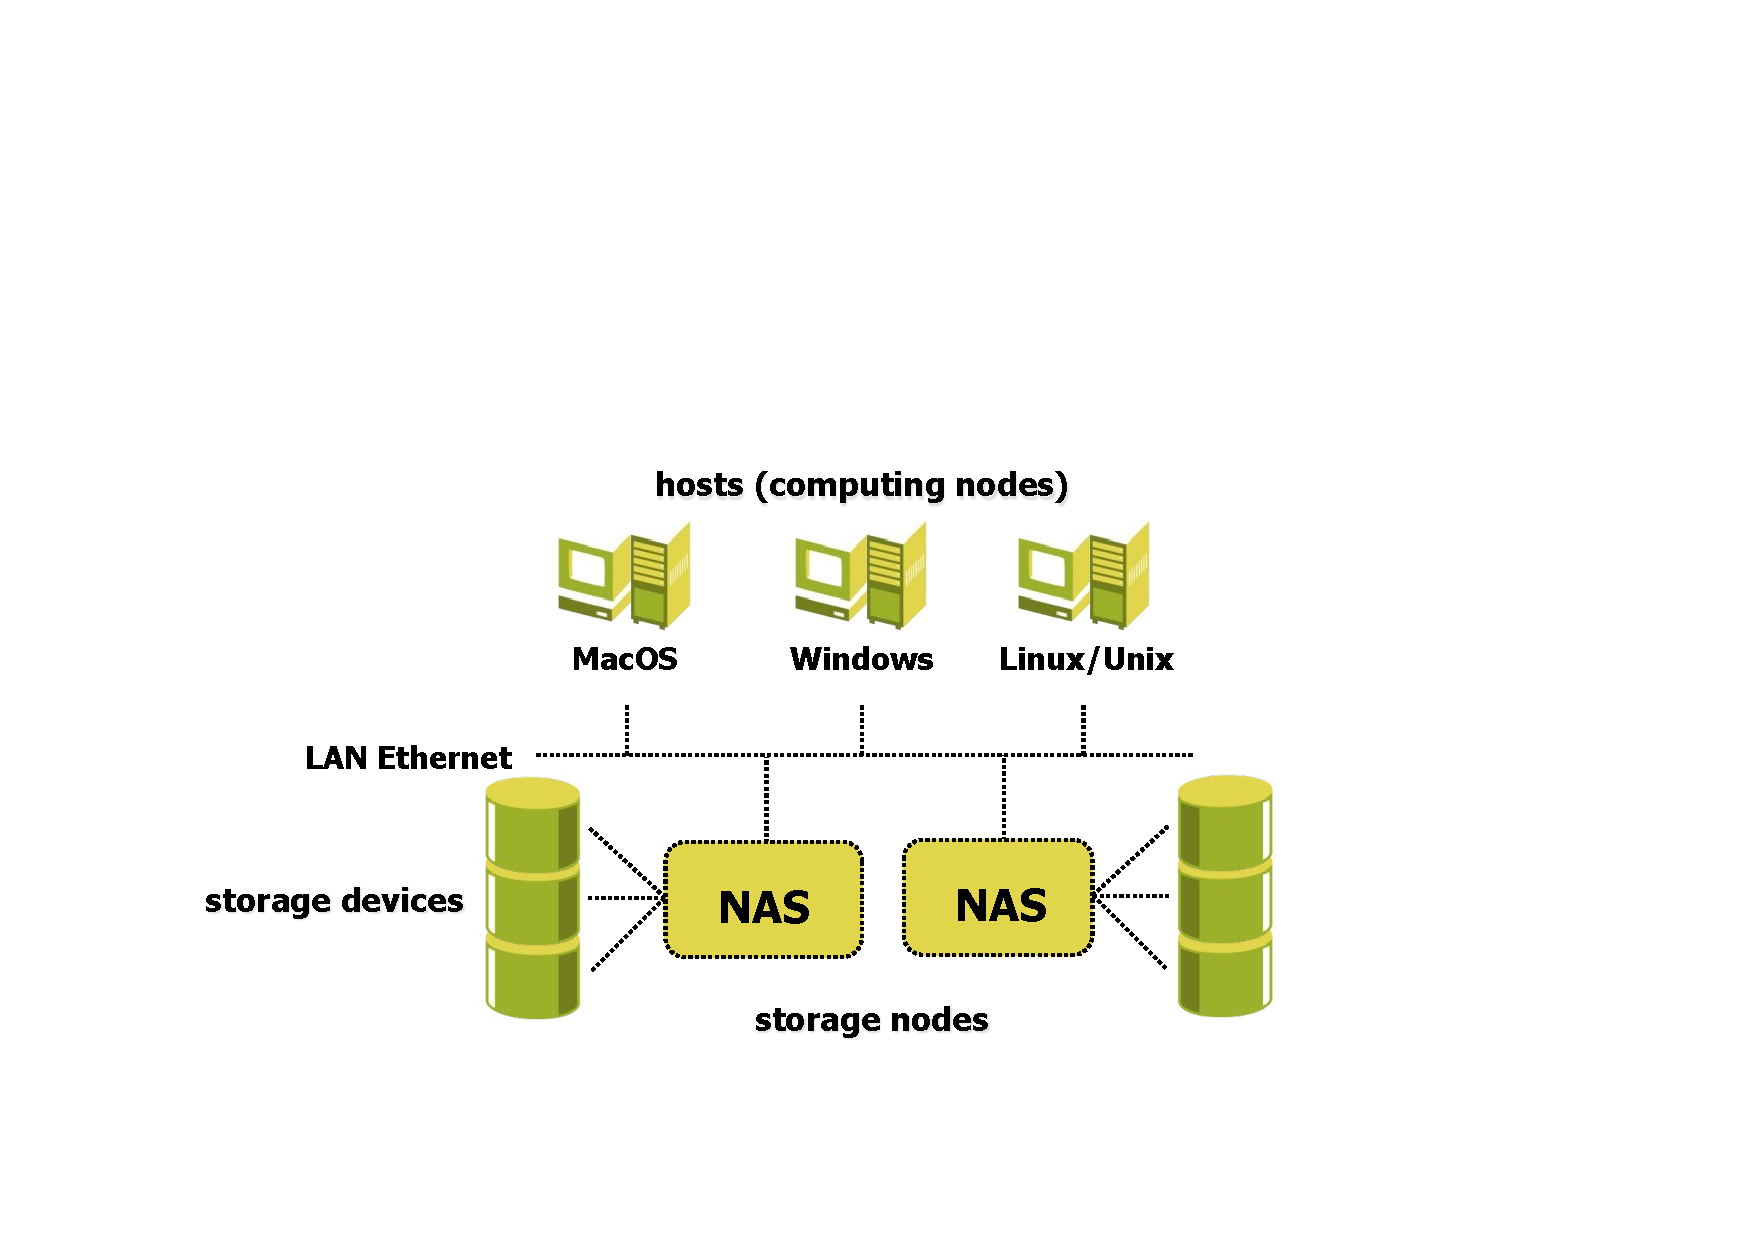
\includegraphics[width=.7\textwidth]{img/nas-san-das-3.pdf}
	\caption{NAS architecture.}
\end{figure}

\highspace
\begin{flushleft}
	\textcolor{Red2}{\faIcon{check} \textbf{SAN features}}
\end{flushleft}
SANs are remote \textbf{storage units connected to servers using a specific networking technology}. SANs have a particular network dedicated to accessing storage devices. It has two distinct networks: one TCP/IP and another dedicated network (e.g. Fiber Channel). It has a high scalability.

\highspace
The \textbf{main difference between a NAS and a SAN} is that:
\begin{itemize}
	\item \textbf{NAS appears to the client OS as a file server}. Then, the client can map network drives to shares on that server.
	
	\item \textbf{A disk available through a SAN still appears to the client OS as a disk}. It will be visible in the disks and volumes management utilities (along with the client's disks) and available to be formatted with a file system.
\end{itemize}
\begin{figure}[!htp]
	\centering
	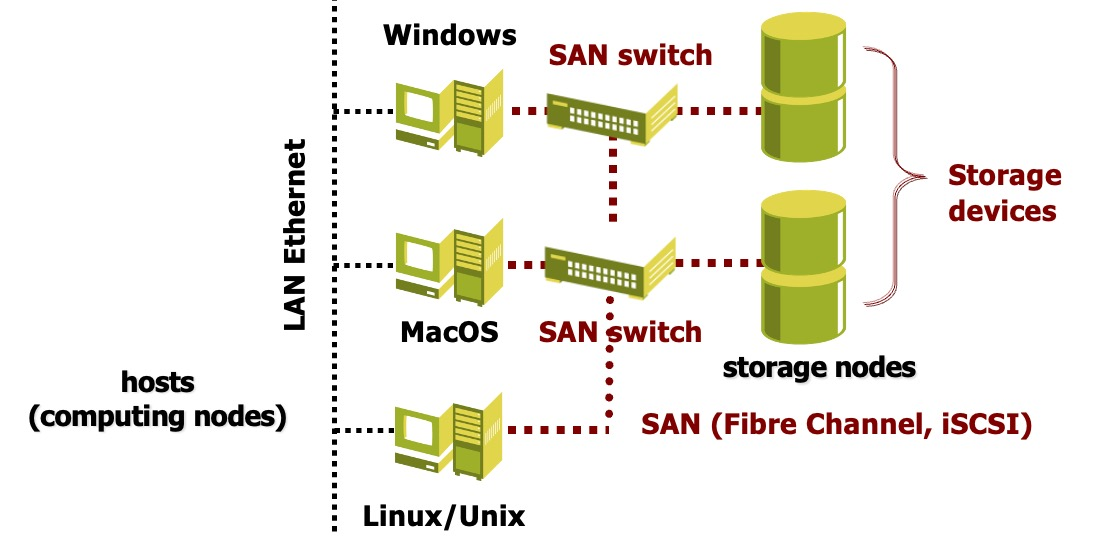
\includegraphics[width=.8\textwidth]{img/nas-san-das-4.png}
	\caption{SAN architecture.}
\end{figure}

\begin{figure}[!htp]
	\centering
	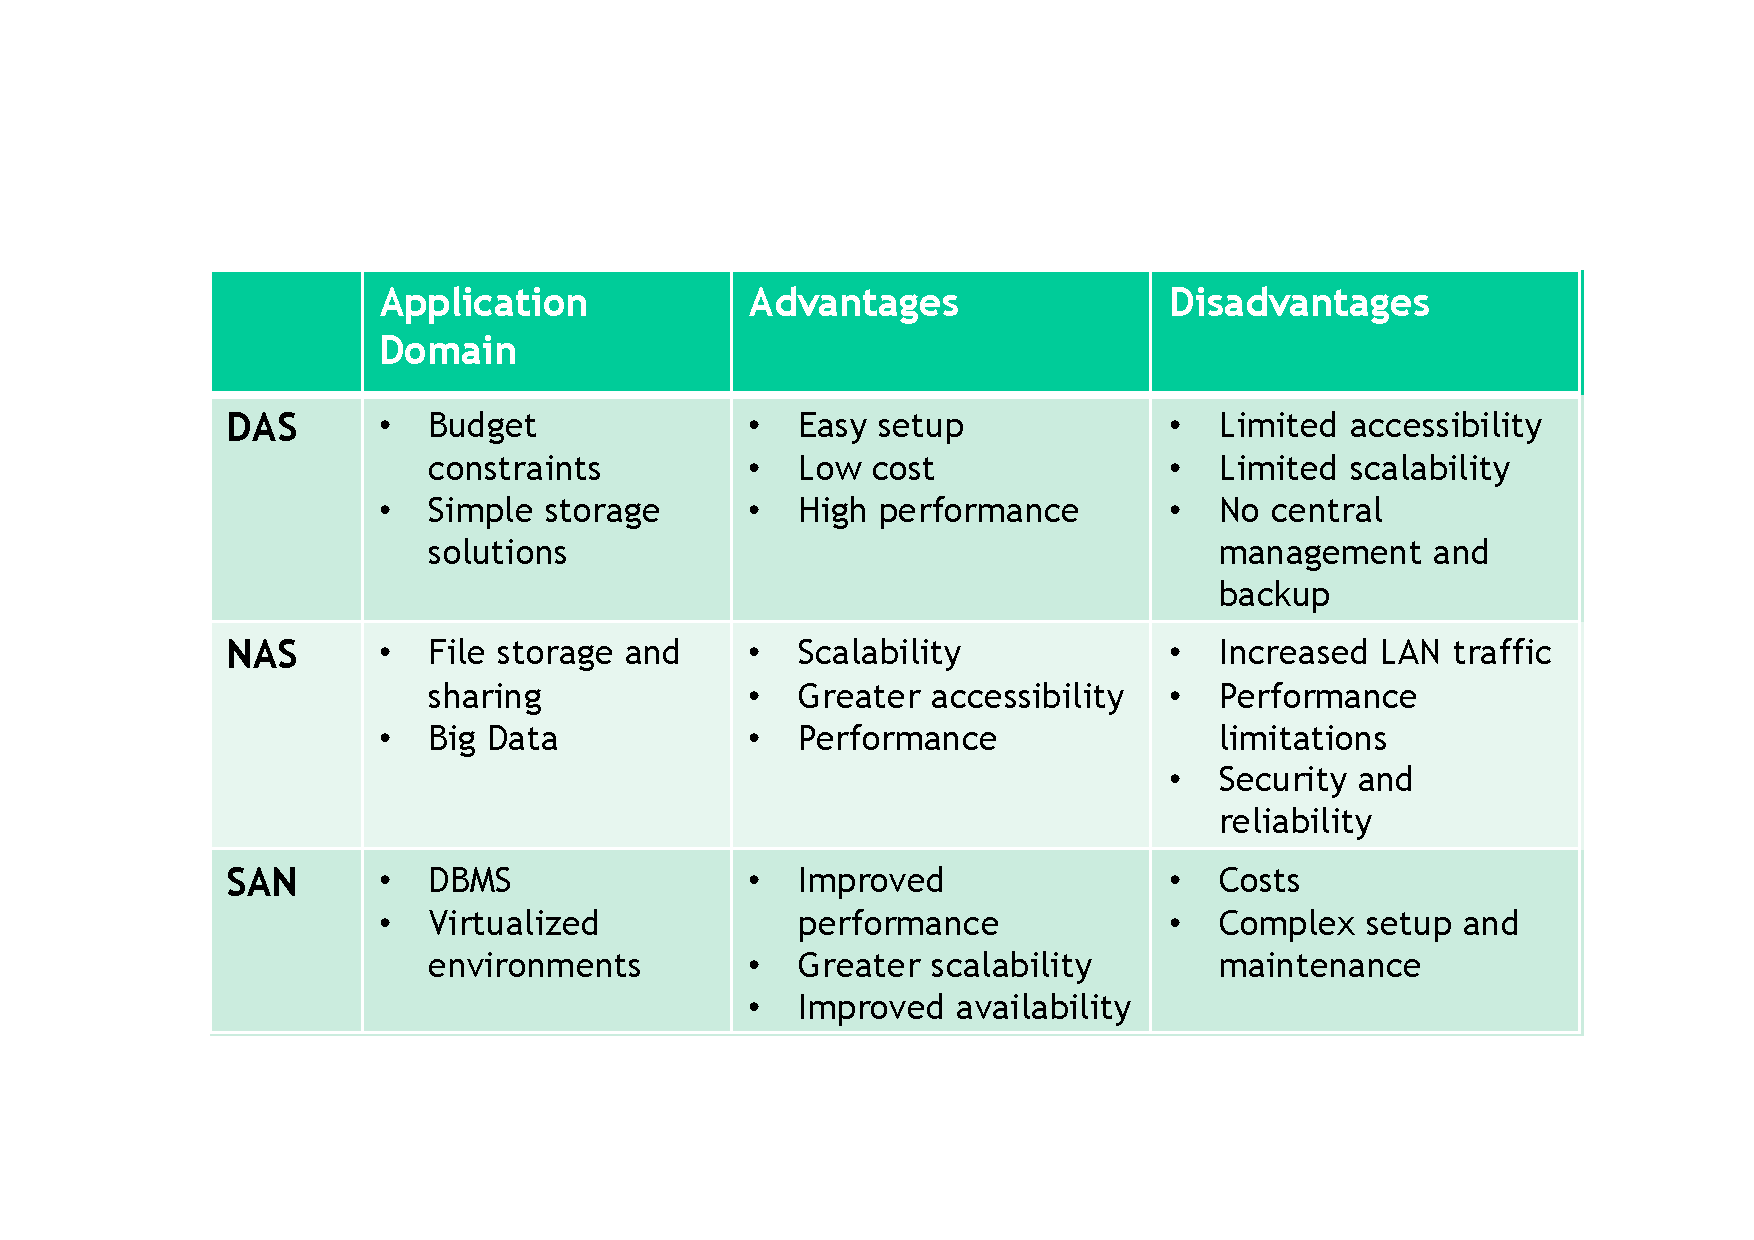
\includegraphics[width=\textwidth]{img/nas-san-das-5.pdf}
	\caption{DAS vs. NAS vs. SAN}
\end{figure}

\newpage

\subsubsection{Networking (architecture and technology)}\label{subsubsection: Networking (architecture and technology)}
